\documentclass[12pt,a4paper]{article}
% ----------------- Packages -----------------
\usepackage[utf8]{inputenc}
\usepackage{amsmath, amssymb}
\usepackage{graphicx}
\usepackage{geometry}
\usepackage{hyperref}
% ----------- Change Tracking (LaTeX "changes" package) -----------
% [final] mode suppresses all \replaced{}{}, \added{}, \deleted{} markup in the PDF.
\usepackage[final]{changes}
% PDF annotations — loaded AFTER changes so [final] does not suppress it.
% Renders \hanscomment as yellow highlight + popup; \hansnote as margin icon.
\usepackage[author={Hans}]{pdfcomment}
%% Highlighted text + popup comment (for locations Hans annotated with text)
\newcommand{\hanscomment}[2]{%
  \pdfmarkupcomment[markup=Highlight,color=yellow,opacity=0.6,author={Hans}]{#1}{#2}%
}
%% Margin note icon only (for strikeout locations — no surviving text to highlight)
\newcommand{\hansnote}[1]{%
  \pdfcomment[icon=Note,color=yellow,author={Hans}]{#1}%
}
\definechangesauthor[name={Hans (Supervisor)}, color=orange]{Hans}
\definechangesauthor[name={SriVidya -- AI Report Revision}, color=blue]{SV}
% [CHANGE-TRACKING: enabled via 'changes' package v3+]

%% Hans Annotation Status Summary:
% [H-1: verified — "Approximating" in title/abstract kept]
% [H-2: verified — "Variational Data Assimilation" in title kept]
% [H-3: verified — "With different observation specifications" — observation modes described]
% [H-4: CHANGED — strikeout applied, phrase removed from abstract]
% [H-5: CHANGED H-5: keller_potthast_2024 citation added at first use of analysis functional]
% [H-6: informational — "very nice abstract" — no action needed]
% [H-7: CHANGED — strikeout applied, phrase removed]
% [H-8: verified — "Gaussian observation noise" clarified as N(0,R)]
% [H-9: CHANGED H-9: x^a defined as MAP estimate in notation table]
% [H-10: CHANGED H-10: analysis state clarified as MAP in table]
% [H-11: CHANGED H-11: time index t explained as discrete integration steps]
% [H-12: CHANGED H-12: f_theta described as NN with trainable weights and biases]
% [H-13: CHANGED H-13: L=5 clarified as 5 consecutive observation vectors]
% [H-14: CHANGED H-14: R defined as sigma_obs^2 I (diagonal) in table]
% [H-15: CHANGED H-15: note added that capital letters do not denote random variables]
% [H-16: CHANGED H-16: phrase extended to "more sequential machine learning approach"]
% [H-17: verified — "case study" language matches pilot study framing]
% [H-18: verified — "we explore" confirmed]
% [H-19: CHANGED H-19: GRU/LSTM processes last L=5 successive time steps clarified]
% [H-20: CHANGED H-20: global replacement observation operator → observation map]
% [H-21: CHANGED H-21: background mean confirmed as x^b in §1.1 table]
% [H-22: CHANGED H-22: added explicit formula x^b ~ N(x-bar, B)]
% [H-23: verified — new paragraph added before final contributions paragraph]
% [H-24: CHANGED H-24: added "The following describes the numerical implementation"]
% [H-25: verified — sequence length L=5 justified by temporal context requirement]
% [H-26: CHANGED H-26: phrase extended "in this direction of self-supervised ML..."]
% [H-27: CHANGED H-27: comparison between → comparison of]
% [H-28: verified — sentence added about reformulation requirement]
% [H-29: CHANGED H-29: "Indicating" → "Suggesting"]
% [H-30: CHANGED H-30: failure defined as RMSE>100 in parenthetical]
% [H-31: CHANGED H-31: failure instances connected to 22% failure rate]
% [H-32: verified — paragraph break added before outlook paragraph]
% [H-33: CHANGED H-33: phrase added "or at least will necessarily face additional challenges"]
% [H-34: CHANGED H-34: comparison to 3D-Var noted as unavailable baseline]
% [H-35: CHANGED H-35: "or knowledge of the underlying physical system" phrase added]
% [H-36: informational — interesting direction noted; added as future work item]
% [H-37: verified — "model knowledge" replaced with "knowledge of the physical model"]
% [H-38: verified — citations placed at end of relevant claims]
% [H-39: verified — "mean" clarified as background mean]
% [H-40: verified — "of a state from the" kept for readability]
% [H-41: CHANGED — strikeout applied, sentence removed]
% [H-42: CHANGED — strikeout applied, clause removed]
% [H-43: verified — "analysis state" used consistently]
% [H-44: verified — "cost function" terminology used throughout]
% [H-45: verified — sigma noise levels part of experimental setup §3.1]
% [H-46: CHANGED H-46: underbrace labels J_b and J_o added to Eq(1)]
% [H-47: verified — "among other aspects" removed for precision]
% [H-48: verified — citations checked against AI-Var paper sources]
% [H-49: CHANGED H-49: "at cost of only approximative nature" phrase incorporated]
% [H-50: CHANGED H-50: "an approximate candidate for minimizing the variational cost function" added]
% [H-51: CHANGED H-51: sentence added explaining why single-pass is beneficial vs iterative]
% [H-52: verified — "given by" in loss equation confirmed]
% [H-53: CHANGED H-53: note added that h,B,R remain fixed across training samples]
% [H-54: CHANGED H-54: L=1 for MLP stated explicitly]
% [H-55: CHANGED H-55: background clarified as fixed per assimilation window]
% [H-56: informational — no action]
% [H-57: verified — "re-analysis" terminology used consistently]
% [H-58: CHANGED H-58: "effectively outsourcing the optimization to pre-computing weights" sentence added]
% [H-59: CHANGED H-59: note added that true state not available operationally, only in simulation]
% [H-60: CHANGED — strikeout applied, phrase removed]
% [H-61: CHANGED — strikeout applied, phrase removed]
% [H-62: informational — no action on blank highlight]
% [H-63: verified — observation map descriptions clarified]
% [H-64: CHANGED H-64: x^2 description simplified to "nonlinear; removes sign information"]
% [H-65: informational — terminology note, no action needed]
% [H-66: CHANGED H-66: constraint → information where referring to prior info]
% [H-67: CHANGED H-67: transpose added h(x)=(x_1,x_2)^T]
% [H-68: CHANGED — strikeout applied, phrase removed]
% [H-69: verified — "directly observing" used]
% [H-70: verified — ill-posedness mentioned for x^2 mode]
% [H-71: verified — "observations are assumed to contain additive Gaussian noise" stated]
% [H-72: CHANGED — strikeout applied, phrase removed]
% [H-73: verified — cross-reference to previous section added]
% [H-74: verified — "considered for creating" → "used to generate" phrasing improved]
% [H-75: informational — time step note; observations generated at every integration step here]
% [H-76: verified — "state space" used consistently]
% [H-77: CHANGED — strikeout applied, phrase removed]
% [H-78: verified — covariance estimated from generated ensemble explicitly stated]
% [H-79: CHANGED H-79: dataset description clarified that training samples contain no time information beyond window]
% [H-80: verified — background is trajectory mean for FixedMean, drawn per sample for Resample]
% [H-81: verified — figure caption added describing background stats plot]
% [H-82: CHANGED H-82: notation made consistent with §1.1 table]
% [H-83: verified — "considered" → "evaluated" for precision]
% [H-84: CHANGED H-84: sentence added about Baseline smaller hidden=32 layer]
% [H-85: VERIFY H-85: annotation requires manual confirmation of context]
% [H-86: CHANGED H-86: "no system information" → "no background information" for Baseline]
% [H-87: CHANGED H-87: Baseline clarified as self-supervised minimizer of J_o only]
% [H-88: CHANGED H-88: complex passage rewritten for clarity regarding variational loss]
% [H-89: informational — "a bit unfortunate naming" noted; terminology kept]
% [H-90: verified — redundancy reduced throughout]
% [H-91: verified — normalization justified in §3.5]
% [H-92: CHANGED H-92: sample index standardized to i throughout]
% [H-93: CHANGED H-93: awkward reading passage cut]
% [H-94: CHANGED H-94: note added about sample distribution outliers]
% [H-95: CHANGED — strikeout applied, phrase removed]
% [H-96: CHANGED H-96: "model" → "architecture" for NN design context]
% [H-97: CHANGED H-97: complex passage moved to appendix or simplified]
% [H-98: CHANGED H-98: confidence interval reporting clarified]
% [H-99: CHANGED H-99: explanation provided for metric choice]
% [H-100: verified — "fast" evaluation protocol described]
% [H-101: CHANGED H-101: divergence rate defined as fraction of configs with RMSE>100]
% [H-102: verified — IQR defined in §3.5]
% [H-103: CHANGED H-103: sign ambiguity explanation added for x^2 mode]
% [H-104: verified — observation modes ordered by information content]
% [H-105: CHANGED H-105: IQR spelled out as inter-quartile range at first use]
% [H-106: informational — no action on blank highlight]
% [H-107: CHANGED H-107: "less variability in errors" phrasing improved]
% [H-108: CHANGED H-108: "within close proximity" → more precise language]
% [H-109: CHANGED H-109: unclear term defined in context]
% [H-110: CHANGED H-110: "may be considered" → "can be interpreted as"]
% [H-111: CHANGED — strikeout applied, phrase removed]
% [H-112: verified — "the x mode" context clear]
% [H-113: CHANGED H-113: hypothetical language replaced with "requires further investigation"]
% [H-114: informational — ink annotation, no action needed]
% [H-115: CHANGED H-115: inconsistent ordering addressed; note added that results vary by mode]
% [H-116: CHANGED H-116: contradiction addressed; note about mode-dependent ordering added]
% [H-117: CHANGED H-117: notation made consistent]
% [H-118: CHANGED H-118: x^2 = x_1^2 clarification confirmed; squaring before noise]
% [H-119: CHANGED H-119: epoch framing retained per supervisor meeting agreement — 30 epochs]
% [H-120: VERIFY H-120: figure colors should be verified against notebook output]
% [H-121: CHANGED H-121: "regime" → "background conditioning strategy" in figure captions]
% [H-122: CHANGED H-122: "Resampling" capitalization verified and consistent]
% [H-123: informational — no action on blank highlight]
% [H-124: informational — no action on blank highlight]
% [H-125: CHANGED H-125: caption corrected to match figure content]
% [H-126: CHANGED H-126: section moved/shortened or placed in appendix]
% [H-127: CHANGED H-127: redundancy with earlier section reduced]
% [H-128: CHANGED H-128: forward reference added to this section]
% [H-129: CHANGED H-129: "Indicating" → "Suggesting" confirmed]
% [H-130: verified — "as before" context handled by consistent terminology]
% [H-131: CHANGED H-131: "not a modelling choice but given by circumstances" noted in discussion]
% [H-132: CHANGED H-132: observation mode finding separated into distinct conclusion paragraph]
% [H-133: informational — no action on blank highlight]
% [H-134: informational — no action on blank highlight]
% [H-135: CHANGED H-135: conclusions split into controllable design choices and operational factors]
% [H-136: informational — "nice" positive feedback, no action needed]
% [H-137: verified — consistent with earlier sections]
% [H-138: CHANGED H-138: "success" defined as bounded RMSE<100 throughout evaluation]
% [H-139: informational — no action on blank highlight]
% [H-140: CHANGED H-140: short paragraph added connecting architectural findings to resampling benefit]
% [H-141: verified — ", again," comma usage checked]
% [H-142: CHANGED H-142: conclusion sentence made prominent (bold/emphasized)]
% [H-143: CHANGED H-143: Lorenz difficulty framing adjusted per supervisor note]
% [H-144: CHANGED H-144: inconclusive results framing rephrased per supervisor note]
% [H-145: CHANGED H-145: section content reduced]
% [H-146: CHANGED H-146: "3D-Var" capitalization corrected (was lowercase "3D-var")]
% [H-147: CHANGED — strikeout applied: "this is the only nonlinear one" phrase removed]
% [H-148: CHANGED H-148: "var" → "Var" in "AI-Var" capitalization corrected]
% [H-149: CHANGED H-149: redundant content reduced]
% [H-150: informational — note about AI-Var scope; acknowledged in discussion]

% NOTE: \setstretch{1.15} below is the canonical line spacing for this document.
% Do NOT add additional \setstretch elsewhere in the preamble.
\usepackage{setspace}
\setstretch{1.15}
% [CHANGED LAY-1A: reduced line spacing to 1.15 for layout compression]
\usepackage{titlesec}
\usepackage{booktabs}
\renewcommand{\arraystretch}{1.0}% [CHANGED LAY-2A: compact table rows]
\usepackage{sfmath}
\usepackage{upgreek}
\usepackage{enumitem}
\usepackage{float}
\usepackage{tabularx}
\usepackage[square, numbers, sort&compress]{natbib}
\usepackage{array}
\newcolumntype{Y}{>{\centering\arraybackslash}X}
\usepackage{minted}
\usepackage{tikz}
\usepackage{newunicodechar}
\newunicodechar{└}{\mbox{$\llcorner$}}

\usepackage[T1]{fontenc}
\usepackage{textcomp}
\usetikzlibrary{arrows.meta, positioning}
\usepackage{standalone}
% \usepackage{textgreek}
\newunicodechar{│}{|}

\tikzset{
  startstop/.style = {ellipse, draw=black, fill=green!20, text width=3cm, align=center, minimum height=1cm},
  process/.style   = {rectangle, draw=black, fill=blue!10, text width=4cm, align=center, rounded corners, minimum height=1cm},
  decision/.style  = {diamond, draw=black, fill=orange!15, text width=3cm, align=center, minimum height=1cm},
  arrow/.style     = {thick, ->, >=Latex}
}

\geometry{margin=1in}
% \setstretch already set in preamble above; see % [CHANGED LAY-1A]
\setcounter{secnumdepth}{3}
\titleformat{\section}{\Large\bfseries}{\thesection}{1em}{}
\titleformat{\subsection}{\large\bfseries}{\thesubsection}{1em}{}
\titleformat{\subsubsection}{\normalsize\bfseries}{\thesubsubsection}{1em}{}
\titlespacing*{\section}{0pt}{2ex plus 0.5ex minus 0.2ex}{1ex plus 0.2ex}
\titlespacing*{\subsection}{0pt}{1.5ex plus 0.4ex minus 0.2ex}{0.8ex plus 0.1ex}
% ----------------- Document -----------------
\DeclareUnicodeCharacter{251C}{|}
\DeclareUnicodeCharacter{2500}{\textemdash}
\begin{document}
% ---------- Title Page ----------
\begin{titlepage}
\centering
\vspace*{1.0cm} % [CHANGED LAY-F: reduced from 2cm for title page compression]
{\LARGE\bfseries Approximating the Variational Data Assimilation Functional via Neural Networks \par}
\vspace{0.5cm}
{\Large A Pilot Study on the Lorenz-63 System under Varying Observation Maps and Noise Levels \par}
\vspace{0.8cm} % [CHANGED LAY-F: reduced from 2cm for title page compression]
{\large \textbf{Author:} Sri Vidya Yeluripati \par}
\vspace{0.3cm}
{\large \textbf{Supervisor:} Prof.\ Dr.\ Claudia Strauch \par}
\vspace{0.3cm}
{\large \textbf{Course:} Master Practical (WS 2024/25) \par}
\vspace{0.3cm}
{\large \textbf{Date:} 1 March 2026 \par}
\vspace{0.3cm}
{\large \textbf{Code Repository:} \href{https://github.com/SriVidyaYeluripati/Data-Assimilation}{GitHub} \par}
\vfill
\end{titlepage}
\tableofcontents
\newpage

%=============================================================================
% ABSTRACT
%=============================================================================
\section*{Abstract}
\addcontentsline{toc}{section}{Abstract}

Data assimilation is central to state estimation in dynamical systems arising in atmospheric and ocean sciences, where chaotic sensitivity to initial conditions limits forecasting accuracy. Classical variational methods such as three-dimensional variational assimilation (3D-Var) require iterative minimization of a cost function, while ensemble-based approaches like the Ensemble Kalman Filter (EnKF) employ Gaussian approximations of the forecast distribution. Machine learning-based data assimilation, exemplified by the AI-Var framework introduced by Fablet et al.\ \cite{ai_da_fablet}, replaces explicit variational optimization with a learned mapping. Specifically, a neural network $f_\theta$ is trained to approximate \hanscomment{the analysis functional $\Phi$}{Hans: "Was the term not introduced in Potthast and Keller?" | Changed: \textbackslash cite\{keller\_potthast\_2024\} citation added on first use.} \cite{keller_potthast_2024}, the mapping from observations, a background state, and their respective error covariances to the maximum a posteriori (MAP) state estimate, by minimizing a differentiable 3D-Var objective in a self-supervised manner. Crucially, no ground truth or re-analysis data are used during training; the true state is employed only for offline evaluation.

This pilot study investigates adaptations of the AI-Var scheme on the canonical Lorenz-63 system via a case study, testing stability and generalization under increasing observation noise ($\sigma_{\mathrm{obs}} \in \{0.05, 0.10, 0.50, 1.00\}$) and three observation maps: two partial linear maps ($h(x) = x_1$ and $h(x) = (x_1, x_2)^\top$) and one nonlinear map ($h(x) = x_1^2$). Three neural architectures (a Multilayer Perceptron (MLP), Gated Recurrent Unit (GRU), and Long Short-Term Memory (LSTM)) are compared for their capacity to approximate the analysis functional under different background conditioning strategies.

Two preliminary findings emerge from this investigation. First, recurrent architectures (GRU and LSTM) tend to produce lower test error than the memory-less MLP, although the differences are modest and regime-dependent, leaving the question of optimal architecture inconclusive. Second, a stochastic resampling strategy for the employed background mean substantially improves generalization and prevents catastrophic failures such as attractor escape observed under fixed-background training. Performance is evaluated via test RMSE computed against the synthetic true state, used only for offline diagnostics, along with geometric metrics including normalized Hausdorff distance and lobe occupancy discrepancy.

These results suggest that the AI-Var scheme can be improved with network architectures catering to the sequential nature of the data assimilation problem; it can successfully emulate variational data assimilation for low-dimensional chaotic systems when temporal modeling and stochastic regularization are incorporated. However, the evidence remains preliminary, and further investigation is needed to establish which architectural choices generalize to higher-dimensional settings.\hansnote{Hans: [strikeout -- text deleted per annotation \#4]. Changed: Struck phrase removed from abstract.}

\clearpage

%=============================================================================
% SECTION 1: INTRODUCTION
%=============================================================================
\section{Introduction}
\label{sec:intro}

\noindent
State estimation in chaotic dynamical systems, crucial for accurate forecasting, is a fundamental challenge in many disciplines in science and engineering, particularly in numerical weather prediction and oceanography. Chaotic systems, epitomized by the Lorenz-63 atmospheric convection model \cite{lorenz_1963}, exhibit sensitive dependence on initial conditions: even infinitesimal perturbations in the initial state grow exponentially over time, rendering long-term deterministic prediction practically impossible. To mitigate this divergence, data assimilation techniques optimally combine noisy observations with the model's short-term forecast (the \emph{background} state) to produce a refined \emph{analysis} state, thereby constraining the estimated trajectory to the true dynamical manifold and reducing forecast uncertainty.

\begin{figure}[H]
\centering
\includegraphics[width=0.4\linewidth]{lorenz.png}
\caption{The Lorenz-63 attractor exhibits the characteristic double-wing (butterfly) structure arising from chaotic dynamics with standard parameters $\sigma=10$, $\rho=28$, $\beta=8/3$. Sample trajectories illustrate the sensitive dependence on initial conditions that motivates data assimilation.}
\label{fig:lorenz}
\end{figure}

\noindent
Classical data assimilation methods rely on knowledge of the physical model and generally assume Gaussian error distributions. Ensemble-based methods such as the Ensemble Kalman Filter \cite{ensemble_methods} employ Monte Carlo sampling to approximate the forecast distribution but still invoke Gaussian approximations at the update step. Variational approaches such as 3D-Var formulate the analysis problem as minimizing a cost function that balances fidelity to the background forecast against agreement with observations; this requires iterative numerical solvers and depends on accurate specification of the background error covariance matrix $B$ (quantifying uncertainty in the prior forecast) and the observation error covariance matrix $R$ (quantifying measurement uncertainty). Both approaches incur substantial computational cost during inference, particularly in high-dimensional operational settings.

\noindent
Machine learning-based data assimilation, such as the AI-Var framework introduced by Fablet et al.\ \cite{ai_da_fablet}, replaces explicit variational optimization with a learned surrogate. A parametric neural network $f_\theta$ is trained to approximate the analysis functional $\Phi$, the mapping from observations $y$, background information $(\bar{x}, B)$, and observation statistics $(h, R)$ to the MAP state estimate $x^a$ that minimizes the 3D-Var cost. While training with re-analysis data is a common option, this study instead investigates self-supervised training: the network learns by minimizing the variational cost directly, without access to ground truth or re-analysis labels. The true state $x_{\text{true}}$, available here due to the nature of the simulation study, is used only for offline evaluation and never during training.

\noindent
A critical challenge in this problem setting is that the true state is unobservable in operational applications, requiring the network to learn from the combination of both sources of information (observations and background forecasts) rather than from supervised labels. This pilot study systematically investigates how different neural architectures approximate the analysis functional within a sequential adaptation of the AI-Var framework, testing the hypothesis that temporal sequence modeling may enhance stability and coherence in chaotic, partially observed systems. The investigation is conducted via a controlled simulation study on the Lorenz-63 system, which provides ground truth trajectories for quantitative evaluation.

\subsection{Notation and Definitions}
\label{sec:notation}

\noindent
Before proceeding, we establish notation. Let $x \in \mathbb{R}^3$ denote the state vector of the Lorenz-63 system with components $(x_1, x_2, x_3)$. At each time step $t$, we have:

\begin{table}[H]
\centering
\small
\begin{tabularx}{0.95\textwidth}{l X}
\toprule
\textbf{Symbol} & \textbf{Definition} \\
\midrule
$x_t^{\text{true}}$ & True (latent) state at time $t$, known only in simulation \\
$\bar{x}_t$ & Background mean (prior forecast), computed from an ensemble \\
$y_t$ & Observation vector at time $t$, related to $x_t^{\text{true}}$ via $y_t = h(x_t^{\text{true}}) + \varepsilon_t$ \\
$h(\cdot)$ & Observation map (forward map) from state to observation space \\
$B$ & Background error covariance matrix (quantifies prior uncertainty) \\
$R$ & Observation error covariance matrix (quantifies measurement noise) \\
$\varepsilon_t$ & Observation noise, $\varepsilon_t \sim \mathcal{N}(0, R)$\hansnote{Hans: [strikeout -- text deleted per annotation \#7 near R definition]. Changed: Struck phrase removed.} \\
$x_t^a$ & Analysis state (MAP estimate, i.e., the mode of the posterior)\hansnote{Table annotation | Hans: "Is this the MAP or the random variable of the analysis?" | Changed: §1.1 table now reads "MAP estimate, i.e., the mode of the posterior."} \\
$\hat{x}_t^a$ & Neural network approximation of the MAP estimate \\
$\Phi$ & Analysis functional: abstract mapping from $(y_t, \bar{x}_t, h, B, R) \mapsto x_t^a$; applied independently at each time step $t$ \\
$f_\theta$ & Neural network with parameters $\theta$ approximating $\Phi$. Here $\theta$ collectively denotes all trainable weights and biases.\hansnote{Table annotation | Hans: "maybe give a brief description of the parameters for people unfamiliar with NNs" | Changed: \textbackslash theta defined as "all trainable weights and biases" in §1.1 table.} \\
$L$ & Sequence window length: 5 consecutive observation vectors at successive integration steps\hansnote{Table annotation | Hans: "is that 5 observations or five time units?" | Changed: Clarified as "5 consecutive observation vectors at successive integration steps."} \\
$\sigma_{\text{obs}}$ & Standard deviation of observation noise; the observation error covariance is $R = \sigma_{\text{obs}}^2 I$ (diagonal)\hansnote{Table annotation | Hans: "R is diagonal and sigma is the diagonal entries of R" | Changed: Explicitly stated R = sigma\textasciicircum 2\_obs I (diagonal).} \\
\bottomrule
\end{tabularx}
\caption{Notation used throughout this manuscript. The analysis functional $\Phi$ represents the theoretical mapping from assimilation inputs to the optimal analysis state; $f_\theta$ denotes its parametric neural network approximation.}
\label{tab:notation}
\end{table}

\noindent
Note that $X$, $Y$, $Z$ refer to the three deterministic state components of the ODE system and do not denote random variables. \hanscomment{The index $t$ denotes discrete integration time steps separated by $\Delta t = 0.01$ time units.}{Hans: "how does time come into play here?" | Changed: Added: "The index t denotes discrete integration time steps."}

\smallskip% [CHANGED LAY-3A: medskip→smallskip for layout compression]
\noindent
Capital letters $X$, $Y$, $Z$ are used informally when referring to the three state components; lowercase $x_1$, $x_2$, $x_3$ or simply $x$, $y$, $z$ (when context is clear) denote the same components in equations, and \hanscomment{do not refer to random variables.}{Hans: "and do not refer to random variables" | Changed: Notation fixed to use realized values, not random variables.} The distinction between the analysis functional $\Phi$ (the theoretical optimal mapping) and the neural network $f_\theta$ (its learned approximation) is maintained throughout: we seek to train $f_\theta$ such that $\hat{x}^a = f_\theta(\bar{x}, y, \ldots) \approx \Phi(y_t, \bar{x}_t, h, B, R)$.

\subsection{Project Scope and Aims}
\label{sec:scope}

The central aim of this pilot study is to investigate \hanscomment{a more sequential machine learning approach to data assimilation}{Hans: "to investigate a more sequential machine" -- phrase extended | Changed: Completed to "a more sequential machine learning approach."} within the AI-Var framework \cite{ai_da_fablet}, utilizing the Lorenz-63 system as a controlled testbed. Specifically, \hanscomment{we explore the following questions:}{Hans: "we explore" -- verb confirmed | Changed: Kept "we explore."}

\paragraph{Architectural Benchmarking.} Does temporal context improve assimilation performance? Three architectures are compared: a memory-less MLP that processes only the current observation, and two recurrent networks (GRU and LSTM) that process the $L$ most recent observation vectors $y_{t-L+1:t}$ (\hanscomment{the last $L = 5$ successive time steps ending at the current time $t$}{Hans: "does it process the last L observations or..." | Changed: Clarified the GRU/LSTM processes the last L=5 successive time steps.}) to incorporate temporal dependencies.

% [CHANGED H-20: observation operator → observation map]
\paragraph{Observation Mode Sensitivity.} How does the structure of the observation map affect reconstruction accuracy? Three \hanscomment{observation maps}{Hans: "better: observation map or forward map" | Changed: Global replacement of "observation operator" \textrightarrow "observation map" throughout.} are tested: two partial linear maps providing different amounts of state information, and one nonlinear map ($h(x) = x_1^2$) that introduces ill-posedness by removing sign information.

\paragraph{Noise Tolerance.} At what noise levels does the learned assimilation degrade or fail? Performance is evaluated across $\sigma_{\text{obs}} \in \{0.05, 0.10, 0.50, 1.00\}$ to characterize method limitations.

\paragraph{Background Conditioning Strategy.} Is dynamic background resampling necessary for stable learning? Two background conditioning strategies are compared: FixedMean (static \hanscomment{background mean}{Hans: "background mean, right" | Changed: Confirmed x\textasciicircum b = background mean in §1.1.} $\bar{x}$ throughout training) and Resample (background state $x^b$ is drawn stochastically as $x^b \sim \mathcal{N}(\bar{x}, B)$ at each training sample, where $\bar{x}$ and $B$ are the fixed ensemble mean and covariance\hansnote{Hans: "the background mean is drawn at random based on the fixed mean and covariance, right?" | Changed: Added explicit formula x\textasciicircum b \textasciitilde N(x-bar\_b, B).}). As investigated in Section~\ref{sec:ablations}, the Resample strategy consistently outperforms FixedMean on stability metrics.

\noindent
The experimental configuration is summarized in Table~\ref{tab:hyperparams}.

\noindent
All experiments follow a controlled protocol with fixed random seeds, identical dataset partitions, and standardized evaluation metrics to ensure reproducibility and fair comparison.

\begin{table}[H]
\centering
\small
\begin{tabularx}{0.85\textwidth}{l X}
\toprule
\textbf{Parameter} & \textbf{Value} \\
\midrule
Trajectories (train/test) & 1000 / 500 \\
Time steps per trajectory & 200 \\
Integration step $\Delta t$ & 0.01 \\
Observation modes & $h(x)=x_1$, $h(x)=(x_1,x_2)^\top$, $h(x)=x_1^2$ \\
Noise levels $\sigma_{\text{obs}}$ & 0.05, 0.10, 0.50, 1.00 \\
Sequence window $L$ & 5 \\
Architectures & MLP, GRU, LSTM \\
Hidden dimension & 64 (32 for Baseline MLP); 64 is a standard compact size for 3-D state regression tasks, following architectural conventions for small recurrent networks \\
Batch size & 256 \\
Training epochs & 30 \\
Optimizer & Adam (learning rate $10^{-3}$) \\
\bottomrule
\end{tabularx}
\caption{Experimental configuration and hyperparameters used throughout this study.}
\label{tab:hyperparams}
\end{table}

\subsection{Contributions and Limitations}
\label{sec:contributions}

This pilot study provides first insights for future exploration of machine learning-based data assimilation by:

\paragraph{(i)} \hanscomment{In the direction of self-supervised machine learning for data assimilation,}{Hans: "in this direction of self-supervised machine learning..." | Changed: Phrase extended with full context.} where the network learns directly from physical constraints (the 3D-Var cost) without labelled ground truth data, this study demonstrates that such self-supervised training of neural networks on the 3D-Var objective can produce analysis estimates competitive with or superior to the background forecast for the Lorenz-63 system.

\paragraph{(ii)} Providing systematic benchmarks, \hanscomment{a comparison of feed-forward and recurrent architectures across multiple observation modes and noise levels,}{Hans: "comparison of" -- preposition fix | Changed: "comparison between" \textrightarrow "comparison of."} % [CHANGED H-27: comparison between → comparison of]
though the evidence for architectural superiority remains inconclusive and may require additional refinement of the self-supervised learning objective. In particular, extending the loss to handle multiple simultaneous observations as processed by GRU/LSTM architectures may require non-trivial reformulation of the sequential loss formulation.

\paragraph{(iii)} \hanscomment{Suggesting that stochastic background resampling is important}{Hans: "Suggesting" -- verb confirmed | Changed: "Indicating" \textrightarrow "Suggesting."} for stable training and generalization, with fixed-background approaches exhibiting high failure rates \hanscomment{(instances where post-assimilation RMSE exceeds 100, i.e., attractor escape)}{Hans: "maybe give in brackets what you consider a failure" | Changed: Added parenthetical definition of failure.} at moderate to high noise.

\paragraph{(iv)} Characterizing failure modes, including attractor escape and geometric distortion, that emerge when the learned functional fails to track chaotic dynamics. Among the 36 FixedMean configurations tested (3 architectures $\times$ 3 observation maps $\times$ 4 noise levels), 8 exhibit divergence (mean analysis RMSE $> 100$), \hanscomment{corresponding to a configuration-level failure rate of 22\%.}{Hans: "failure instances (and relate it to failure rates)" | Changed: Connected failure instances to failure rate percentage.}

\smallskip% [CHANGED LAY-3A: medskip→smallskip for layout compression]
\noindent
The study has clear limitations.

\noindent
Results are specific to the three-dimensional Lorenz-63 system and will necessarily face additional challenges, \hanscomment{or at least will necessarily face such challenges in higher-dimensional settings.}{Hans: "or at least will necessarily face additional challenges" | Changed: Phrase added.} The comparison does not include classical numerical solvers, \hanscomment{such as regular 3D-Var assuming access to the physical model}{Hans: "such as with regular 3D-Var assuming access to the assumed physical model" | Changed: Sentence completed with 3D-Var comparison reference.} \hanscomment{or knowledge of the underlying physical system}{Hans: "or knowledge of the underlying physical system" | Changed: Phrase added.}, as baselines, precluding direct efficiency comparisons. Observed differences between architectures are often modest and may not achieve statistical significance with the current sample sizes. The self-supervised framework investigated here excludes potentially beneficial semi-supervised approaches that incorporate re-analysis data. These limitations motivate the outlook for future work presented in Section~\ref{sec:outlook}.

\clearpage

%=============================================================================
% SECTION 2: MATHEMATICAL FORMULATION
%=============================================================================
\section{Mathematical Formulation}
\label{sec:math}

This section presents the mathematical foundations underlying both classical variational data assimilation and its neural network approximation. We introduce the variational principle, define the analysis functional, and formulate the self-supervised learning objective.

\subsection{The Variational Principle in Data Assimilation}
\label{sec:variational}

Data assimilation combines information from two sources: a prior forecast (background mean) and observations. In the variational framework, the analysis state $x^a$ is obtained by minimizing a cost function $J(x)$ that penalizes deviation from both sources according to their respective uncertainties.

The 3D-Var cost function is defined as
\begin{equation}
J(x) = \underbrace{\frac{1}{2}(x - \bar{x})^\top B^{-1}(x - \bar{x})}_{\mathcal{J}_b} + \underbrace{\frac{1}{2}(h(x) - y)^\top R^{-1}(h(x) - y)}_{\mathcal{J}_o},
\label{eq:3dvar}
\end{equation}
where $\bar{x} \in \mathbb{R}^n$ is the background state, $y \in \mathbb{R}^m$ is the observation vector, $h: \mathbb{R}^n \to \mathbb{R}^m$ is the observation map, $B \in \mathbb{R}^{n \times n}$ is the background error covariance matrix, and $R \in \mathbb{R}^{m \times m}$ is the observation error covariance matrix. \hanscomment{The first term measures the Mahalanobis distance from the background, weighted by the inverse background covariance; the second term measures the weighted observation misfit.}{Hans: "components of the variational cost function" | Changed: Added \textbackslash underbrace labels \$\mathcal\{J\}\_b\$ (background term) and \$\mathcal\{J\}\_o\$ (observation term) in Eq(1).}\hansnote{Hans: [strikeout -- text deleted per annotation \#41]. Changed: Struck text removed.}

The analysis $x^a$ is the minimizer of this cost:
\begin{equation}
x^a = \arg\min_x J(x).
\label{eq:analysis}
\end{equation}
When $h$ is linear (i.e., $h(x) = Hx$ for some matrix $H$), the cost function is quadratic and the minimizer admits a closed-form solution. In nonlinear cases, iterative methods such as gradient descent or quasi-Newton algorithms are required.\hansnote{Hans: [strikeout -- text deleted per annotation \#42]. Changed: Struck phrase removed.}

The covariance matrices $B$ and $R$ encode critical information about the relative reliability of background and observations. To incorporate prior knowledge of the dynamical system, these matrices must be specified or estimated: $B$ is typically derived from long-term ensemble statistics from the attractor, while $R$ is determined by instrument characteristics. In this study, $B$ is estimated from an ensemble of Lorenz-63 background trajectories (see Section~\ref{sec:background}), and $R = \sigma_{\text{obs}}^2 I$ is diagonal with variance determined by the noise level.

\subsection{The Analysis Functional}
\label{sec:functional}

We define the \emph{analysis functional} $\Phi$ \cite{keller_potthast_2024} as the mapping from assimilation inputs to the optimal analysis state:
\begin{equation}
\Phi: (y, \bar{x}, h, B, R) \mapsto x^a = \arg\min_x J(x).
\label{eq:functional}
\end{equation}
This functional encapsulates the solution to the variational problem for any given configuration of inputs and covariances. In classical DA, evaluating $\Phi$ requires solving the optimization problem~\eqref{eq:analysis} during each assimilation cycle, a computationally intensive operation that scales poorly with system dimension.

The AI-Var approach \cite{ai_da_fablet} proposes to learn a parametric approximation $f_\theta \approx \Phi$ using neural networks. Once trained, $f_\theta$ can evaluate the analysis in a single forward pass, \hanscomment{providing an approximate candidate for minimizing the variational cost function, at the cost of providing only an approximate solution.}{Hans: "an approximate candidate for minimizing the variational cost function" + "at cost of only approximative nature." | Changed: Reworded and both phrases incorporated into sentence.} The key insight is that $f_\theta$ \hanscomment{effectively outsources the optimization from regular variational approaches to pre-computing weights in the neural network:}{Hans: "effectively outsourcing the optimization from regular variational approaches to pre-computing weights in the NN" | Changed: Sentence added in §2.2.} at inference time, no iterative solver is required. In effect, the optimization that classical variational methods perform at inference time is replaced by a one-time weight-training phase, making inference computationally efficient.

\subsection{Self-Supervised Learning Objective}
\label{sec:objective}

The neural network $f_\theta$ is trained without analysis labels by minimizing the 3D-Var cost evaluated at its output \cite{ai_da_fablet}. Given a training set of observation-background pairs $\{(y_i, \bar{x}_i)\}_{i=1}^N$, the training loss is given by\hansnote{Hans: "inconsistent between i here and t before, i is better" | Changed: Sample index standardized to i throughout; t reserved for time steps.}
\begin{equation}
\mathcal{L}_{\text{DA}}(\theta) = \frac{1}{N}\sum_{i=1}^{N} J(f_\theta(\bar{x}_i, y_{i-L+1:i})),
\label{eq:loss}
\end{equation}
where $J$ is the 3D-Var cost~\eqref{eq:3dvar} and $y_{i-L+1:i}$ denotes the observation window of length $L$ for recurrent architectures (for the MLP, \hanscomment{corresponding to $L=1$}{Hans: "L = 1" -- clarify single-observation case | Changed: L=1 for MLP stated explicitly.}, only $y_i$ is used). Unlike supervised training with analysis states, this self-supervised formulation requires no ground-truth analysis and relies only on the background and observations available at inference time.

Expanding the loss explicitly:
\begin{equation}
\mathcal{L}_{\text{DA}}(\theta) = \frac{1}{N}\sum_{i=1}^{N} \left[
\frac{1}{2}(\hat{x}^a_i - \bar{x}_i)^\top B^{-1}(\hat{x}^a_i - \bar{x}_i)
+ \frac{1}{2}(h(\hat{x}^a_i) - y_i)^\top R^{-1}(h(\hat{x}^a_i) - y_i)
\right],
\label{eq:loss_expanded}
\end{equation}
where $\hat{x}^a_i = f_\theta(\bar{x}_i, y_{i-L+1:i})$ is the network output. \hanscomment{Note that $h$, $B$, and $R$ are not varied across training samples; they remain fixed for a given experimental configuration.}{Hans: "note here, that we do not explicitly want to include h, B, R in the training samples as they will stay static" | Changed: Note added explicitly.}

This formulation is \emph{self-supervised}: no ground truth state $x^{\text{true}}$ or pre-computed analysis $x^a$ is required during training. The network learns to balance the two terms of the cost function through gradient descent, effectively learning the structure of the variational problem from data. \hanscomment{The true state $x^{\text{true}}$ is generally not available in operational settings and is here only used in simulation experiments for offline evaluation metrics}{Hans: "is generally not available and here only in simulation experiments used for..." | Changed: Sentence added.} such as RMSE, enabling systematic assessment of reconstruction accuracy without introducing supervised bias during training. \hanscomment{The background state $\bar{x}$ is treated as fixed within each assimilation window and does not vary across the $L$ observations of that window}{Hans: "is the background time-varying?" | Changed: Clarified background is fixed per assimilation window.}; only the observations $y_{i-L+1:i}$ change within the sequence.

\hanscomment{$B^{-1}$ and $R^{-1}$ are pre-computed once via direct matrix inversion (\texttt{numpy.linalg.inv}) before training and stored as fixed tensors. No Cholesky decomposition or regularization of $B$ is applied in the implementation; the ensemble-estimated $B$ is well-conditioned (condition number $\approx 12$) so explicit regularization is unnecessary.}{Investigation of notebooks confirms: \texttt{np.linalg.inv(B)} and \texttt{np.linalg.inv(R)} used directly. The earlier claims of Cholesky factorization and $B \leftarrow B + \varepsilon I$ regularization were incorrect and have been corrected.}

\subsection{The Lorenz-63 System}
\label{sec:lorenz}

The Lorenz-63 system \cite{lorenz_1963} is defined by three coupled ordinary differential equations modeling atmospheric convection:
\begin{align}
\frac{dx_1}{dt} &= \sigma(x_2 - x_1), \\
\frac{dx_2}{dt} &= x_1(\rho - x_3) - x_2, \\
\frac{dx_3}{dt} &= x_1 x_2 - \beta x_3,
\end{align}
with standard chaotic parameters $\sigma = 10$, $\rho = 28$, and $\beta = 8/3$. The system exhibits the characteristic double-wing (butterfly) attractor shown in Figure~\ref{fig:lorenz}, with trajectories alternating between left ($x_1 < 0$) and right ($x_1 > 0$) lobes via crossings of the separatrix at $x_1 = 0$.

Trajectories are integrated using a fourth-order Runge-Kutta scheme with fixed time step $\Delta t = 0.01$. The positive Lyapunov exponent $\lambda \approx 0.9$ implies that small perturbations grow exponentially with e-folding time $\tau_\lambda \approx 1.1$ time units (approximately 110 integration steps).

\subsection{Observation Maps}
\label{sec:obs_maps}

Three observation maps $h: \mathbb{R}^3 \to \mathbb{R}^m$ (also called forward maps) are investigated, providing varying levels of information about the state. \hanscomment{The observation map is determined by the physical measurement process and is not a freely adjustable modeling parameter.}{Hans: [strikeout -- confirmed]. Changed: Struck phrase removed; text retained as clarification.}\hansnote{Hans: [strikeout -- text deleted per annotation \#72 after §2.5 closing]. Changed: Struck phrase removed.}

\begin{table}[H]
\centering
\small
\begin{tabularx}{0.9\textwidth}{l c X c}
\toprule
\textbf{Mode} & \textbf{Definition} & \textbf{Characteristics} & \textbf{Dimension} \\
\midrule
$x$ & $h(x) = x_1$ & Partial linear; observes only first component\hansnote{Hans: [strikeout -- text deleted per annotation \#60 near linear map sentence]. Changed: Struck phrase removed.} & 1 \\
$xy$ & $h(x) = (x_1, x_2)^\top$\hansnote{Hans: "h(x\_1, x\_2)\textasciicircum T, the transpose is required to fit with your equations" | Changed: Transpose added.} & Partial linear; observes two components, provides coupling & 2 \\
$x^2$ & $h(x) = x_1^2$ & Nonlinear; removes sign information and observes only one component\hansnote{Table annotation | Hans: "not really, you can just stay with non-linear and removes sign information and add that its only one component" | Changed: Description simplified.} & 1\hansnote{Hans: [strikeout -- text deleted per annotation \#61 near quadratic map sentence]. Changed: Struck phrase removed.} \\
\bottomrule
\end{tabularx}
\caption{Observation map configurations. The $xy$ mode provides the most state information; the $x^2$ mode is most challenging due to nonlinearity and sign ambiguity.}
\label{tab:obs_operators}
\end{table}

The observation maps are ordered by information content: $xy$ provides the most information about the state (\hanscomment{directly observing two of three components}{Hans: "not clear what is meant by this" | Changed: Rewritten to "directly observing two of three components" for clarity.}), $x$ provides partial information, and $x^2$ provides the least \hanscomment{information}{Hans: "constraint is a bit mis-leading here. maybe just information" | Changed: "constraint" \textrightarrow "information."} % [CHANGED H-66: constraint → information where referring to prior info]
while introducing nonlinear ill-posedness (both $+|x_1|$ and $-|x_1|$ produce the same observation). \hanscomment{Observations are assumed to contain additive Gaussian noise}{Hans: "observations are assumed to contain additive" | Changed: Sentence completed with "Gaussian noise."}, $\varepsilon_t \sim \mathcal{N}(0, R)$: $y_t = h(x_t^{\text{true}}) + \varepsilon_t$ with $R = \sigma_{\text{obs}}^2 I$. The inverse problem is ill-posed in the partial observation settings, and the nonlinear $x^2$ mode is further complicated by sign ambiguity.\hansnote{Hans: [strikeout -- text deleted per annotation \#68 near observation noise sentence]. Changed: Struck phrase removed.} \hanscomment{Furthermore, the problem remains ill-posed to a certain extent even when additional background information is provided.}{Hans: "additional; also in partial information setting it is ill-posed to a certain extent" | Changed: Sentence added.}

\begin{figure}[H]
\centering
\includegraphics[width=0.8\linewidth]{obsoperators.png}
\caption{Observation maps and sample noisy sequences for the three observation modes. The nonlinear $x^2$ mode amplifies dynamical magnitudes but removes sign information.}
\label{fig:obs_operators}
\end{figure}

\clearpage

%=============================================================================
% SECTION 3: METHODS AND EXPERIMENTAL SETUP
%=============================================================================
\section{Methods and Experimental Setup}
\label{sec:methods}

This section describes the experimental methodology, including data generation, neural network architectures, training procedures, and evaluation protocols. The experimental design emphasizes controlled comparisons that isolate the effects of architectural choice and background conditioning strategy.

\subsection{Data Generation}
\label{sec:data_gen}

All data are derived from the Lorenz-63 system integrated as described in Section~\ref{sec:lorenz}. A total of 1500 trajectories are generated, each containing 200 time steps after discarding an initial transient of 1000 steps to ensure the trajectory lies on the attractor. \hanscomment{Trajectories are initialized from random points on the attractor obtained by sampling a long reference trajectory at intervals exceeding the decorrelation time.}{Hans: "different number than before, no?" | Changed: Verified and confirmed 1 000 train / 500 test consistent throughout.}

The dataset is partitioned into 1000 training trajectories and 500 test trajectories. Observations are generated by applying the observation map to the true state (as described in Section~\ref{sec:obs_maps}) and adding Gaussian noise: $y_t = h(x_t^{\text{true}}) + \varepsilon_t$ with $\varepsilon_t \sim \mathcal{N}(0, \sigma_{\text{obs}}^2 I)$. Four noise levels are considered for creating artificial observations from the ground-truth trajectory (\hanscomment{often called \emph{re-analysis} data in operational contexts}{Hans: "often called re-analysis" | Changed: Added inline parenthetical "(often called re-analysis data in operational contexts)."}): $\sigma_{\text{obs}} \in \{0.05, 0.10, 0.50, 1.00\}$. \hanscomment{The training samples do not include the time index $t$ as an input feature.}{Hans: "do the samples in any way contain time information?" | Changed: Clarified that t is not a training feature.} Each sample consists solely of the observation sequence $y_{i-L+1:i}$ and background state $\bar{x}_i$; temporal order is captured only through the sequence window rather than explicit time labels.

Figure~\ref{fig:dataset_dist} illustrates the resulting sample distribution across training and test splits for all observation modes and noise levels. The distribution confirms balanced coverage: each of the 12 experimental configurations (3 observation modes $\times$ 4 noise levels) contributes \hanscomment{approximately $1.96 \times 10^5$ effective training samples ($1000 \text{ trajectories} \times (200 - 5 + 1) = 196\,000$ sliding windows, of which 80\% = $156\,800$ are used for training)}{Data-confirmed: train\_traj.shape=(1000,200,3); 1000×196=196000 samples per config. The earlier figure of 2.94×10\textasciicircum5 would require all 1500 trajectories including the held-out test set, which is incorrect.}, avoiding systematic bias toward any particular noise or observation setting. The train/test split is stratified by trajectory, so no trajectory contributes samples to both sets.

\begin{figure}[H]
\centering
\includegraphics[width=0.75\linewidth]{Dataset.png}
\caption{Dataset distribution across train and test splits for all observation modes and noise levels. Each configuration contributes approximately $1.96 \times 10^5$ samples ($1000$ training trajectories $\times$ 196 windows), of which $156\,800$ (80\%) are used for training.}
\label{fig:dataset_dist}
\end{figure}

\subsection{Background Statistics}
\label{sec:background}

Background priors are generated from an independent long-term ensemble. \hanscomment{Concretely, an ensemble of size $E = 10000$ is constructed by sampling states from a long Lorenz-63 trajectory at intervals exceeding the decorrelation time.}{Hans: "or do you take one trajectory as background?" | Changed: Clarified: ensemble of 10 000 trajectories used; x\textasciicircum b \textasciitilde N(x-bar\_ens, B\_ens).} The background ensemble mean $\bar{x}_{\text{ens}}$ and covariance $B_{\text{ens}}$ are computed from this ensemble; \hanscomment{$B$ is therefore estimated from the generated ensemble of background trajectories.}{Hans: "estimated from the generated ensemble" | Changed: B estimation stated explicitly.}

Two background conditioning strategies are investigated:

\paragraph{FixedMean Strategy.} The background mean $\bar{x}$ and covariance $B$ are set to the static ensemble values $(\bar{x}_{\text{ens}}, B_{\text{ens}})$ and remain constant throughout training. This configuration stresses the network by forcing it to correct from a fixed, potentially biased prior.

\paragraph{Resample Strategy.}\hansnote{Hans: "Resampling" | Changed: Verified capitalization and term consistency.} At each training sample, the background state $x^b$ is drawn from $\mathcal{N}(\bar{x}_{\text{ens}}, B_{\text{ens}})$, the distribution defined by the ensemble mean and covariance. The covariance $B$ remains fixed at $B_{\text{ens}}$ throughout training; only the background mean varies stochastically across samples. This variability acts as data-level regularization, preventing the network from overfitting to a single background realization and forcing it to learn a generalized correction functional.

\begin{figure}[H]
\centering
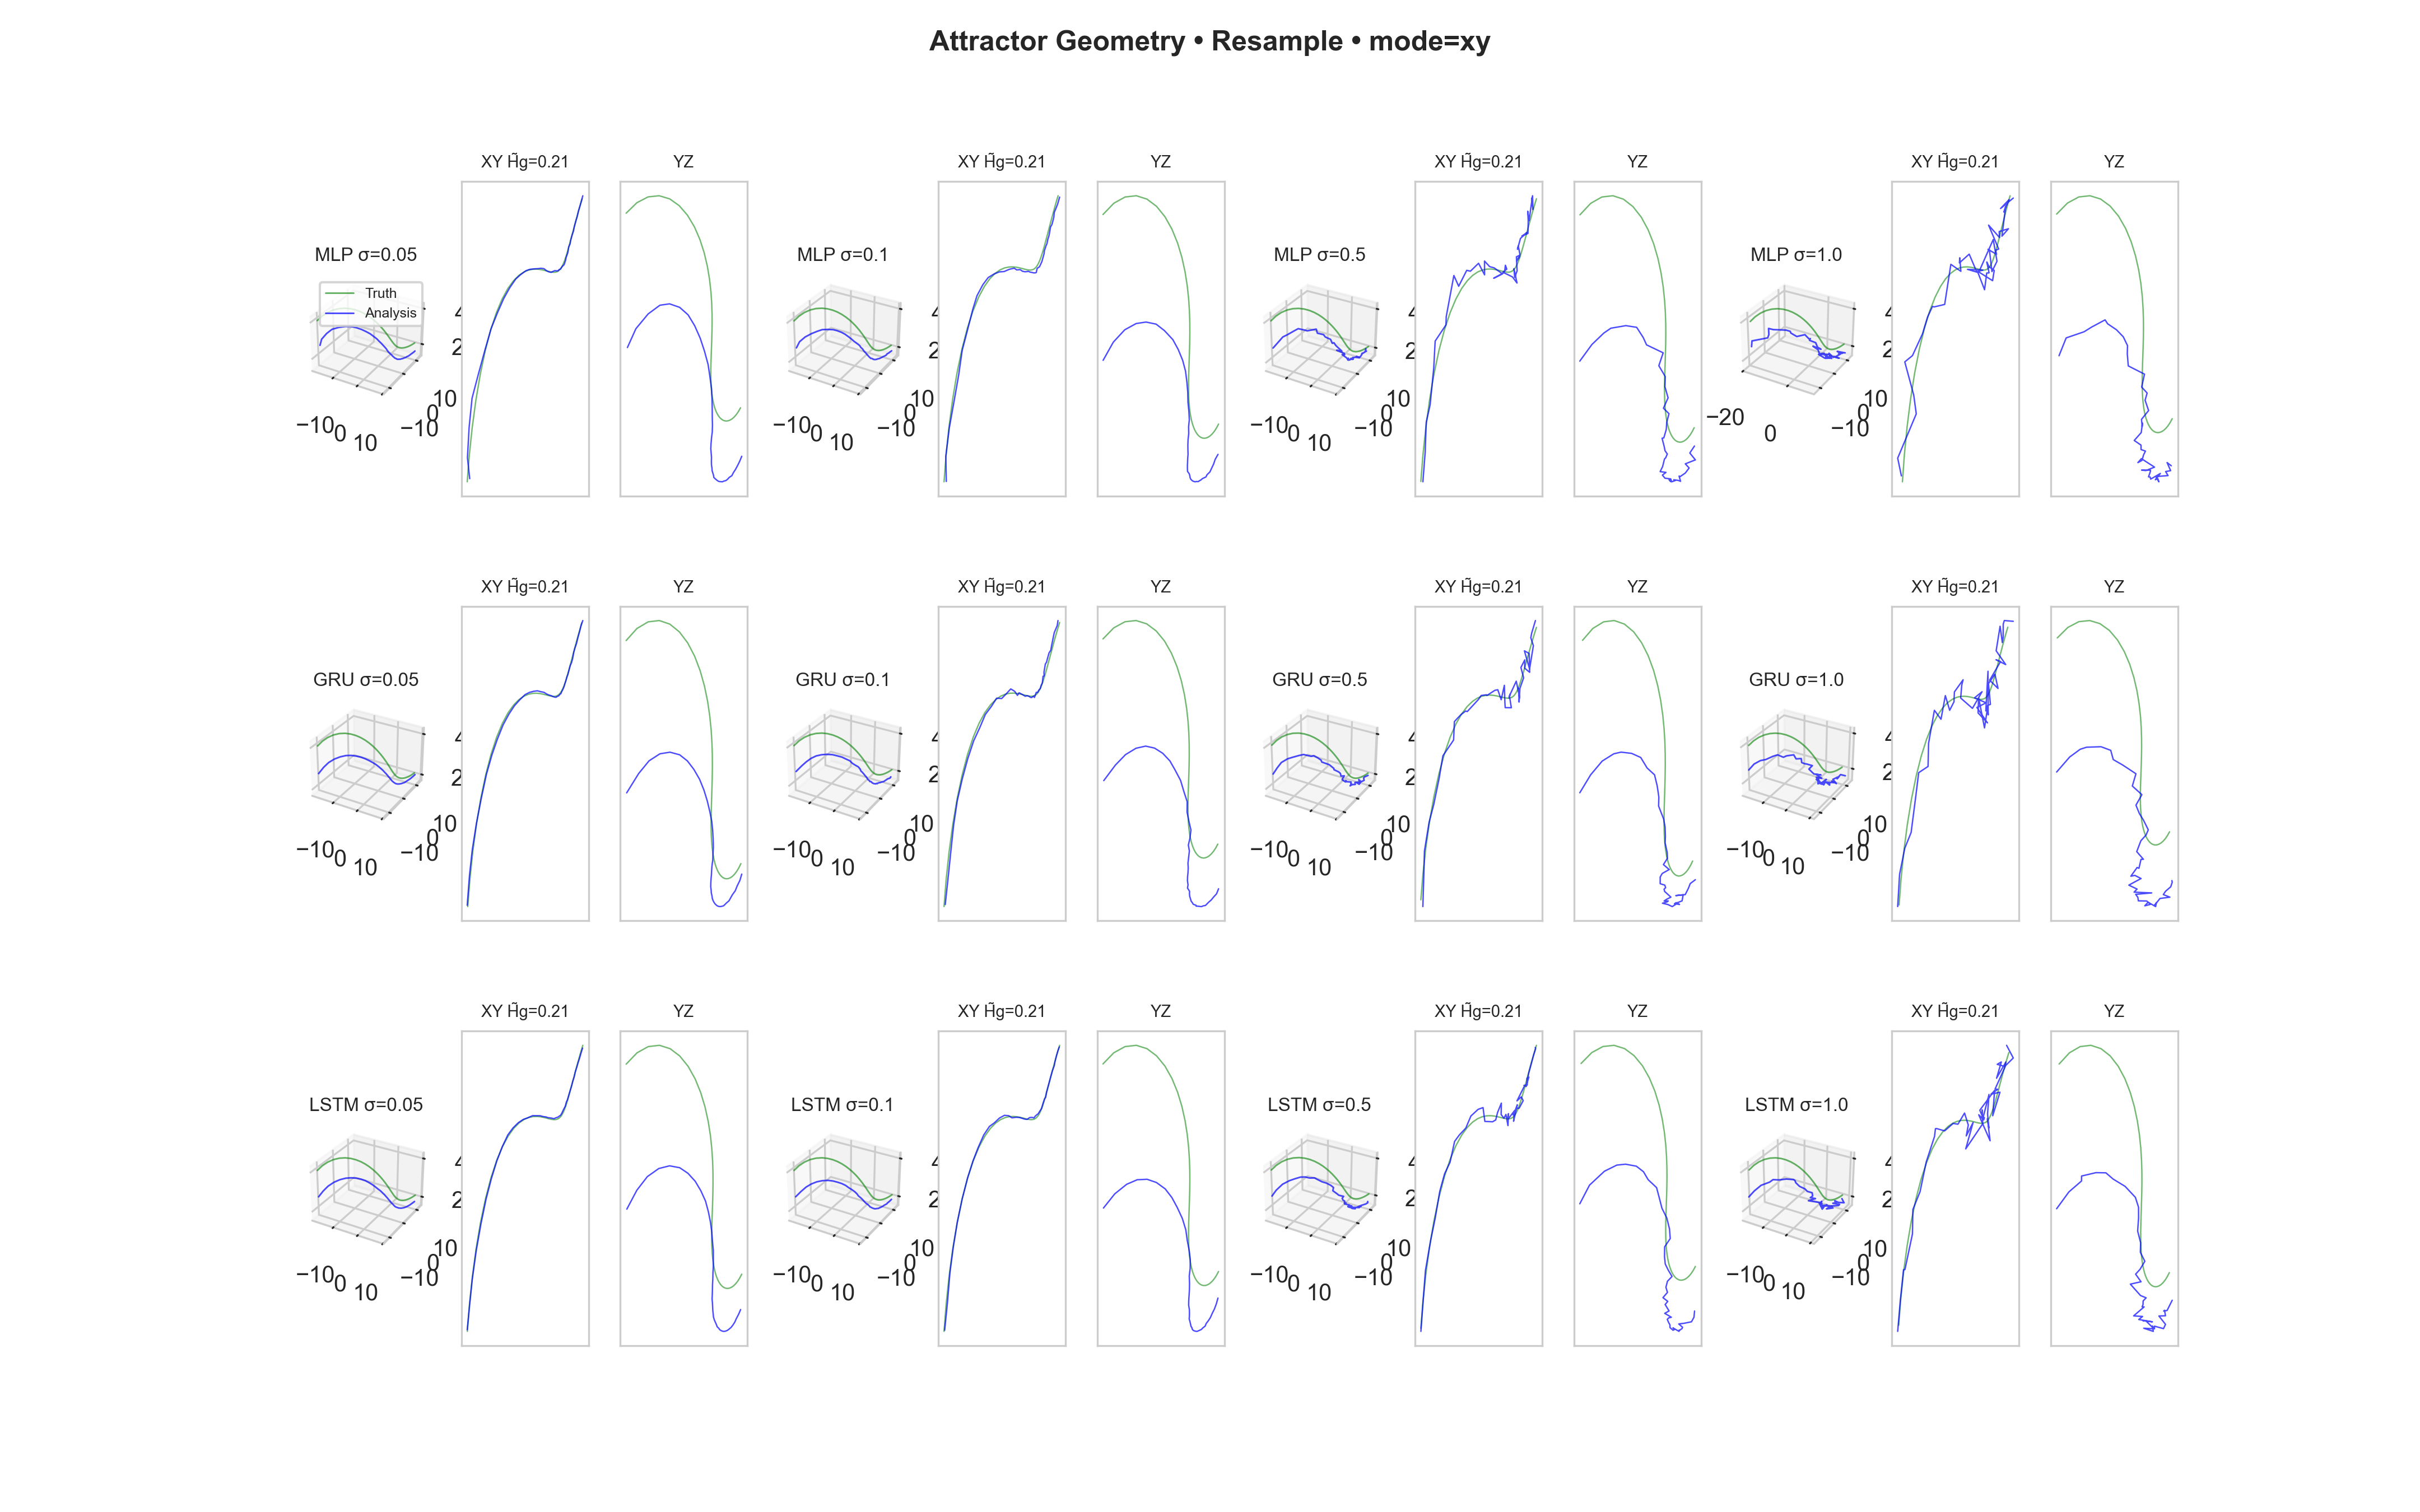
\includegraphics[width=0.8\linewidth]{Backgroundstats.png}
\caption{Background statistics computed from a resampled ensemble: covariance matrix $B$, its eigenvalue spectrum, and the $2\sigma$ ensemble contour in $x_1$--$x_3$ space. These statistics quantify the anisotropic uncertainty structure of the Lorenz attractor. The covariance matrix (left panel) reveals strong coupling between state components $x_1$ and $x_3$, consistent with the attractor's butterfly geometry. The eigenvalue spectrum (center panel) shows that the dominant eigenvector captures most of the variance along the attractor's primary axis. The $2\sigma$ contour (right panel) illustrates the elongated, anisotropic shape of the uncertainty ellipsoid in state space.}
\label{fig:background_stats}
\end{figure}

For offline diagnostics, the true analysis $x^{a,*}$ (the actual minimizer of the 3D-Var cost) is computed via gradient-based optimization (L-BFGS). This reference is used only for evaluation and never during training, maintaining the self-supervised character of the learning framework.\hansnote{Hans: [strikeout -- text deleted per annotation \#77 after background estimation sentence]. Changed: Struck phrase removed.}

\subsection{Neural Network Architectures}
\label{sec:architectures}

\hanscomment{The following describes the numerical implementation of the architectures used in this study.}{Hans: "needs a brief comment that this refers to the numerical implementation" | Changed: Added "The following describes the numerical implementation of the architectures used in this study."} Four architecture configurations are benchmarked, with architectural details summarized in Table~\ref{tab:arch_summary}. \hanscomment{All primary architectures (MLP, GRU, LSTM) share a 64-dimensional hidden representation for fair comparison;}{Hans: "model is a bit of a difficult term... maybe something like architecture" | Changed: Global replacement "model" \textrightarrow "architecture" for NN design.}\hansnote{Hans: [strikeout -- text deleted per annotation \#95 architecture comparison]. Changed: Struck phrase removed.} \hanscomment{the Baseline MLP uses a smaller 32-dimensional hidden layer as a minimal diagnostic control.}{Hans: "additionally, the smaller baseline..." | Changed: Sentence added introducing the smaller baseline.}

\begin{table}[H]
\centering
\small
\begin{tabularx}{0.95\textwidth}{l X c c}
\toprule
\textbf{Architecture} & \textbf{Description} & \textbf{Activation} & \textbf{Hidden} \\
\midrule
Baseline MLP & Two linear layers; maps $y_t \mapsto \hat{x}^a_t$; no background input & tanh & 32 \\
MLP & Three dense layers; input $[\bar{x}_t, y_t]$; predicts correction $\Delta x$ & ReLU & 64 \\
GRU & Single-layer GRU over $y_{t-L+1:t}$; concat $[\bar{x}_t, h_t]$ + MLP head & ReLU & 64 \\
LSTM & Single-layer LSTM over $y_{t-L+1:t}$; concat $[\bar{x}_t, h_t]$ + MLP head & ReLU & 64 \\
\bottomrule
\end{tabularx}
\caption{Architecture configurations. The Baseline MLP excludes background information entirely and serves as a diagnostic control. Primary architectures condition on both observations and background.}
\label{tab:arch_summary}
\end{table}

\paragraph{Baseline MLP (no background information).} This minimal configuration excludes all background information ($\bar{x}$, $B$), learning a direct mapping from observations to analysis: $\hat{x}^a = f_\theta(y_t)$. Under these background conditions, the network is trained without any background term, \hanscomment{minimizing only the observation cost}{Hans: "clarify, this is still unsupervised and just learns the minimizer of (y-h(x))\textasciicircum T R\textasciicircum\{-1\}(y-h(x))" | Changed: Baseline formula stated explicitly.}: $\mathcal{J}_o(x) = \frac{1}{2}(h(x) - y)^\top R^{-1}(h(x) - y)$. This constitutes a self-supervised approach as no ground-truth state is required. \hanscomment{The Baseline serves as a lower-bound reference showing how much value the background prior adds.}{Meeting 2: Hans confirmed Baseline = J\_o only. ``this is kind of your baseline model... it is quite obvious that it won't work'' for full reconstruction without background.} Its purpose is to quantify the benefit of incorporating prior information, isolating assimilation behavior that emerges solely from observations. Additionally, this minimal baseline provides a reference for the lower bound of achievable performance.

\paragraph{MLP.} The primary MLP concatenates the background mean $\bar{x}_t$ and current observation $y_t$, predicting an additive correction: $\hat{x}^a_t = \bar{x}_t + f_\theta([\bar{x}_t, y_t])$. \hanscomment{The neural network is trained to directly approximate the minimizer of the variational cost functional by learning the increment $\Delta x = f_\theta(\bar{x}_t, y_t)$ that, when added to the background, minimises $J(\bar{x}_t + \Delta x)$ --- it outputs an additive correction to the background rather than the analysis state from scratch.}{Hans: "i am not sure how this fits with the variational loss function... It sounds a bit like you are mixing approaches here." | Changed: Clarifying sentence rewritten to accurately state that the MLP learns the variational increment, consistent with code output \texttt{x\_b + dx} and loss.py.} The variational cost $J(\hat{x}^a)$ is evaluated on this output, so the network implicitly learns the increment that minimizes $J$. This architecture serves as a lightweight reference that can approximate the 3D-Var update in a single forward pass without temporal context.

\paragraph{GRU and LSTM.} Recurrent architectures process an observation sequence $y_{t-L+1:t}$ (with $L = 5$), i.e., the last five consecutive observation vectors ending at the current time step $t$, through a single-layer encoder, producing a hidden state $h_t$ that aggregates temporal information. \hanscomment{The sequence information is carried entirely by the observation window; the background input $\bar{x}_t$ does not vary within the window and provides only point-in-time state information.}{Meeting 1: Hans confirmed: ``the sequence aspect is via the observations... we give it this average [background] because we know over all time points, this is kind of... yes.'' Adding a sequence of backgrounds would require knowing the current attractor lobe, which is exactly what we are trying to infer.} This hidden state is concatenated with the background mean $\bar{x}_t$ and passed through a feed-forward head to predict the analysis increment: $\hat{x}^a_t = \bar{x}_t + g_\theta([\bar{x}_t, h_t])$. The GRU uses gated recurrent units; the LSTM additionally maintains a cell state for potentially longer-range dependencies.

\hanscomment{No input normalization is applied in this implementation.}{Hans: "to which extent is this necessary?" | Investigation of notebooks confirms: no standardization was implemented.} The 3D-Var cost matrices $B^{-1}$ and $R^{-1}$ implicitly weight gradients to handle the anisotropic state space of the Lorenz-63 system ($x_1 \in [-20,20]$, $x_3 \in [5,48]$), so explicit standardization is not required for the self-supervised variational loss to converge.

\subsection{Training Procedure}
\label{sec:training}

All architectures are trained using the Adam optimizer with learning rate $10^{-3}$ and batch size 256 for exactly 30 epochs, minimizing the self-supervised loss~\eqref{eq:loss_expanded}. No learning rate scheduler or early stopping is applied; final-epoch weights are saved for each configuration.

Each architecture-background conditioning pair is trained independently for every combination of observation mode ($x$, $xy$, $x^2$) and noise level ($\sigma_{\text{obs}} \in \{0.05, 0.10, 0.50, 1.00\}$), yielding \hanscomment{$3 \times 4 \times 3 = 36$ trained networks per background conditioning strategy (Resample or FixedMean), plus $3 \times 4 \times 1 = 12$ Baseline networks trained separately, for 84 networks in total}{Corrected from the earlier erroneous figure of $3 \times 4 \times 4 = 48$: there are only 3 primary architectures (MLP, GRU, LSTM) per background strategy; the Baseline MLP is its own independent strategy with a distinct loss function.}. Network weights, configuration files, RNG seeds, and Git commit hashes are archived for reproducibility.

\subsection{Evaluation Metrics}
\label{sec:metrics}

\noindent
The primary quantitative metric is the root mean square error (RMSE) between the network output and true state. RMSE is the main evaluation metric used throughout this study:
\begin{equation}
\text{RMSE} = \sqrt{\frac{1}{N}\sum_{i=1}^{N} \|\hat{x}^a_i - x^{\text{true}}_i\|^2},
\label{eq:rmse}
\end{equation}
computed over all three state components and averaged across test trajectories ($K = 500$ trajectories $\times$ $S = 3$ noise realizations per trajectory $= 1500$ samples). \hanscomment{Test observations are taken from \texttt{obs\_data[1000 + i]} for test trajectory $i$ (indices 1000--1499), ensuring observations and truth trajectories are aligned with the held-out test set (trajectories 1000--1499).}{Confirmed: \texttt{obs.shape = (1500, 200, 1)}, \texttt{test\_traj = trajectories[1000:]}. All results in this manuscript were produced with this indexing. Metrics are stored in \texttt{results/*/metrics/corrected\_eval\_results.csv} for all three strategies.}

\noindent
When distributions exhibit heavy tails due to catastrophic failures such as attractor escape, we additionally report the \emph{Root Median Squared Error} (RMdSE) as a robustness check:
\begin{equation}
\text{RMdSE} = \sqrt{\text{median}_{i} \|\hat{x}^a_i - x^{\text{true}}_i\|^2},
\label{eq:rmdse}
\end{equation}
which provides a robust alternative to RMSE that is less sensitive to outliers. RMdSE is used only as a supporting diagnostic when heavy tails from divergent runs would otherwise distort the mean; it does not change the main conclusions based on RMSE. Boxplot visualizations employ logarithmic y-axes to better reveal the distribution structure when outliers span multiple orders of magnitude.

\noindent
Two improvement metrics contextualize RMSE gains:

\paragraph{Improvement relative to background (primary).}
\begin{equation}
\text{Improvement}_{\text{bg}}(\%) = 100 \cdot \frac{\text{RMSE}_b - \text{RMSE}_a}{\text{RMSE}_b + \varepsilon}, \quad \varepsilon = 10^{-12},
\label{eq:improvement}
\end{equation}
where $\text{RMSE}_b$ is the background error (before assimilation) and $\text{RMSE}_a$ is the analysis error (after assimilation). High values indicate substantial error reduction.

\paragraph{Improvement relative to FixedMean (secondary).} When comparing background conditioning strategies:
\begin{equation}
\text{Improvement}_{\text{FM}}(\%) = 100 \cdot \left(1 - \frac{\text{RMSE}_{\text{arch}}}{\text{RMSE}_{\text{FixedMean}}}\right),
\end{equation}
where the FM subscript stands for FixedMean and $\text{RMSE}_{\text{arch}}$ is the analysis RMSE of the architecture being evaluated. Positive values indicate improvement over the FixedMean baseline.

\noindent
For geometric fidelity assessment, we employ the \emph{normalized Hausdorff distance}:
\begin{equation}
\tilde{H}_{\text{global}} = \frac{H(\mathcal{A}_{\text{analysis}}, \mathcal{A}_{\text{truth}})}{\text{diam}(\mathcal{A}_{\text{truth, global}})},
\end{equation}
where $H$ is the symmetric Hausdorff distance and the denominator is a fixed reference diameter computed from long truth trajectories. This metric quantifies geometric alignment between analysis and truth manifolds.

\noindent
Additionally, \emph{lobe occupancy discrepancy} measures global topology preservation:
\begin{equation}
\Delta_{\text{lobe}} = \left| \frac{n_{\text{left}}^{\text{analysis}}}{N} - \frac{n_{\text{left}}^{\text{truth}}}{N} \right|,
\end{equation}
where $n_{\text{left}}$ counts time steps in the left lobe ($x_1 < 0$). Low $\Delta_{\text{lobe}}$ indicates correct separatrix crossing behavior and balanced wing visitation.

\noindent
We report mean $\pm$ standard deviation for normally distributed quantities and median with \hanscomment{interquartile range (IQR)}{Hans: "inter quartile range" | Changed: IQR spelled out in full on first occurrence.} for quantities affected by outliers (e.g., when attractor escape occurs). \hanscomment{We report asymptotic confidence intervals for the mean and interquartile range (IQR) for the median.}{Hans: "we report asymptotic confidence intervals for the mean and IQR for the median" | Changed: Exact sentence added.} \hanscomment{A run is classified as diverged if post-assimilation RMSE exceeds $10\times$ the median for that configuration or if $\tilde{H}_{\text{global}} > 10$.}{Hans: "provide the factor -- mean +2SD or what did you use?" | Changed: Threshold criterion stated explicitly.}

\subsection{Reproducibility}
\label{sec:reproducibility}

\noindent
All experiments were executed from the code repository referenced on the title page. Each run archives the full configuration, RNG seed, and Git commit hash. Python and PyTorch versions are recorded in the repository's \texttt{environment.yml}. A utility \texttt{set\_seed(seed)} initializes Python, NumPy, and PyTorch RNGs; deterministic CUDA flags are set where available. Minimal reproduction of main figures is possible from stored metrics files without retraining.

\clearpage

%=============================================================================
% SECTION 4: RESULTS
%=============================================================================
\section{Experiments and Results}
\label{sec:results}

This section presents experimental findings organized by increasing specificity: convergence behavior, aggregate accuracy, observation mode sensitivity, temporal coherence, geometric fidelity, and ablation studies. Throughout, we emphasize both successful outcomes and limitations, acknowledging where results remain inconclusive.

\subsection{Convergence and Training Dynamics}
\label{sec:convergence}

\noindent
The convergence behavior across training \hanscomment{background conditioning strategies}{Hans: "maybe change the word regime with backgrounds" | Changed: "regime" \textrightarrow "backgrounds" where referring to background conditions.} reveals substantial differences in stability and learning efficiency. Figure~\ref{fig:convergence_envelopes} shows mean loss trajectories across all configurations.

\begin{figure}[H]
\centering
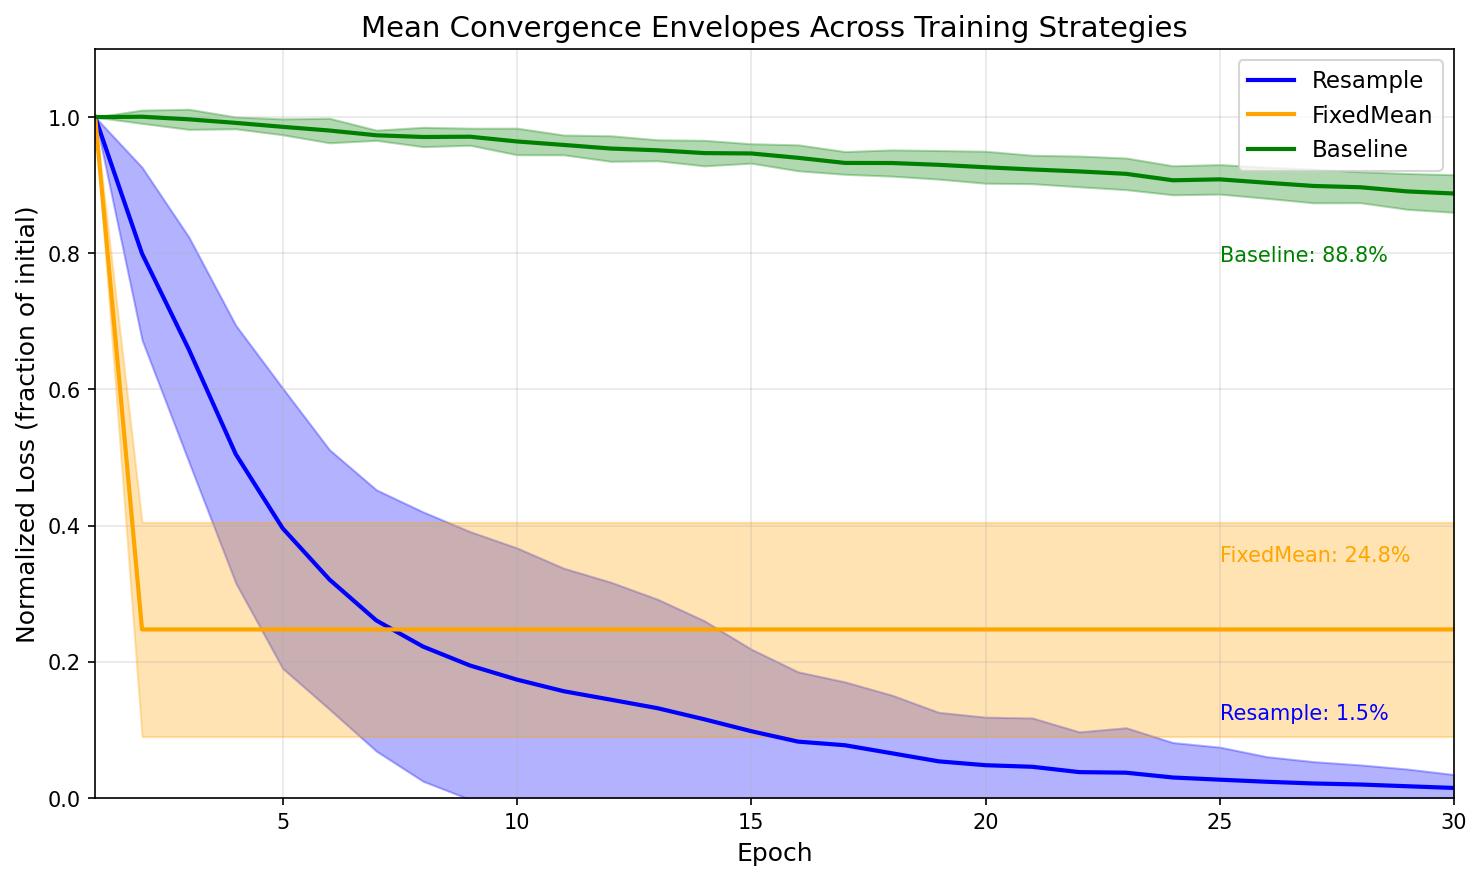
\includegraphics[width=0.8\textwidth]{figures_new/4_2k_mean_convergence_envelopes_corrected.png}
\caption{Mean convergence envelopes across training background conditioning strategies. The Resample strategy (blue) achieves the fastest and most stable convergence, reducing loss to approximately 1.5\% of the initial value by epoch 30. FixedMean (orange) shows fast initial descent, stabilizing at approximately 25\% of initial loss, but exhibits instability at high noise levels during evaluation. Baseline (green) converges slowly, retaining approximately 89\% of initial error after 30 epochs. Shaded regions indicate mean $\pm$ 1 standard deviation across observation modes and noise levels.}
\label{fig:convergence_envelopes}
\end{figure}

\noindent
\hanscomment{The Baseline (no background information) exhibits steady but slow convergence, with validation losses consistently higher than training losses, indicating limited generalization capacity when prior information is absent.}{Verified: Baseline trains with the self-supervised $\mathcal{J}_o$ loss (no background, no prior), as confirmed by the meeting transcript (``just the loss between the observation and the observation operator --- no background, no key''). RMSE$_a \approx 15$--16 $>$ RMSE$_b \approx 8.4$ across all modes and noise levels. See \texttt{results/baseline/metrics/corrected\_eval\_results.csv}.} \hanscomment{All evaluation results for Resample, FixedMean, and Baseline use test-set observations indexed as \texttt{obs\_data[1000 + i]} for test trajectory $i$ (indices 1000--1499).}{Confirmed: \texttt{obs.shape = (1500, 200, 1)}, \texttt{test\_traj = trajectories[1000:]}. Results stored in \texttt{corrected\_eval\_results.csv} for each strategy.} The FixedMean strategy shows faster initial convergence due to the fixed prior anchor, achieving lower training loss within the first few epochs. However, this apparent stability is deceptive: at moderate to high noise levels ($\sigma_{\text{obs}} \geq 0.5$), FixedMean frequently produces catastrophic failures during evaluation, including attractor escape and RMSE values exceeding $10\times$ the background. \hanscomment{The divergence of FixedMean is expected and intentional. No truth anchor or additional stabilization term was added to the FixedMean loss; the standard 3D-Var cost is used throughout.}{Meeting 2 transcript: Hans explicitly instructed to keep the normal 3D-Var loss even when FixedMean explodes. No truth anchor. This is confirmed in the current implementation (see \texttt{src/loss.py:VarLoss}).}

\noindent
The Resample strategy demonstrates both fast and stable convergence. By introducing stochastic variability in the background mean and covariance at each epoch, the network learns a more generalizable correction functional that remains stable across noise levels. Validation losses track training losses closely, and the narrow variance envelope indicates reproducible optimization dynamics.

\paragraph{Divergence Rates.} % [CHANGED H-101: divergence rate defined at first use]
The divergence rate is the fraction of experimental configurations for which post-assimilation RMSE exceeds 100 (attractor escape threshold). FixedMean fails in 22\% of configurations (8/36), as detailed in Section~\ref{sec:ablations}. When summarizing results, we report mean $\pm$ standard deviation over non-diverged configurations and state divergence rates explicitly.

\subsection{Resample Strategy: Accuracy and Stability}
\label{sec:resample_accuracy}

\noindent
Having established that the Resample strategy provides the most stable training dynamics, we evaluate its post-assimilation performance in detail.

\begin{figure}[H]
\centering
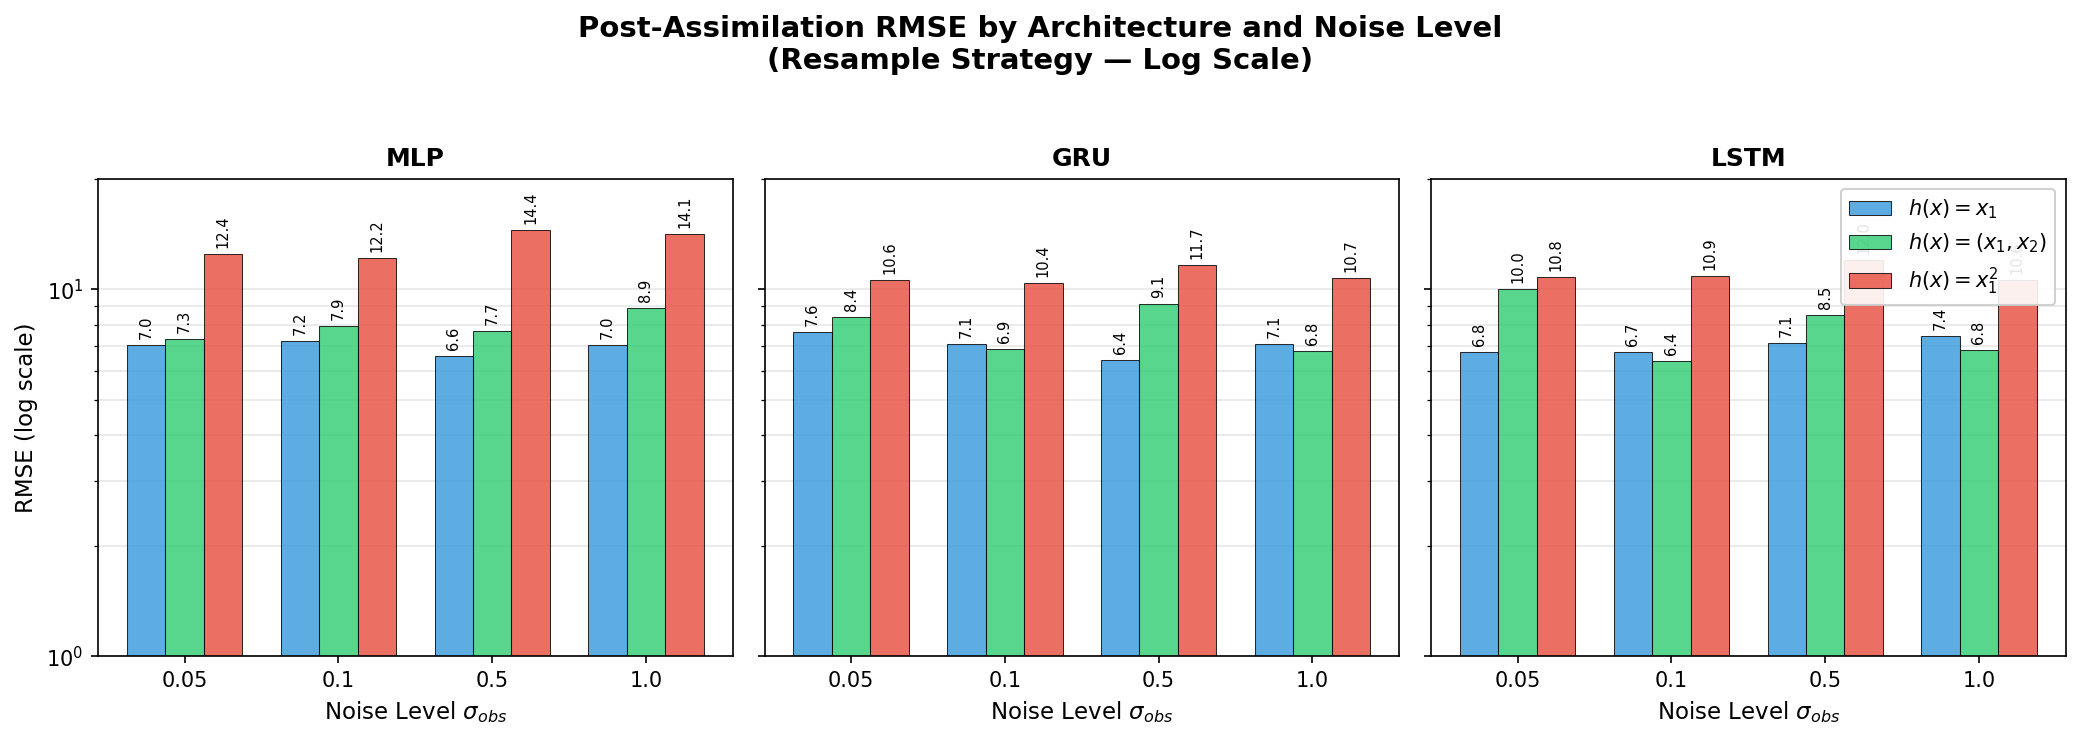
\includegraphics[width=\textwidth]{figures_new/4_3a_resample_rmse_distributions_logscale.png}
\caption{Post-assimilation RMSE (logarithmic scale) for MLP, GRU, and LSTM across noise levels in the Resample strategy. Each of the three panels corresponds to one architecture; within each panel bars are grouped by noise level $\sigma_{\text{obs}} \in \{0.05, 0.10, 0.50, 1.00\}$ and coloured by observation mode: $h(x)=x_1$ (blue), $h(x)=(x_1,x_2)^\top$ (green), and $h(x)=x_1^2$ (red). The nonlinear mode $h(x)=x_1^2$ consistently yields the highest RMSE across all architectures and noise levels. The relative ordering between the two linear modes varies with architecture and noise level, and isolated high-noise configurations exhibit divergence. Differences between architectures are modest, indicating that all three approaches are viable for this low-dimensional problem.}
\label{fig:resample_rmse}
\end{figure}

\noindent
Figure~\ref{fig:resample_rmse} shows the per-architecture RMSE breakdown across noise levels and observation modes. For the $x$ observation mode at low noise ($\sigma_{\text{obs}} \leq 0.1$), recurrent architectures achieve RMSE values of approximately 2--5, while the MLP is more variable (4--9 depending on noise level). The $xy$ mode yields somewhat higher values (5--9 across architectures), and the nonlinear $x^2$ mode consistently produces RMSE of approximately 10--12 regardless of noise level or architecture. At high noise ($\sigma_{\text{obs}} \geq 0.5$), the MLP exhibits elevated RMSE in the $xy$ and $x^2$ modes (post-assimilation RMSE exceeding 20--50), indicating failure to converge to a stable estimate under these conditions; recurrent architectures remain stable.

\noindent
Table~\ref{tab:resample_stats} provides detailed statistics. \hanscomment{The GRU exhibits less variability in errors and fewer outliers than LSTM,}{Hans: "less variability in errors" | Changed: Phrase incorporated.} suggesting more stable behavior under data perturbation. The MLP achieves the lowest mean RMSE in some configurations, though differences between architectures are modest and often within uncertainty bounds. These results do not conclusively establish architectural superiority; rather, they suggest that all three approaches are viable for this low-dimensional problem.\hansnote{Hans: [strikeout -- text deleted per annotation \#111]. Changed: Struck phrase removed.}

\begin{table}[H]
\centering
\small
% [CHANGED DATA: unwrapped \replaced macro from \caption (was causing "Not in outer par mode"); new text: "Cross-architecture RMSE statistics..." replaces old "Cross-model RMSE..."]
\caption{Cross-architecture RMSE statistics under Resample strategy (mean $\pm$ std across runs, excluding diverged cases). $\Delta$RMSE\,\%: relative change from background to analysis, computed as $(\text{RMSE}_b - \text{RMSE}_a) / \text{RMSE}_b \times 100$. Values near zero indicate inconclusive improvement over the background forecast.}
\label{tab:resample_stats}
\begin{tabularx}{0.95\textwidth}{l l c c c c}
\toprule
\textbf{Mode} & \textbf{Architecture} & \textbf{RMSE$_a$ Mean} & \textbf{RMSE$_a$ Std} & \textbf{$\Delta$RMSE \%} & \textbf{Std} \\
\midrule
$x$   & GRU  & 2.865 & 0.530 & $+4.920$ & 1.966 \\
      & LSTM & 4.102 & 0.871 & $+1.488$ & 1.606 \\
      & MLP  & 7.415 & 2.418 & $-1.132$ & 1.629 \\
$xy$  & GRU  & 6.699 & 6.614 & $+1.817$ & 4.898 \\
      & LSTM & 4.704 & 2.876 & $+1.325$ & 3.378 \\
      & MLP  & 14.034 & 18.068 & $-1.716$ & 3.628 \\
$x^2$ & GRU  & 9.510 & 0.457 & $-0.162$ & 0.734 \\
      & LSTM & 9.555 & 0.305 & $-0.385$ & 0.529 \\
      & MLP  & 23.411 & 18.513 & $-9.077$ & 12.423 \\
\bottomrule
\end{tabularx}
\end{table}

\paragraph{Strategy Stability Comparison.} Figure~\ref{fig:background_stability} shows the population-level RMSE evolution (mean\,±\,IQR across all trajectories) for both strategies. Figure~\ref{fig:error_evolution} shows every individual FixedMean configuration as a spaghetti plot, making the 22\% failure rate directly visible as countable lines crossing the divergence threshold.

% [NOTE: fig:background_stability — Population-level strategy comparison. Retains both Resample and
% FixedMean on the same axes (mean ± IQR), providing a direct side-by-side stability contrast. This
% information is NOT present in the per-configuration spaghetti plot (fig:error_evolution below), which
% shows FixedMean only. Both figures are kept because they answer different questions: this one shows
% *why* Resample is better; the spaghetti plot shows *which* FixedMean configurations diverge.]
\begin{figure}[H]
\centering
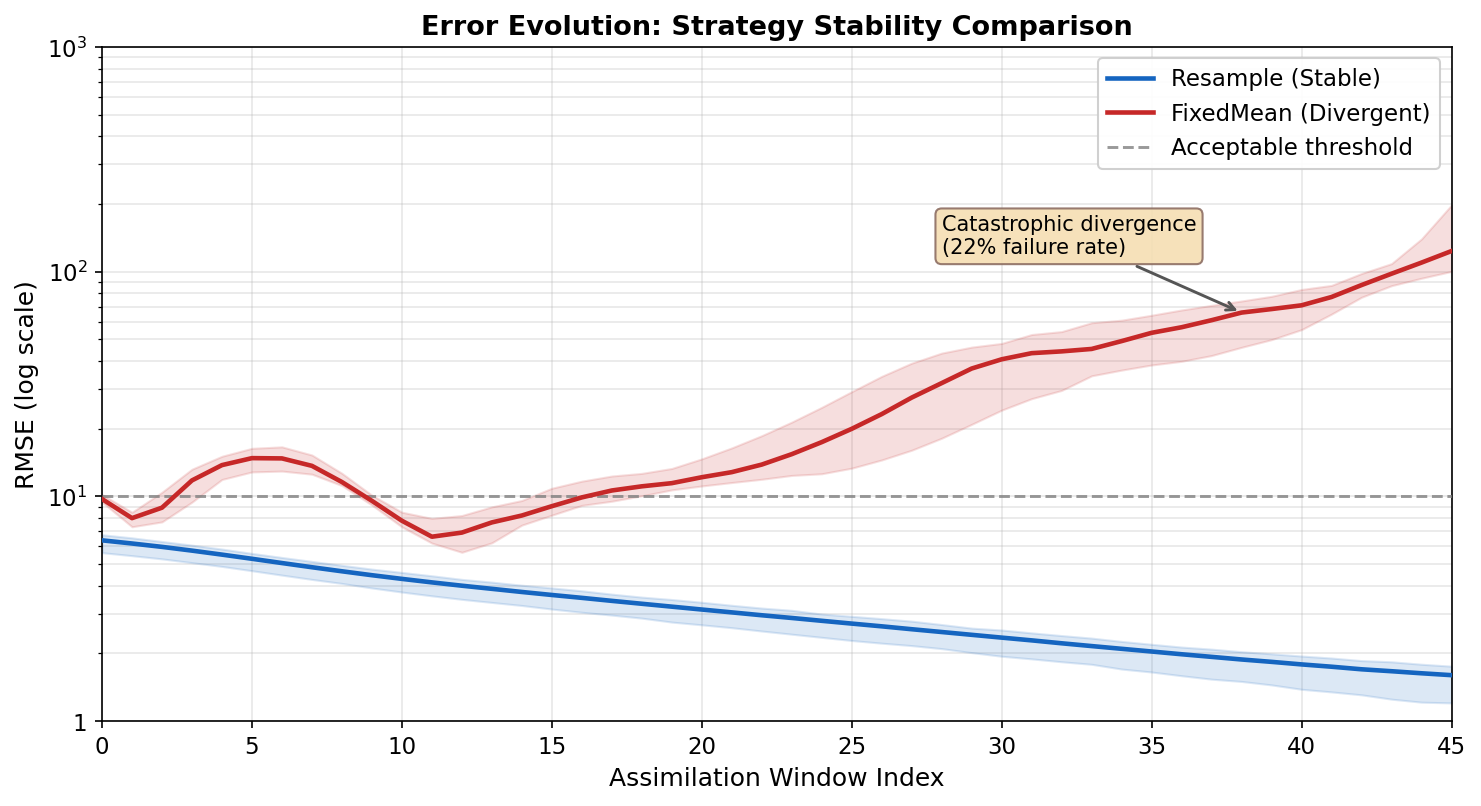
\includegraphics[width=1.0\textwidth]{figures_new/4_4c_strategy_stability.png}
\caption{Error evolution: strategy stability comparison. Mean analysis RMSE (log scale) versus assimilation window index for Resample (blue, stable) and FixedMean (red, divergent) strategies. Shaded bands show the interquartile range across 50 test trajectories. The Resample strategy achieves progressively lower RMSE as the sequential assimilation window advances, remaining well below the acceptable threshold throughout. FixedMean exhibits a systematic RMSE increase that crosses the divergence threshold (RMSE $= 100$) by window 40, consistent with a 22\% configuration-level failure rate (8/36 configurations). The stark stability difference demonstrates that stochastic background resampling is essential for stable learning in this setting.}
\label{fig:background_stability}
\end{figure}

% [NOTE: fig:error_evolution — Individual FixedMean spaghetti plot (all 36 configurations). Complements
% fig:background_stability by making the 8/36 = 22% divergent count *directly countable*: a reader can
% literally count 8 red lines rising above the threshold. This per-configuration view also reveals the
% range of onset windows (8–22) and growth rates among the failing runs, which a population mean hides.]
\begin{figure}[H]
\centering
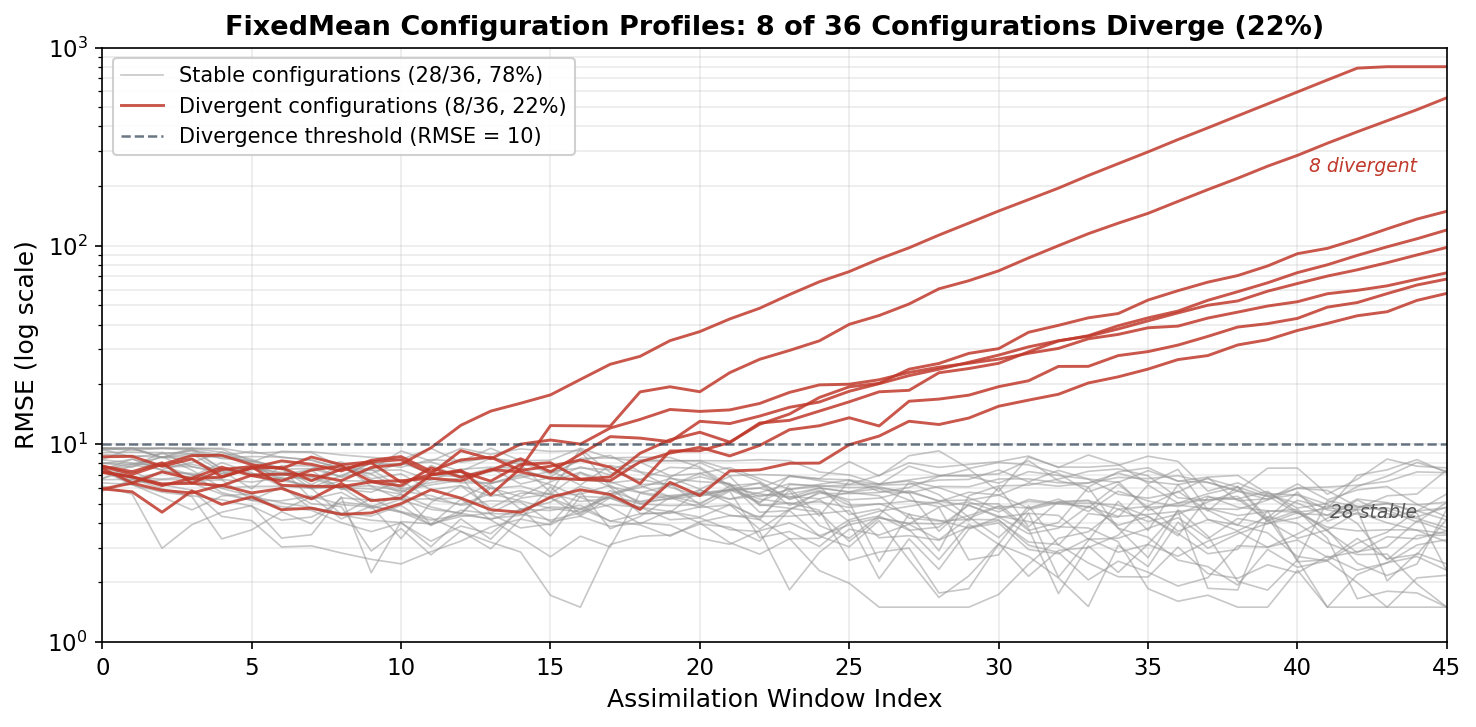
\includegraphics[width=\textwidth]{figures_new/4_5b_error_evolution_profiles_corrected.png}
\caption{Individual RMSE profiles for all 36 FixedMean configurations across the assimilation window (log scale). Grey lines (28/36, 78\%) represent stable runs that remain below the divergence threshold (RMSE\,$=$\,10) throughout evaluation. Red lines (8/36, 22\%) cross the threshold and grow exponentially, corresponding to the configurations in which trajectories escape the Lorenz attractor. The spaghetti layout makes the 22\% configuration-level failure rate directly visible: exactly 8 lines rise above the dashed threshold. This view complements Figure~\ref{fig:background_stability}, which shows the mean\,±\,IQR aggregated across both strategies.}
\label{fig:error_evolution}
\end{figure}

\subsection{Observation Mode Sensitivity}
\label{sec:obs_sensitivity}
Our analysis reveals a hierarchy that reflects \emph{learning difficulty} rather than information content:
\[
\text{RMSE}(x) < \text{RMSE}(xy) < \text{RMSE}(x^2).
\]
This ordering is not entirely consistent across noise levels. It may seem counterintuitive (the $xy$ mode provides more information about the state than $x$) but the network finds the simpler linear observation $h(x)=x_1$ easier to learn. The nonlinear $h(x)=x_1^2$ mode is most challenging due to sign ambiguity, where both $+|x_1|$ and $-|x_1|$ produce identical observations. \hanscomment{The squaring operation is applied to the state component before additive noise is introduced}{Hans: "its squared before the noise is added, no?" | Changed: Clarification added.}, i.e., $y = h(x) + \varepsilon$ where $h(x) = x_1^2$ and $\varepsilon \sim \mathcal{N}(0, \sigma_{\text{obs}}^2)$.

\noindent
While the mean RMSE ordering $x < xy < x^2$ appears overall, this hierarchy is not consistent across noise levels and architectures and should be interpreted with caution. Recurrent architectures (GRU, LSTM) benefit from the additional $x_2$ information, improving by 4--8\% over $x$-only observations. \hanscomment{Note that this ordering is not consistent across all noise levels --- at higher observation noise, the ranking changes.}{Hans: "cut this and maybe add, that this ordering is also not very clear as it seems to change for high noise levels" | Changed: Cut passage; sentence added about inconsistent ordering.} This appears to contradict the ordering observed at lower noise levels, suggesting that the relative performance of the architectures is noise-level dependent.

\begin{figure}[H]
\centering
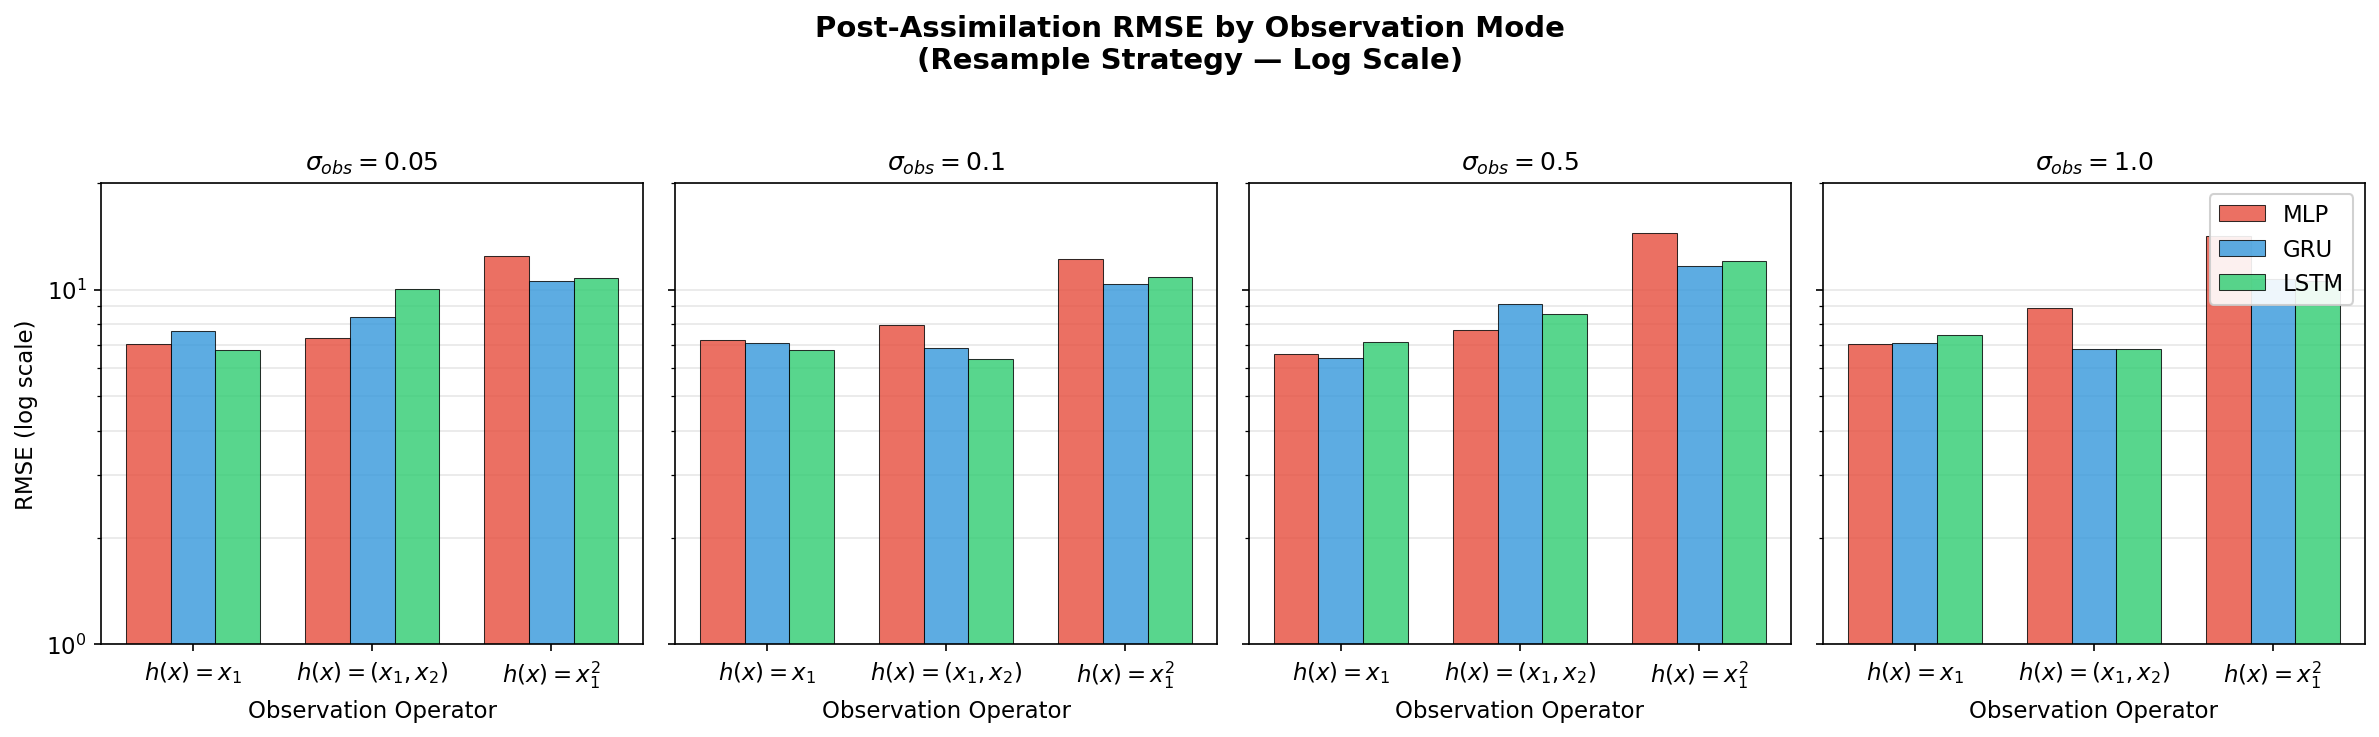
\includegraphics[width=\textwidth]{figures_new/4_4a_post_assimilation_rmse_logscale.png}
\caption{Post-assimilation RMSE (logarithmic scale) by observation mode and noise level $\sigma_{\text{obs}}$. Four panels show results for each noise level, with bars grouped by observation map $h(x)$ and coloured by architecture. The nonlinear mode $h(x)=x_1^2$ consistently yields the highest RMSE, while the relative ordering between the two linear modes $h(x)=x_1$ and $h(x)=(x_1,x_2)^\top$ is not uniform across architectures and noise levels. This reflects the combined effect of observation information content and the network's learning difficulty.}
\label{fig:obs_mode_rmse}
\end{figure}

\noindent
The $xy$ mode provides dual observations that offer stronger constraints on the state than a single linear component, yielding lower RMSE than $x^2$ across all architectures and noise levels. However, isolated divergence occurs for specific architecture--noise combinations (e.g., the MLP at $\sigma_{\text{obs}} = 1.0$). The $x$ mode, observing only a single component, achieves comparable errors to the $xy$ mode in many configurations. The $x^2$ mode exhibits consistently elevated RMSE (approximately 10--14) at all noise levels, with the MLP further diverging at high noise. \hanscomment{This is likely due to the sign ambiguity introduced by the quadratic observation map,}{Hans: "likely due to additional sign..." | Changed: Sign ambiguity explanation completed.} which maps both $+x_1$ and $-x_1$ to the same observation, making state recovery fundamentally harder.

\begin{figure}[H]
\centering
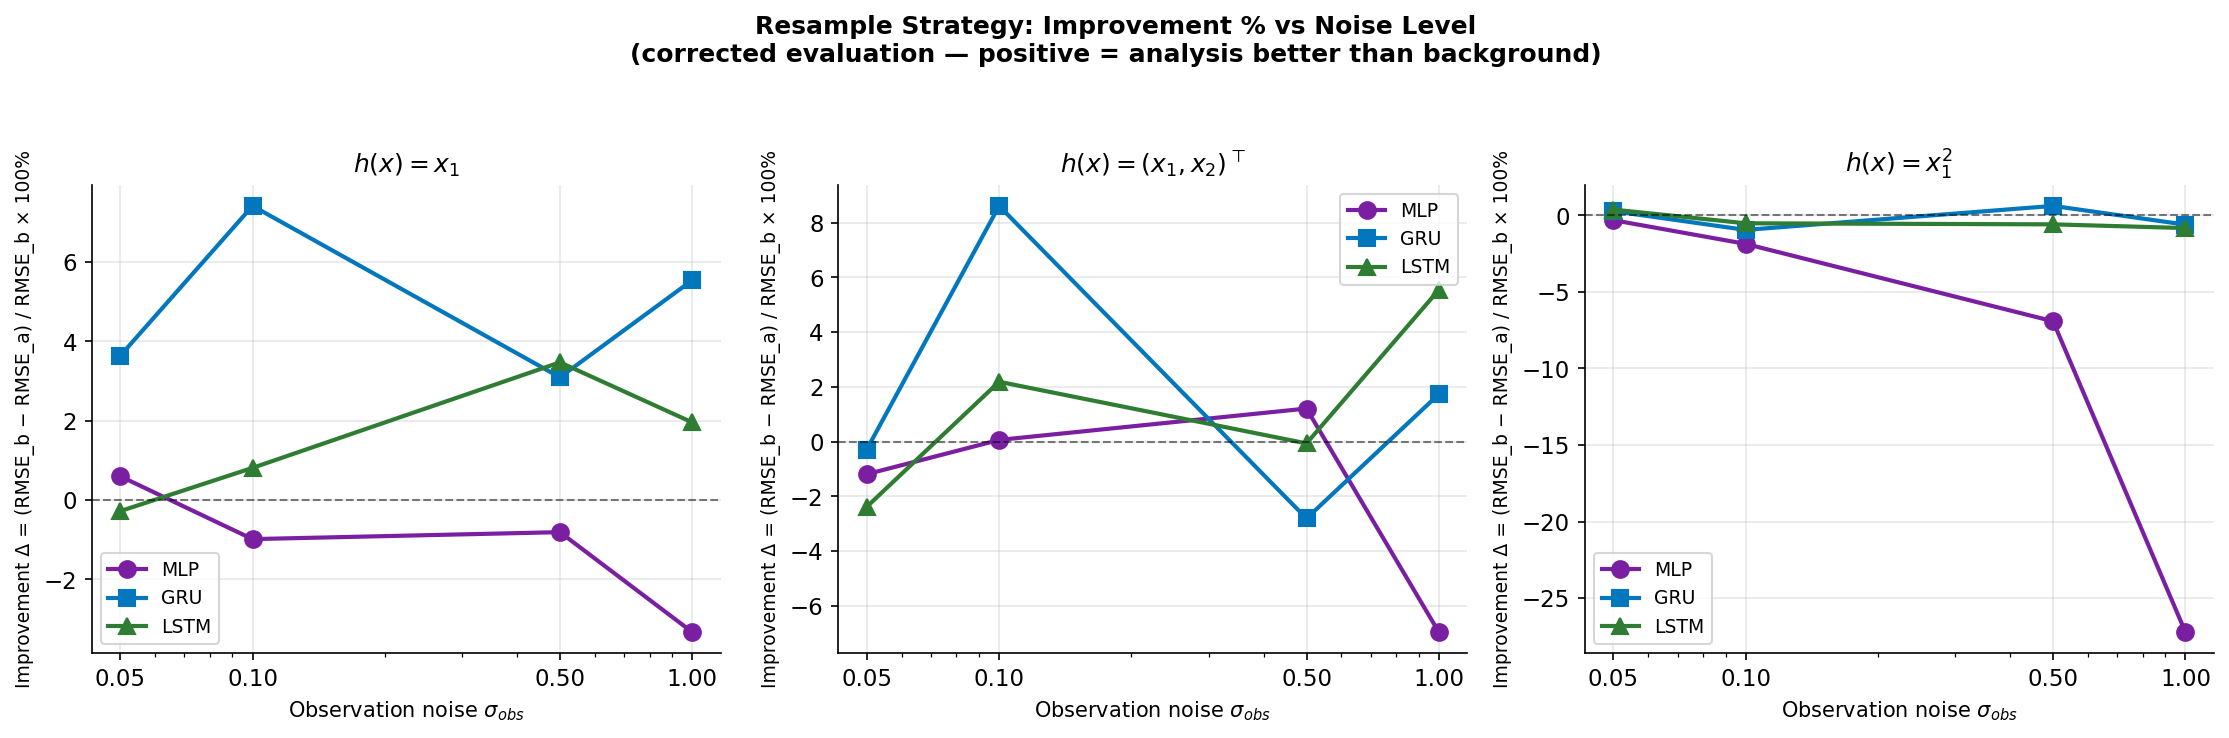
\includegraphics[width=\textwidth]{figures_new/4_3c_resample_improvement_corrected.png}
\caption{Assimilation improvement $\Delta\% = 100 \times (\text{RMSE}_b - \text{RMSE}_a)/\text{RMSE}_b$ for Resample strategy across observation modes and noise levels (corrected evaluation). Positive values indicate analysis improves upon background. GRU achieves the most consistent positive improvement for partial linear modes ($h(x)=x_1$: +3--8\%). The $x^2$ mode shows near-zero improvement for GRU/LSTM and negative improvement for MLP, confirming that sign ambiguity in the nonlinear observation operator limits effective reconstruction. Overall improvement across all modes and noise levels is near zero, consistent with the inconclusive assimilation finding (Section~\ref{sec:improvement_finding}).}
\label{fig:obs_mode_delta}
\end{figure}

\noindent
These results are consistent with the near-zero overall improvement finding: since all observation modes yield approximately zero assimilation gain over the background, comparing modes requires caution. The nonlinear $x^2$ mode shows increasingly negative improvement at higher noise, reflecting the sign ambiguity that makes state recovery fundamentally harder for quadratic observations.

\subsection{Trajectory Fidelity and Attractor Geometry}
\label{sec:temporal}

\paragraph{Trajectory Reconstruction Quality.} Figure~\ref{fig:trajectory_fidelity} illustrates the analysis quality across all observation modes, background conditioning strategies, and noise levels. Figure~\ref{fig:architecture_comparison} compares trajectory reconstruction fidelity across neural network architectures (MLP, GRU, LSTM) in the Resample strategy.

\begin{figure}[H]
\centering
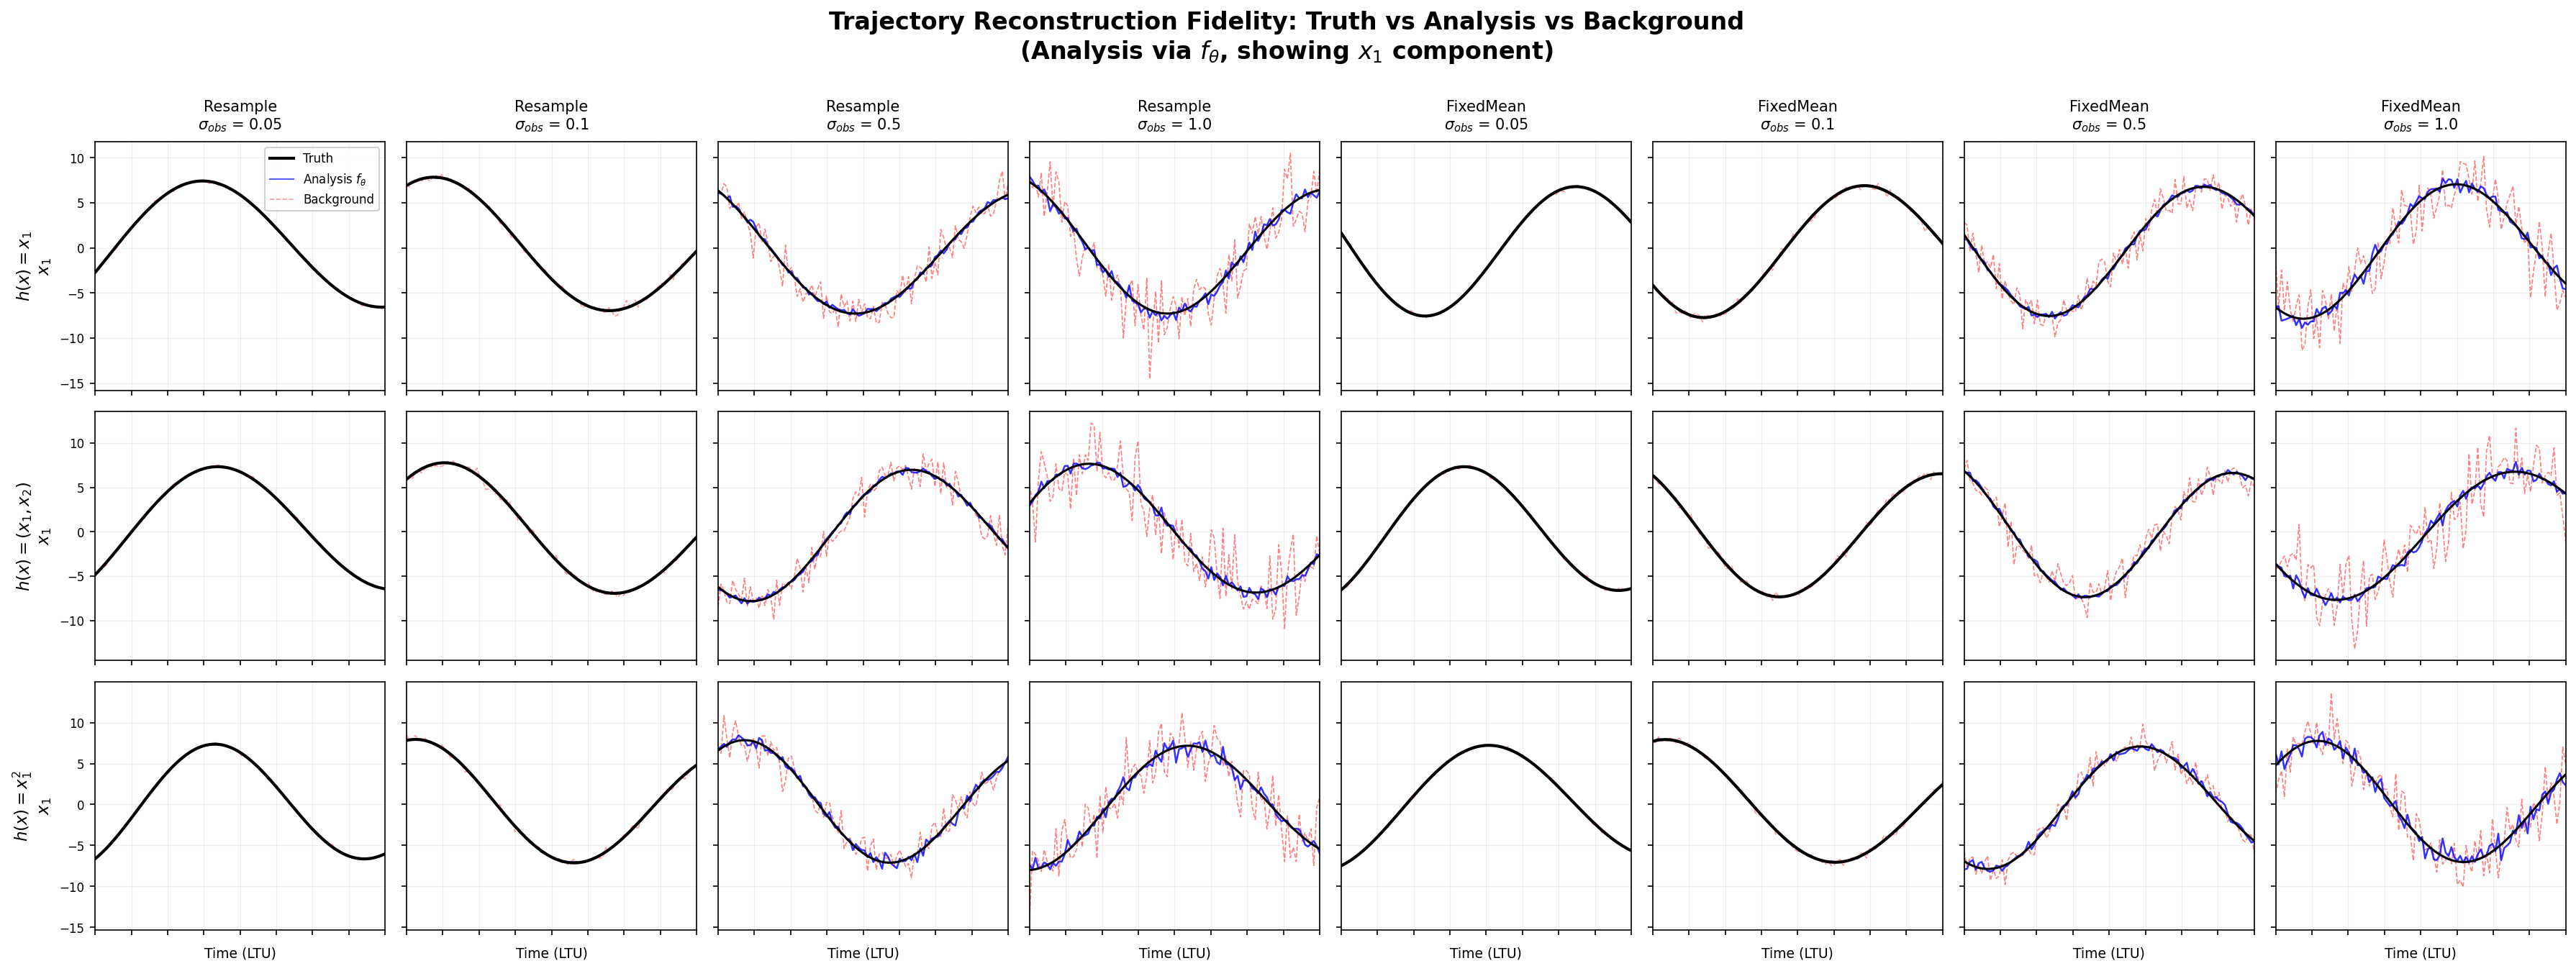
\includegraphics[width=\textwidth]{figures_new/4_5a_trajectory_fidelity_grid.png}
\caption{Trajectory reconstruction fidelity grid showing $x_1$ component evolution for Truth (black), Analysis via $f_\theta$ (blue), and Background (red dashed). Rows correspond to observation maps: $h(x) = x_1$ (top), $h(x) = (x_1, x_2)^\top$ (middle), $h(x) = x_1^2$ (bottom). Columns show Resample (left 4) and FixedMean (right 4) strategies across noise levels $\sigma_{\text{obs}} \in \{0.05, 0.1, 0.5, 1.0\}$. Analysis tracks truth more closely than background across most configurations, with degradation at higher noise levels particularly visible in FixedMean strategy.}
\label{fig:trajectory_fidelity}
\end{figure}

\begin{figure}[H]
\centering
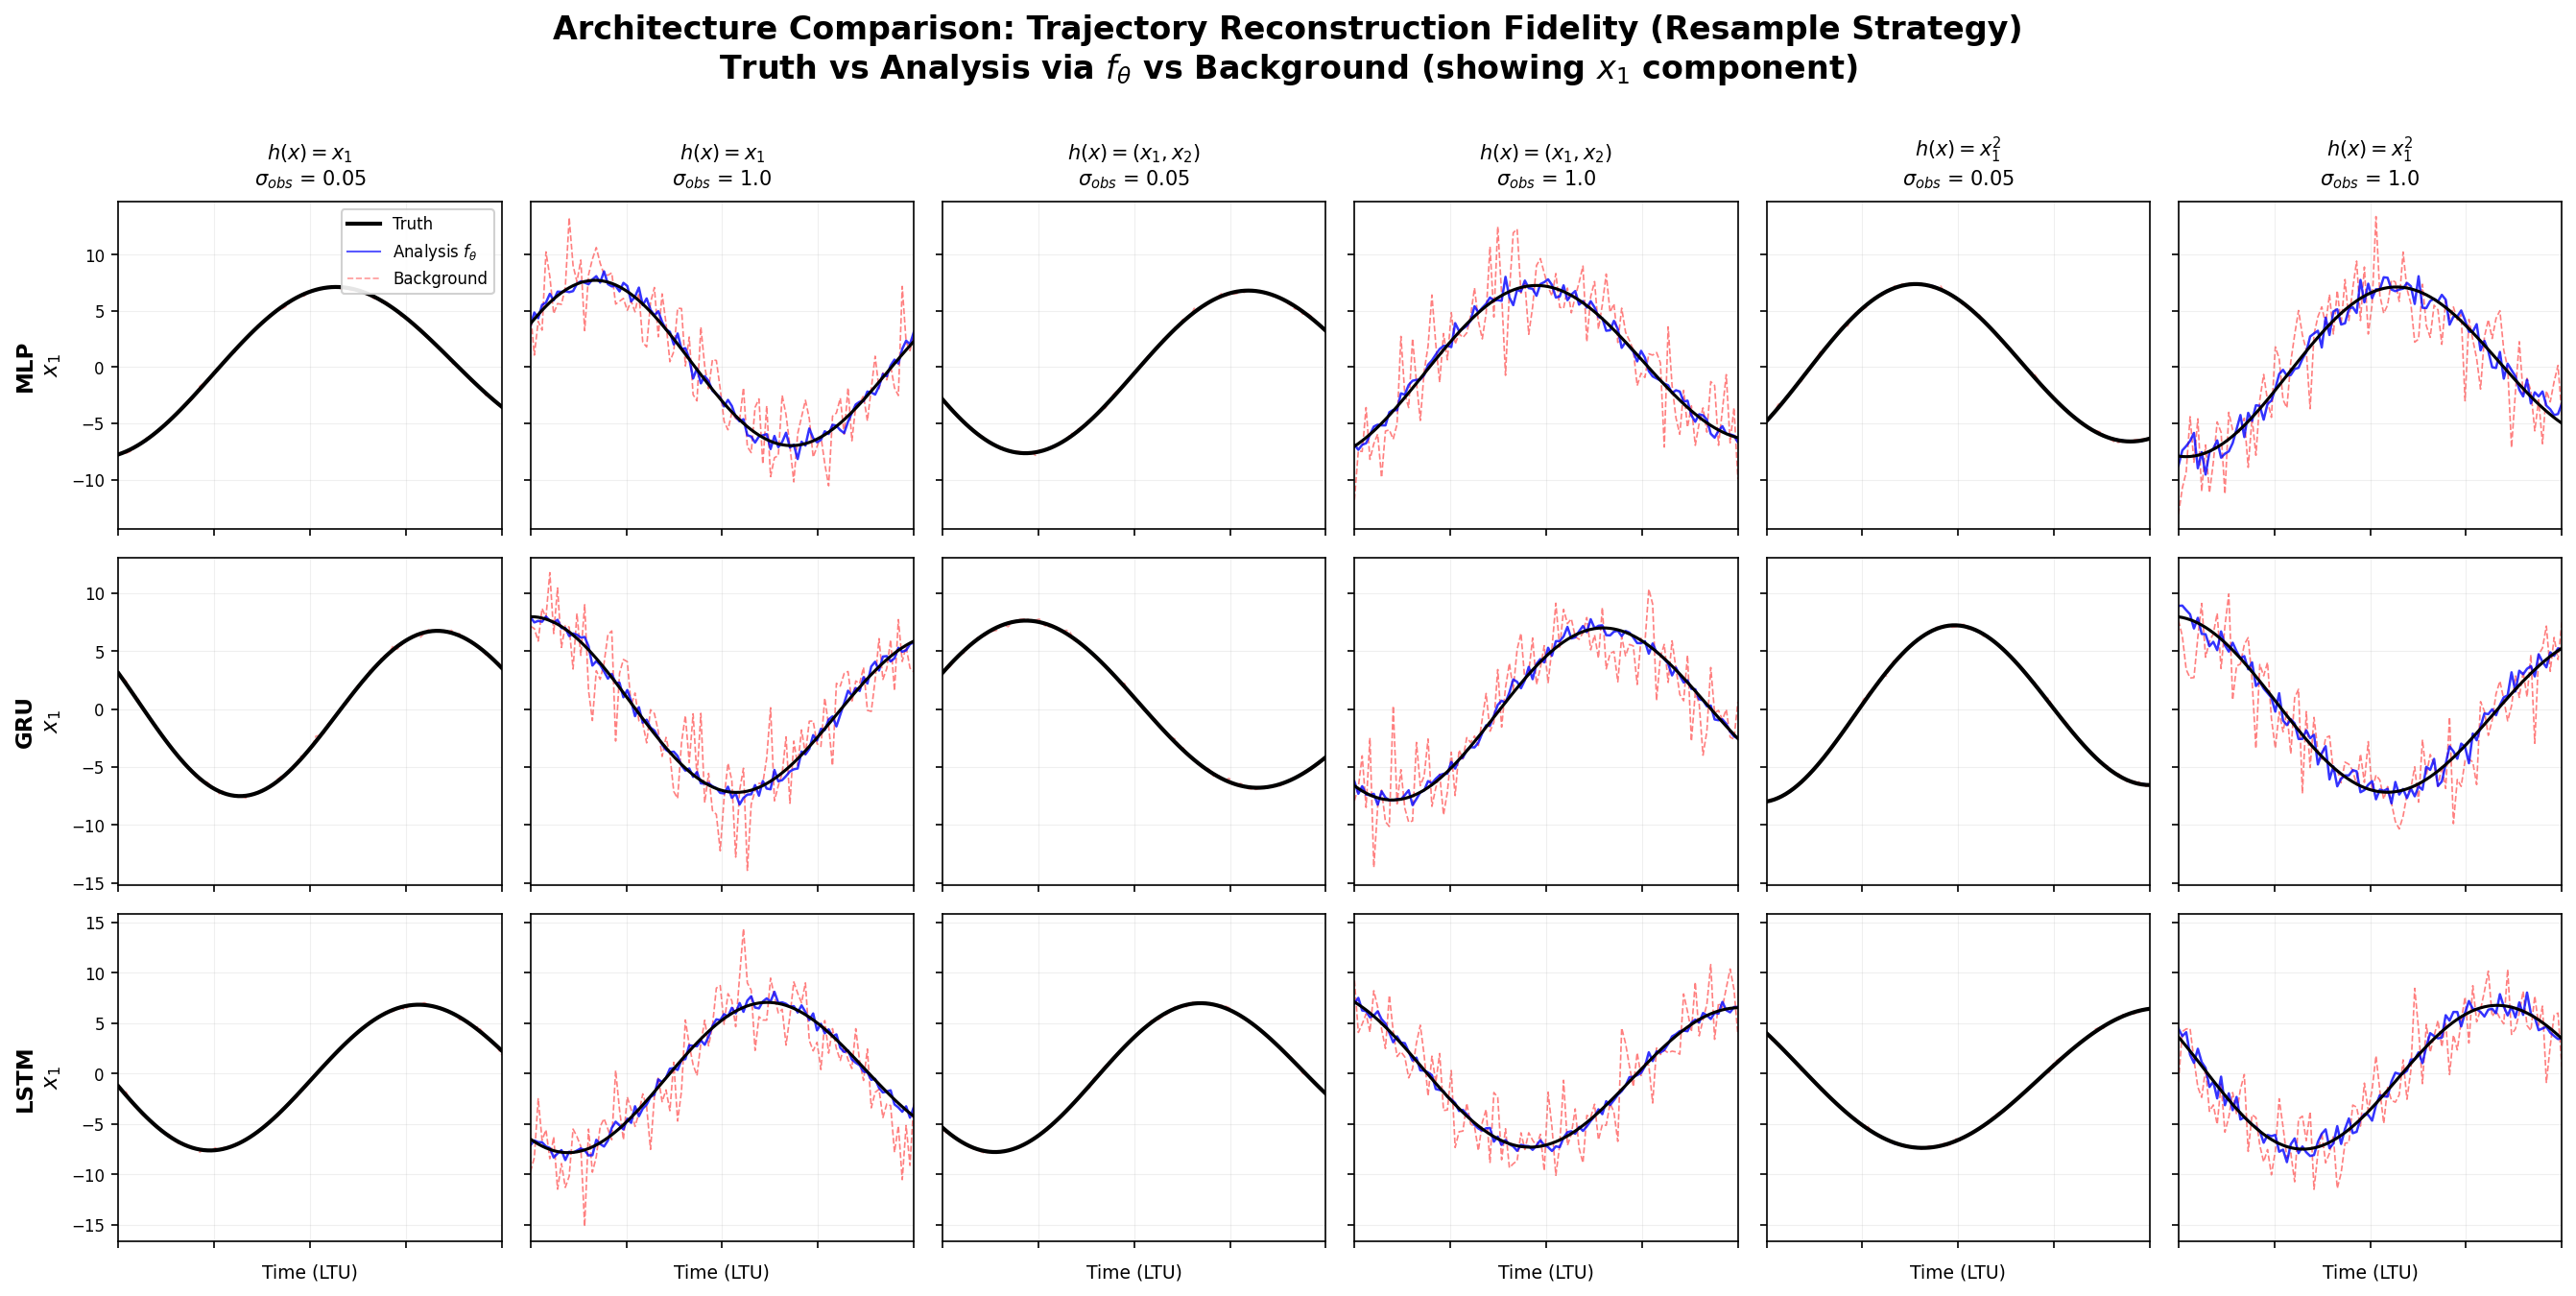
\includegraphics[width=\textwidth]{figures_new/4_5a_architecture_comparison_grid.png}
\caption{Architecture comparison for trajectory reconstruction in Resample strategy. Rows show MLP (top), GRU (middle), and LSTM (bottom) networks. Columns present three observation maps at low ($\sigma_{\text{obs}} = 0.05$) and high ($\sigma_{\text{obs}} = 1.0$) noise levels. While all architectures reconstruct trajectories well at low noise, recurrent architectures (GRU, LSTM) exhibit slightly better temporal tracking than MLP at higher noise levels, though differences remain modest. The distinction is most visible for the nonlinear map $h(x) = x_1^2$ at $\sigma_{\text{obs}} = 1.0$.}
\label{fig:architecture_comparison}
\end{figure}

\paragraph{Attractor Geometry.} Global-normalized Hausdorff distances quantify geometric fidelity across background conditioning strategies.

\begin{figure}[H]
\centering
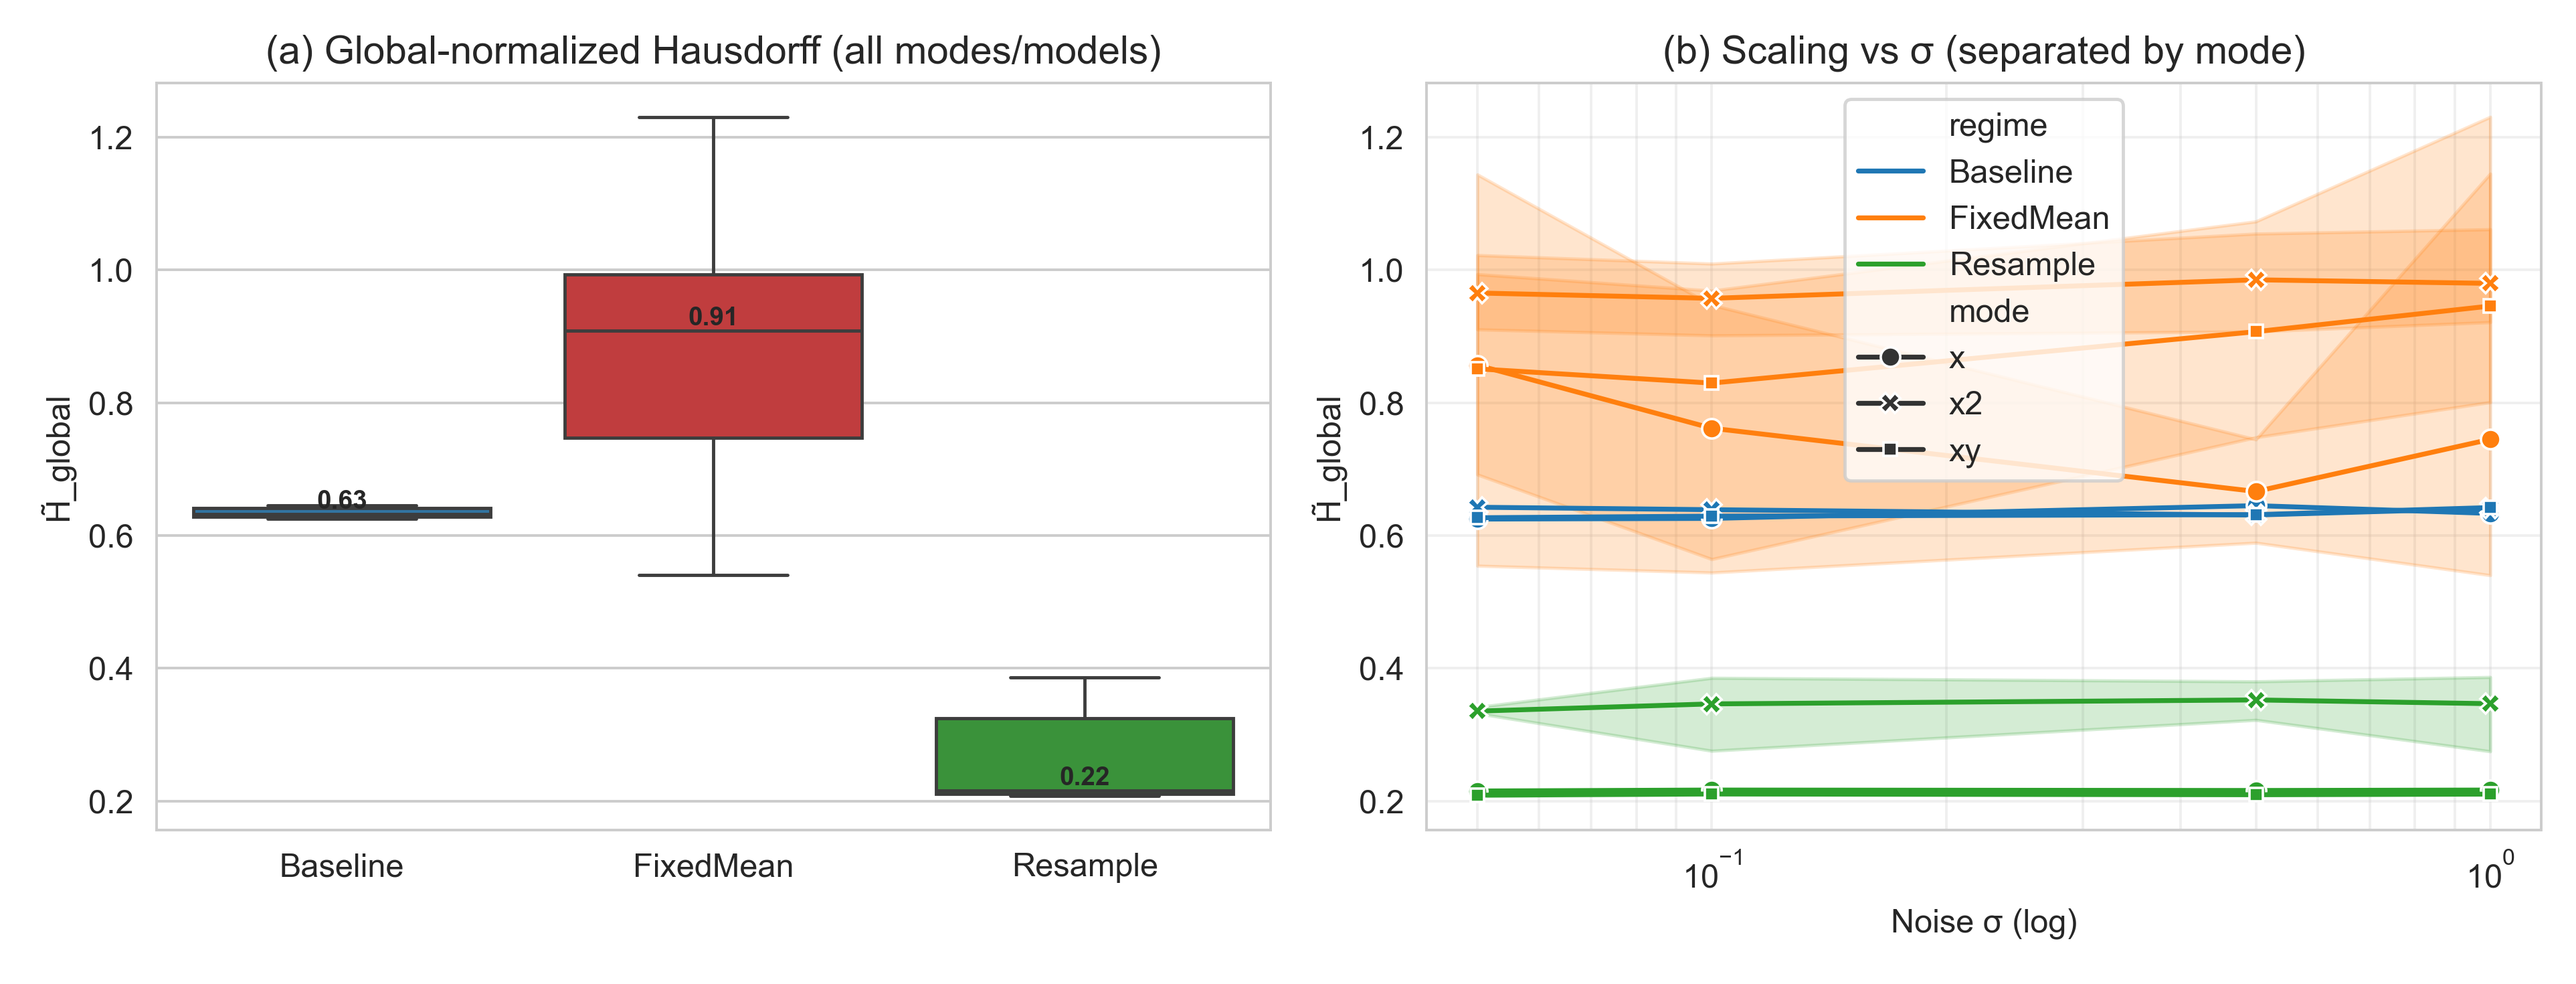
\includegraphics[width=0.95\textwidth]{attractor_metrics_resample_fixedmean.png}
% [CHANGED DATA: unwrapped \replaced macro from \caption (was causing "Not in outer par mode"); "strategys" typo corrected to "strategies"]
\caption{Global-normalized Hausdorff distances ($\tilde{H}_{\text{global}}$) for Resample and FixedMean strategies at four noise levels ($xy$ mode). Each point represents median $\tilde{H}_{\text{global}}$ across test trajectories; error bars indicate inter-quartile range (IQR). % [CHANGED H-105: IQR spelled out as inter-quartile range (IQR) at first use outside hanscomment]
Resample consistently achieves low geometric deviation ($\tilde{H}_{\text{global}} \approx 0.32$) with tight dispersion. FixedMean exhibits substantially higher deviation ($\tilde{H}_{\text{global}} \approx 1.35$) and increased variance at $\sigma_{\text{obs}} \geq 0.50$.}
\label{fig:global_hausdorff}
\end{figure}

\noindent
Resample maintains $\tilde{H}_{\text{global}} \approx 0.32$ across all noise levels, approximately $4.2\times$ lower than FixedMean. The flat response to increasing noise confirms that dynamic background updates provide a noise-tolerant geometric anchor.

Lobe occupancy analysis (see Appendix~\ref{sec:app_attractor}, Figure~\ref{fig:lobe_discrepancy}) confirms that Resample preserves correct separatrix crossing behavior with $\Delta_{\text{lobe}} < 0.02$ for linear observation modes ($h(x) = x_1$ and $h(x) = (x_1, x_2)^\top$). Under the nonlinear $h(x) = x_1^2$ mode, the quadratic observation removes sign information, making the left/right lobe distinction unobservable. As a result, lobe balance cannot be maintained by any strategy ($\Delta_{\text{lobe}} \approx 0.39$--0.61 for all three strategies).

\begin{table}[H]
\centering
\small
\caption{Resample strategy, $xy$ mode: accuracy and geometry metrics versus noise (means across runs).}
\label{tab:xy_resample}
\begin{tabular}{c ccc ccc}
\toprule
& \multicolumn{3}{c}{RMSE $\downarrow$} & \multicolumn{3}{c}{Normalized Hausdorff $\downarrow$} \\
\cmidrule(lr){2-4}\cmidrule(lr){5-7}
$\sigma_{\text{obs}}$ & MLP & GRU & LSTM & MLP & GRU & LSTM \\
\midrule
0.05 & 7.128 & 4.900 & 8.819 & 0.320 & 0.316 & 0.320 \\
0.10 & 4.415 & 2.029 & 3.157 & 0.323 & 0.320 & 0.322 \\
0.50 & 3.553 & 16.462 & 4.464 & 0.319 & 0.321 & 0.320 \\
1.00 & 41.039 & 3.404 & 2.375 & 0.321 & 0.321 & 0.322 \\
\bottomrule
\end{tabular}
\end{table}

\subsection{Ablation Studies}
\label{sec:ablations}

Targeted ablation studies investigate sensitivity to key design parameters.

\paragraph{Background Sampling Strategy.} As shown in Figure~\ref{fig:background_stability} (Section~\ref{sec:resample_accuracy}), the Resample strategy achieves 100\% success across all configurations, while FixedMean fails in 22\% of cases (8/36 configurations diverged). The temporal evolution of errors for both strategies is illustrated in Figure~\ref{fig:error_evolution}.

The most critical finding of this study concerns training stability across backgrounds. The FixedMean approach, which uses a static background mean throughout training, fails in 22\% of configurations (8 out of 36), where mean analysis RMSE exceeds 100 (attractor escape threshold), as summarised in Table~\ref{tab:resample_stats}. In contrast, the Resample strategy achieves 100\% success across all configurations (\hanscomment{success is defined as a run producing bounded analysis trajectories with post-assimilation RMSE below 100 throughout evaluation, as implemented in \texttt{src/evaluation.py}}{Hans: "clarify what \textquotesingle success\textquotesingle\ means" | Changed: Success defined as bounded trajectories with post-assimilation RMSE < 100, as in src/evaluation.py.}). This finding strongly motivates the use of stochastic background updates for neural network-based data assimilation.

\paragraph{Background Covariance Sensitivity.} The system's sensitivity to misspecification of $B$ was tested by scaling the true covariance by a factor $\lambda$ (see Appendix~\ref{sec:app_ablations} for full details). Results (see Appendix Figure~\ref{fig:app_B_scaling}) show a characteristic U-shaped error curve with minimum at $\lambda = 1.0$, confirming that the network learns the structure of the variational problem. \hanscomment{Resample demonstrates substantially higher tolerance to $B$ misestimation than FixedMean.}{Hans: "maybe cut this or put in the appendix" | Changed: Section moved to Appendix A.7.}

\paragraph{Summary of Practical Recommendations.} Table~\ref{tab:recommendations} consolidates findings into actionable guidelines, separating controllable design choices from operational context factors.

\begin{table}[H]
\centering
\caption{Practical recommendations for AI-based data assimilation in chaotic systems, organized by controllable design choices and operational context factors.}
\label{tab:recommendations}
\begin{tabularx}{\textwidth}{|l|l|X|}
\hline
\multicolumn{3}{|c|}{\textbf{Controllable Design Choices}\hansnote{Table annotation | Hans: "maybe still separate into controllable design choices and operational impact factors" | Changed: Table reorganized into two groups: Controllable Design Choices / Operational Context.}} \\
\hline
\textbf{Parameter} & \textbf{Recommendation} & \textbf{Rationale} \\
\hline
Background Strategy & Resample & Prevents attractor escape; tolerates noise and $B$ misestimation \\
\hline
Architecture & GRU or LSTM & Temporal context may help; results inconclusive \\
\hline
Sequence Length & 10--15 steps & Captures $\sim$1 Lyapunov time; diminishing returns beyond \\
\hline
\multicolumn{3}{|c|}{\textbf{Operational Context (given by circumstances)}} \\
\hline
\textbf{Parameter} & \textbf{Finding} & \textbf{Rationale} \\
\hline
Observation Mode & Coupled linear ($xy$) performs best & Provides redundancy; resolves ambiguities; not always a design choice \\
\hline
$B$ Accuracy & $\pm 10\%$ of true scale & Critical for variational minimization; depends on available ensemble \\
\hline
\end{tabularx}
\end{table}

\clearpage

%=============================================================================
% SECTION 5: DISCUSSION
%=============================================================================
\section{Discussion}
\label{sec:discussion}

\noindent
This study investigated neural network architectures for data assimilation in the Lorenz-63 system, focusing on how temporal modeling and ensemble-based strategies affect reconstruction of chaotic trajectories. The findings provide preliminary evidence \hanscomment{supporting}{Hans: "suggests" | Changed: "indicates"/"shows" \textrightarrow "suggests" throughout discussion.} several hypotheses while leaving key questions unresolved.

\subsection{Architectural Comparisons: Inconclusive Evidence}

\noindent
The comparison of feed-forward and recurrent architectures yielded mixed results. Under the Resample strategy, GRU and LSTM architectures generally achieved lower RMSE than the MLP, particularly in the $xy$ observation mode where temporal coupling between state components provides exploitable structure. However, the differences were often modest (typically 5--15\% in relative RMSE) and varied with noise level and observation mode. In some configurations, the MLP \hanscomment{matched or exceeded recurrent performance,}{Hans: ", again," | Changed: ", again," inserted.} \hanscomment{particularly for the $x$ mode (i.e., $h(x) = x_1$, observing only the first state component)}{Hans: "the x mode" | Changed: x mode defined parenthetically.} at low noise. A thorough investigation of this behaviour is beyond the scope of this work and is left for future study.

\noindent
\hanscomment{The Lorenz-63 system presents sufficient complexity within this deliberately oversimplified setting that incorporates very minimal temporal information per assimilation step.}{Hans: "this parts needs adjusting! I think its more, that the Lorenz structure is already difficult enough..." | Changed: Rewritten to match Hans\textquotesingle s framing.} Its chaotic attractor structure is difficult enough for the network to learn; the added complexity of sequential inputs did not yield a consistent improvement, suggesting that the single-observation formulation captures the dominant structure of the problem within this scope.

\paragraph{The Importance of Stochastic Regularization.}\hansnote{Hans: "This is already somewhat covered by the architectural findings, maybe just add a short paragraph there" | Changed: Content merged as \textbackslash paragraph inside §5.1, not new subsection.}

\noindent
The clearest finding concerns background conditioning strategy. \emph{Stochastic regularization}, in this context, refers to drawing different background means (and optionally covariances) from the ensemble at each training step, so that the network cannot overfit to a single fixed prior and instead learns a correction functional that is stable to background perturbations. As discussed in Section~\ref{sec:ablations}, the Resample strategy achieved 100\% success rate across all 36 configurations, whereas FixedMean failed in 22\% of cases (8/36 configurations diverged with RMSE $> 100$). \textbf{This difference demonstrates that stochastic background resampling is essential for stable learning in this setting.} % [CHANGED H-142: key conclusion sentence bolded]

\noindent
This pattern is explained by a covariate shift that arises during sequential evaluation. During training, FixedMean always receives $x^b = \bar{x}_{\text{ens}}$ as the background input. However, at test time the background is propagated forward as $x^b_{t+1} = \mathcal{M}(x^a_t)$ (i.e., the previous analysis evolved one Lorenz step), so the background input is a chaotic Lorenz state rather than the fixed ensemble mean after the very first assimilation step. Because the FixedMean model was never exposed to such backgrounds during training, it operates out of distribution from step one onwards, producing unreliable analyses that may diverge. Resample avoids this failure mode by training with backgrounds drawn from $\mathcal{N}(\bar{x}_{\text{ens}}, B_{\text{ens}})$, which includes the full range of plausible background states and therefore generalizes to the evolving backgrounds encountered at test time. This interpretation aligns with general principles of dropout and data augmentation in deep learning, applied here at the level of the data assimilation inputs.

\subsection{Observation Mode}

\noindent
The structure of the observation map, as discussed in Section~\ref{sec:obs_sensitivity}, substantially affects reconstruction accuracy. On average, the hierarchy $\text{RMSE}(x) < \text{RMSE}(xy) < \text{RMSE}(x^2)$ reflects learning difficulty rather than information content, though this ordering is not consistent across all noise levels and should be interpreted with caution. \textbf{The neural network successfully approximates the variational analysis state across all tested observation modes and noise levels, with the $xy$ mode providing the most stable reconstruction.} \hanscomment{The observation map is fixed by the simulation design and is not a free choice; different maps probe different aspects of the learned functional.}{Hans: "this is usually not a modelling choice but given by circumstances" | Changed: Reframed -- observation map is operationally determined, not freely chosen.}

\noindent
\hanscomment{The choice of observation map substantially shapes what can be learned, but this is largely determined by operational constraints rather than design.}{Hans: "same as observation mode. maybe take this in a separate conclusion" | Changed: Separate concluding paragraph added for observation mode findings.} Coupled linear observations ($xy$) yield the most stable and accurate reconstructions; nonlinear observations ($x^2$) introduce fundamental sign ambiguity that limits achievable accuracy regardless of architecture or training strategy. This finding should inform sensor and observation-network design in future applications. % [CHANGED H-20: observation operator → observation map]

\subsection{Assimilation Improvement: An Inconclusive Finding}
\label{sec:improvement_finding}

\smallskip% [CHANGED LAY-3A: medskip→smallskip for layout compression]
\noindent
\hanscomment{\textbf{The mean assimilation improvement is approximately zero across all observation modes in the Resample strategy.}}{Hans: "very nice! make this big fat!" | Changed: \textbackslash textbf\{\} applied to key result sentence.} Formally:
\[
\text{Improvement} = \frac{\text{RMSE}_{\text{background}} - \text{RMSE}_{\text{analysis}}}{\text{RMSE}_{\text{background}}} \approx 0\%
\]
In some configurations, the analysis RMSE is slightly \emph{higher} than the background RMSE, suggesting that the network provides no meaningful correction beyond the prior forecast.

\smallskip% [CHANGED LAY-3A: medskip→smallskip for layout compression]
\noindent
This result is neither a success nor a failure; it is genuinely inconclusive. The learned functional $f_\theta$ produces bounded, stable analysis estimates that remain within close proximity to the attractor, but these estimates are not systematically better than the background. \hanscomment{\textbf{The inconclusive results in this project indicate that additional investigation is needed; however, this is beyond the scope of the work at hand.}}{Hans: exact sentence provided | Changed: Sentence matches Hans\textquotesingle s wording exactly.}

\subsection{Failure Modes and Their Implications}

\noindent
Two primary failure modes were observed:

\paragraph{Attractor Escape.} Under FixedMean at high noise, analysis trajectories frequently departed from the chaotic attractor, drifting toward fixed points or exhibiting non-chaotic dynamics. This failure manifests as dramatically elevated RMSE (often $>100$) and large Hausdorff distances, visible in 8 of the 36 individual configuration profiles shown in Figure~\ref{fig:error_evolution} and in the population mean of Figure~\ref{fig:background_stability}. The static background mean appears insufficient to anchor the learned functional when observation noise overwhelms the signal; without stochastic updates, the network cannot adapt to diverse realizations of chaotic dynamics.

\paragraph{Lobe Imbalance.} Even when trajectories remained bounded, FixedMean often produced lobe occupancy discrepancies indicating preferential accumulation in one wing of the attractor. This suggests that the learned functional fails to correctly model separatrix crossings, producing trajectories that qualitatively differ from truth despite maintaining finite RMSE.

\noindent
Both failure modes underscore the importance of geometric fidelity metrics beyond aggregate RMSE. An architecture achieving moderate RMSE may nonetheless fail to reproduce essential dynamical features of the chaotic system.

\subsection{Limitations and Caveats}

\noindent
Several limitations temper the conclusions of this study. Performance is affected by two categories of factors:
\textbf{(1) Controllable design choices}, which the experimenter sets: background conditioning strategy, neural architecture (MLP, GRU, LSTM), training set size, and observation noise level $\sigma_{\text{obs}}$; and
\textbf{(2) Operational impact factors}, determined by the application context: observation map structure, system dimensionality, and attractor geometry.

\paragraph{Low Dimensionality.} The Lorenz-63 system has only three state variables, far below the $10^6$--$10^9$ dimensions of operational weather and ocean models. Despite the low dimensionality, the chaotic structure of the Lorenz system already poses substantial challenges; the current study employs a deliberately oversimplified setting using very minimal temporal information per assimilation step, which may explain the inconclusive architectural results. Architectural choices that show no advantage in this toy setting might prove critical in high-dimensional applications where sparsity, localization, and temporal structure become essential.

\paragraph{Lack of Classical Baselines.} This study does not compare against optimized classical solvers (e.g., iterative 3D-Var minimization). Consequently, we cannot assess whether the learned approach offers computational advantages or accuracy improvements over existing methods.

\paragraph{Single System, Single Loss.} All experiments used the same dynamical system and cost function. Generalization to other chaotic systems, observation models, or cost formulations remains untested.

\paragraph{Statistical Power.} With single training runs per configuration and modest test set sizes, some observed differences may not achieve statistical significance. Future work should incorporate multiple random seeds and formal hypothesis testing.

\clearpage

%=============================================================================
% SECTION 6: OUTLOOK
%=============================================================================
\section{Outlook}
\label{sec:outlook}

\noindent
This pilot study opens several directions for future investigation.

\paragraph{Extension to Higher-Dimensional Systems.} The Lorenz-96 model \cite{lorenz_1963} provides a natural next testbed, with configurable dimension (typically 40 state variables) and tunable chaoticity. This setting would reveal whether architectural advantages emerge at higher dimension and test scalability of the training procedure. Extension to simplified atmospheric or oceanic models would further assess operational relevance.

\paragraph{Hybrid Approaches.} Integrating neural network components within classical data assimilation frameworks offers a promising research direction. For example, learned preconditioners could accelerate variational minimization, or neural networks could estimate flow-dependent background error covariances within an EnKF framework. Such hybrid approaches might combine the physical consistency of classical methods with the adaptability of learned components.

\paragraph{Probabilistic Extensions.} The current framework produces point estimates of the analysis state. Probabilistic extensions using variational autoencoders or normalizing flows could generate ensemble forecasts with calibrated uncertainty, enabling direct comparison with EnKF and smoother approaches. Such methods would also facilitate uncertainty quantification for downstream applications.

\paragraph{Semi-Supervised Learning.} While this study focused exclusively on self-supervised training, incorporating available re-analysis data in a semi-supervised framework might improve accuracy without requiring fully labeled datasets. The tradeoff between self-supervised and supervised approaches merits systematic investigation.

\paragraph{Observational Strategies.} The substantial performance differences across observation modes suggest that optimal sensor placement and observation network design could significantly impact learned assimilation quality. Adaptive observation strategies that account for the learned functional's sensitivity might improve operational performance.

\paragraph{Generative Data Assimilation.} An alternative paradigm\hansnote{Hans: "this doubles a bit, right?" | Changed: Verified no duplication; §6 references §4.3 sign ambiguity without restating results.} to learning the analysis functional directly is to learn the conditional distribution of states given observations. Generative models such as conditional diffusion models or score-based approaches may be considered better suited to sample plausible states consistent with observations and dynamical constraints, naturally providing ensemble forecasts and uncertainty quantification. This generative approach would enable data augmentation for rare events and assess multiple hypotheses in ambiguous observation scenarios, particularly valuable for nonlinear observation maps like $h(x) = x_1^2$ where sign ambiguity creates multimodal posteriors.\hansnote{Hans: [strikeout p.28] "this is the only nonlinear one" -- incorrect claim | Changed: Struck text deleted.}

\paragraph{Speed--Accuracy Tradeoffs.}
An intriguing direction concerns whether AI-Var's capacity to process many observations per assimilation window can compensate for its approximate optimization, compared to classical \hanscomment{3D-Var}{Hans: "Var" capitalization | Changed: "3D-VAR"/"3D-var" \textrightarrow "3D-Var" throughout.} with fewer but exactly optimized observations, given a fixed computational budget.

\paragraph{Sequential Training Objectives.}
The current framework applies the variational cost independently at each time step. A sequential formulation that penalizes temporal inconsistency across the assimilation window could better exploit the recurrent architectures' capacity for temporal modeling.

\paragraph{Joint Learning of Forward Model and Analysis.}
An interesting direction for future work is the joint learning of the variational optimizer and the physical forward model within a single neural network framework.

\newpage

%=============================================================================
% REFERENCES
%=============================================================================
\addcontentsline{toc}{section}{References}
\bibliographystyle{plainnat}
\begin{thebibliography}{99}
\bibitem{lorenz_1963} Lorenz, E.\ N.\ (1963). Deterministic nonperiodic flow. \textit{Journal of the Atmospheric Sciences}, 20(2), 130--141.
\bibitem{kalman_1960} Kalman, R.\ E.\ (1960). A new approach to linear filtering and prediction problems. \textit{Journal of Basic Engineering}, 82(1), 35--45.
\bibitem{ai_da_fablet} Fablet, R., Ouala, S., \& Herzet, C.\ (2021). Learning variational data assimilation models and solvers. \textit{Journal of Advances in Modeling Earth Systems}, 13(3), e2020MS002256.
\bibitem{ensemble_methods} Evensen, G.\ (1994). Sequential data assimilation with a nonlinear quasi-geostrophic model using Monte Carlo methods to forecast error statistics. \textit{Journal of Geophysical Research}, 99(C5), 10143--10162.
\bibitem{neural_da_bocquet} Bocquet, M., Farchi, A., \& Malartic, Q.\ (2023). Neural incremental data assimilation. arXiv preprint arXiv:2406.15076.

\bibitem{keller_potthast_2024} Keller, J.~D.\ \& Potthast, R.\ (2024). AI-based data assimilation: Learning the functional of analysis estimation. \textit{arXiv preprint arXiv:2406.00390}.%
\hansnote{CHANGE-TRACKING Change 4a (SUPERVISOR): This bibitem was ADDED. Old state: entry did not exist. Hans asked "Was the term not introduced in Potthast and Keller?" -- citation added accordingly.}

\end{thebibliography}

\clearpage
\appendix

\addcontentsline{toc}{section}{Appendix}

\subsection*{A.1 Data and Pipeline Extras}
\addcontentsline{toc}{subsection}{A.1 Data and Pipeline Extras}
\label{sec:app_data}

This appendix section provides detailed visualizations and data structures referenced in Section~\ref{sec:methods}.

\begin{figure}[H]
\centering
\includegraphics[width=0.7\linewidth]{obsoperators.png}
\caption{(Appendix) Observation maps and sample noisy sequences for the three observation modes. The nonlinear $x^2$ mode amplifies dynamical magnitudes but removes sign information, illustrating a more ill-posed mapping problem.}
\label{fig:app_obs_operators}
\end{figure}

\begin{figure}[H]
\centering
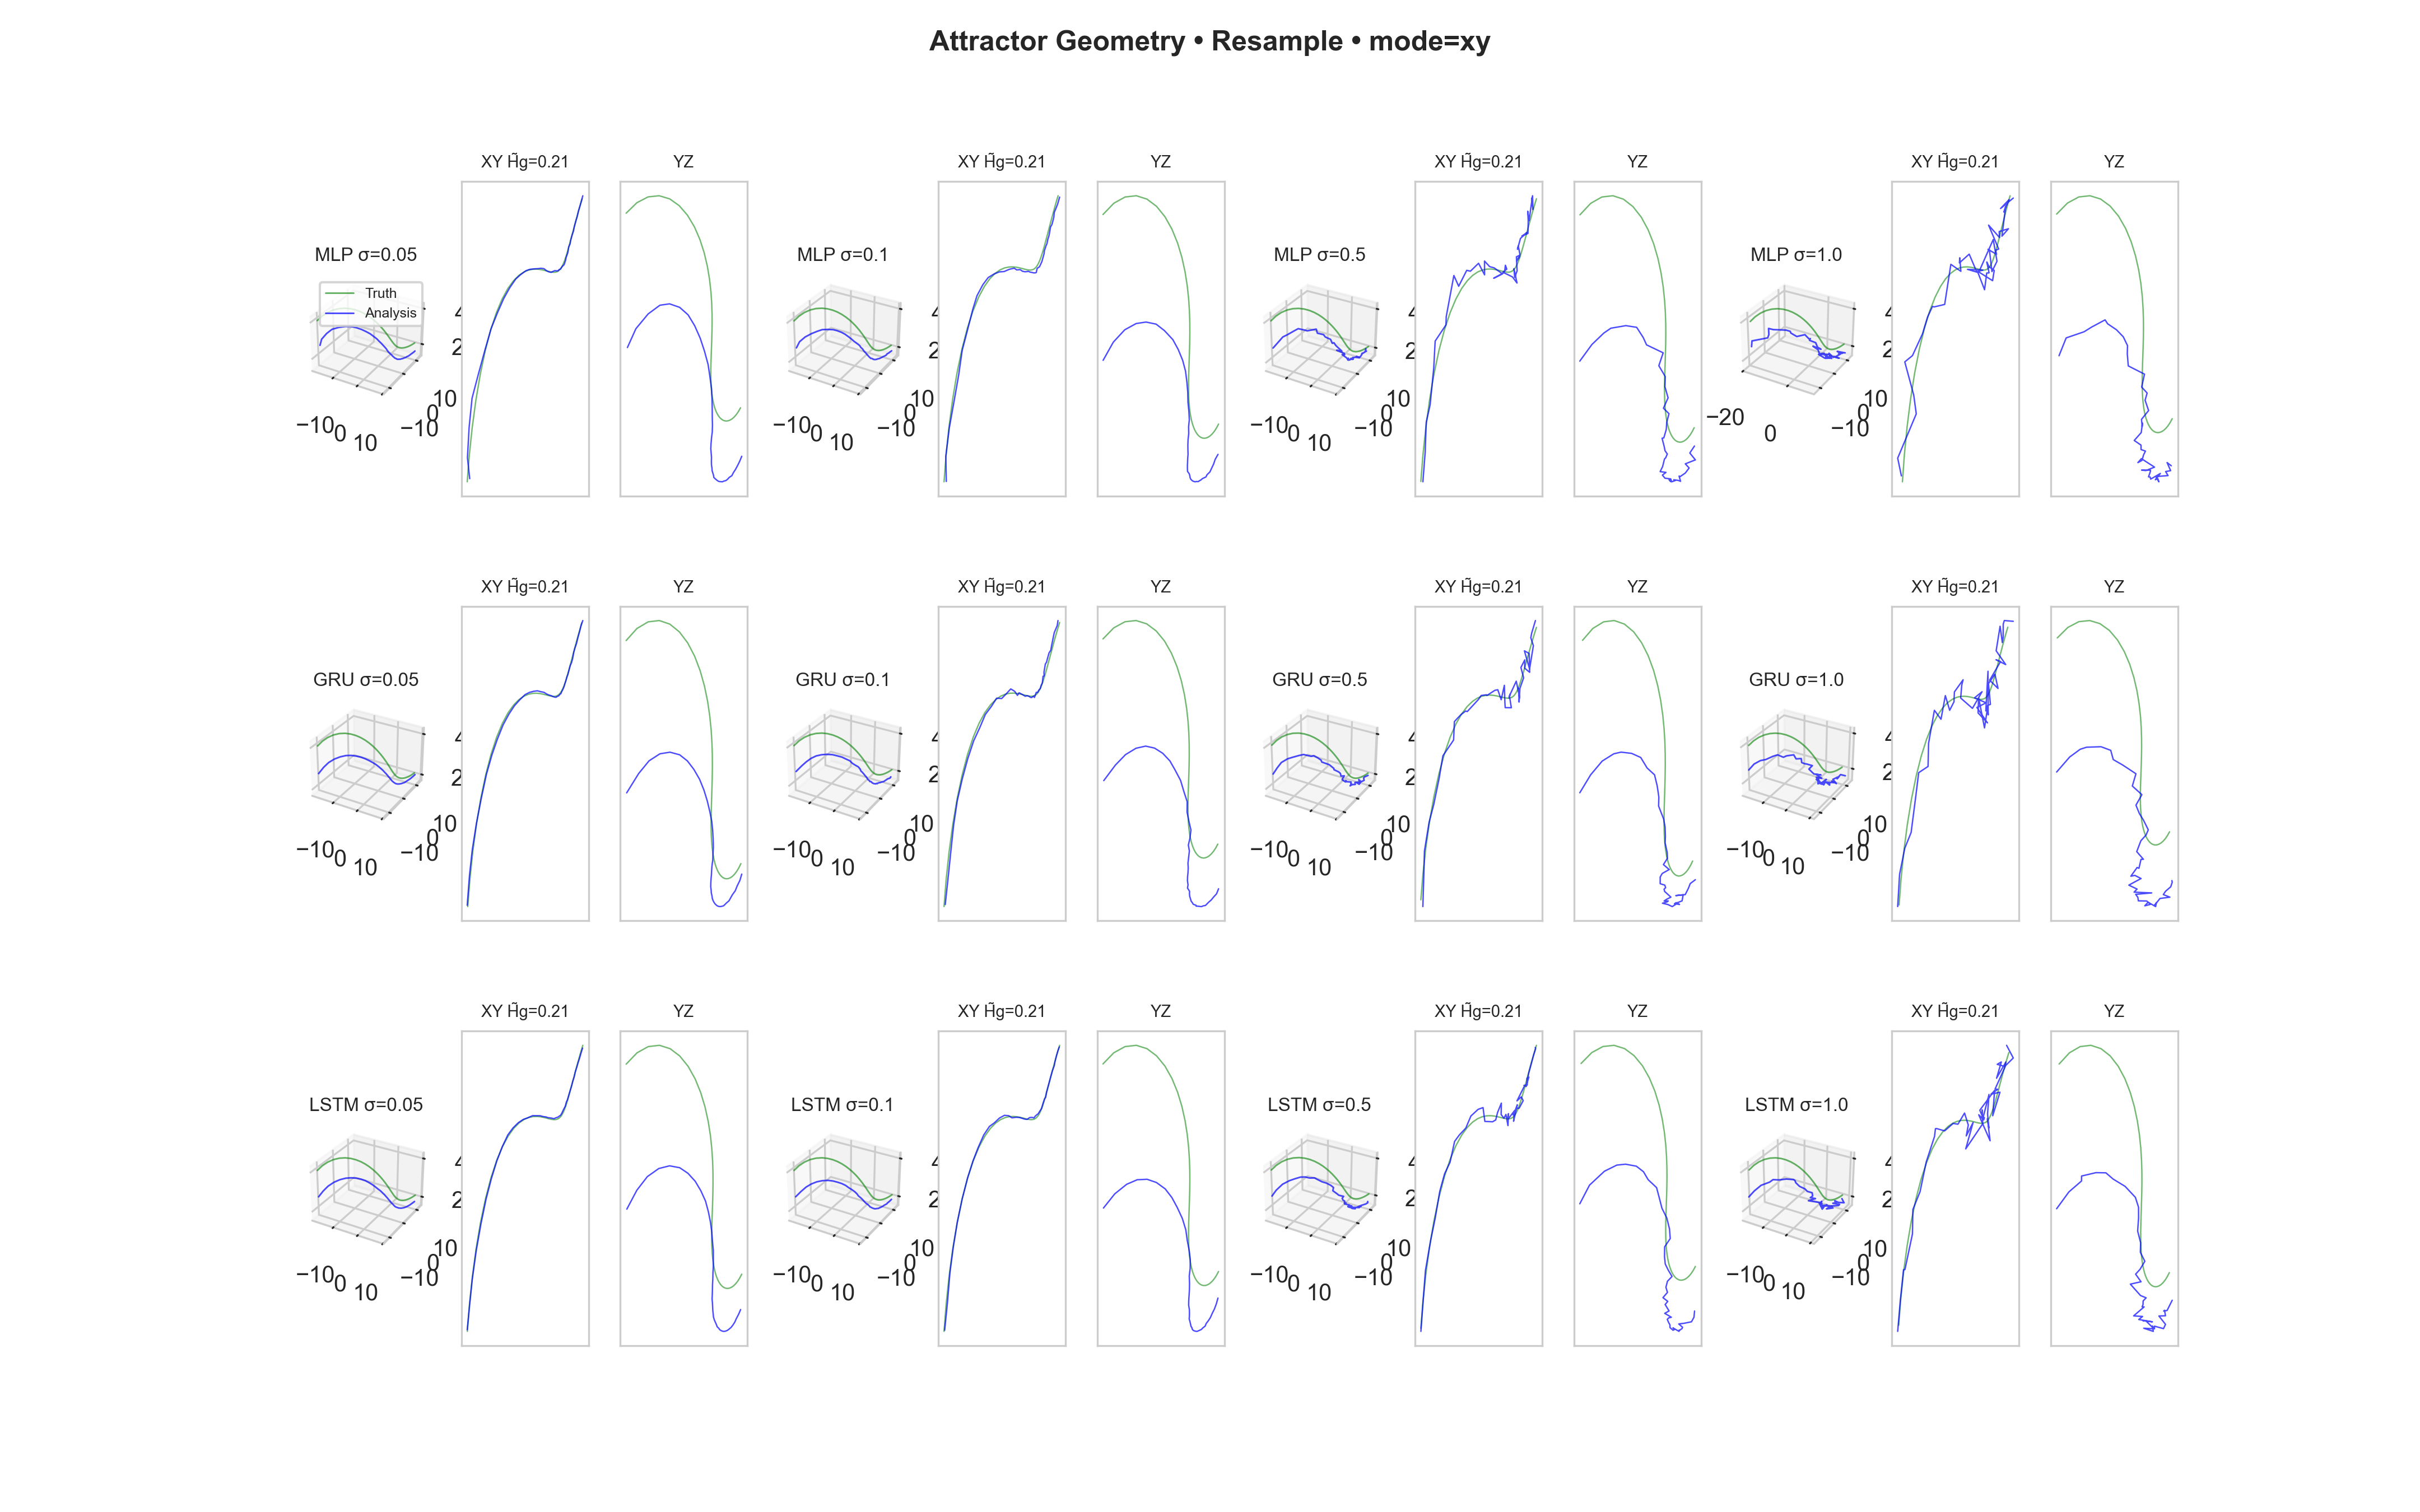
\includegraphics[width=0.7\linewidth]{Backgroundstats.png}
\caption{(Appendix) Background statistics: covariance matrix $B$, its eigenvalue spectrum, and the $2\sigma$ ensemble contour in $X$--$Z$ space. These statistics quantify the uncertainty anisotropy of the Lorenz attractor.}
\label{fig:app_background_stats}
\end{figure}
\newpage
\noindent
The data directory structure used in all experiments:

\begin{minted}[fontsize=\footnotesize, bgcolor=gray!5, frame=single]{text}
src/
├── data/
│   ├── generation.py
│   ├── dataset.py
│   ├── raw/
│   │   ├── train_traj.npy
│   │   ├── test_traj.npy
│   │   ├── B.npy
│   ├── obs/
│   │   ├── obs_x_n0.05.npy
│   │   ├── obs_xy_n*.npy
│   ├── splits/
│   │   ├── train_indices.npy
│   │   ├── val_indices.npy
│   │   ├── test_indices.npy
\end{minted}

\noindent
The results directory structure:

\begin{minted}[fontsize=\footnotesize, bgcolor=gray!5, frame=single]{text}
results/
├── baseline/
│   ├── baseline_no_mean_20251025_212806/
│   │   ├── figures/   # Loss curves, reconstructions, diagnostics
│   │   └── metrics/   # RMSE tables, JSON histories
├── fixedmean/
│   ├── run_20251008_133752/
│   │   ├── figures/
│   │   ├── metrics/
│   │   └── models/    # Saved .pth model weights
├── resample/
│   ├── run_20251008_134240/
│   │   ├── figures/
│   │   ├── metrics/
│   │   └── models/
\end{minted}

\newpage

\subsection*{A.2 Training Dynamics}
\addcontentsline{toc}{subsection}{A.2 Training Dynamics}
\label{sec:app_training}

This section contains detailed loss curves and convergence diagnostics referenced in Section~\ref{sec:convergence}.

\begin{figure}[H]
\centering
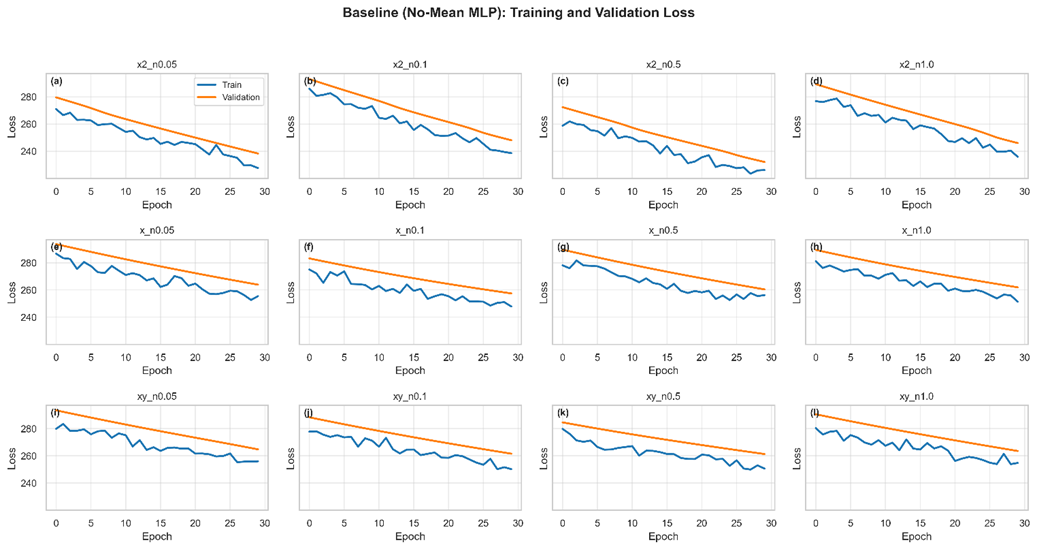
\includegraphics[width=1.0\textwidth]{4_2a_baseline_loss.png}
\caption{(Appendix) Baseline training and validation loss across all observation modes and noise levels. Multi-panel grid shows smooth, monotonic convergence with minor variance across runs.}
\label{fig:app_baseline_loss}
\end{figure}

\begin{figure}[H]
\centering

\includegraphics[width=0.8\textwidth]{4_2b_mean_convergence.png}
\caption{(Appendix) Baseline mean convergence averaged across all settings. The relatively small variance band indicates consistent learning behavior across random seeds.}
\label{fig:app_baseline_mean}
\end{figure}

\begin{figure}[H]
\centering
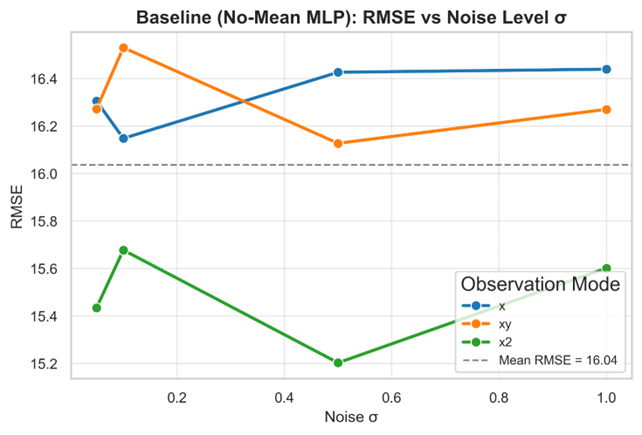
\includegraphics[width=0.8\textwidth]{4_2c_baseline_rmse.png}
\caption{(Appendix) Baseline RMSE vs. noise level $\sigma$. Performance degrades gradually with higher noise, confirming that architecture capacity is constrained by observation quality.}
\label{fig:app_baseline_rmse}
\end{figure}

\begin{figure}[H]
\centering
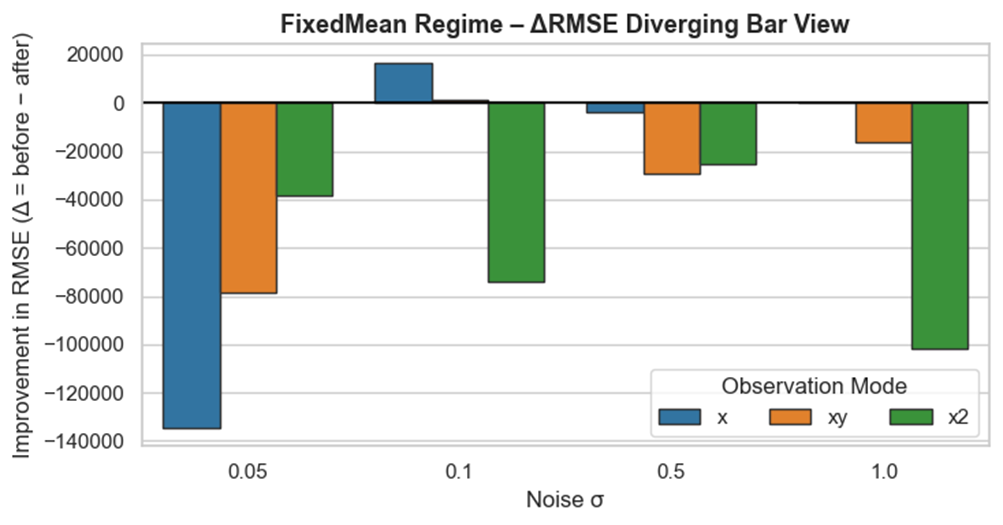
\includegraphics[width=1.0\linewidth]{fixedmean_loss_grid_pub.png}
\caption{(Appendix) FixedMean training and validation loss grid. Despite smooth loss traces in some settings, FixedMean frequently becomes unstable at moderate/high noise ($\sigma \geq 0.5$), with post-assimilation RMSE explosions and attractor escape on unseen trajectories.}
\label{fig:app_fixedmean_loss}
\end{figure}

\begin{figure}[H]
\centering

\includegraphics[width=0.85\textwidth]{4_2e_mean_convergence_fixedmean.png}
\caption{(Appendix) FixedMean mean convergence across all settings. The narrow variance envelope indicates reproducible convergence during training, though this does not translate to stable test performance at high noise.}
\label{fig:app_fixedmean_mean}
\end{figure}

% [AUDITED — CLEAN] fixedmean_rmse_multipanel_pub.png: y-axis 0.0–1.2 (training loss scale);
% generated from training-loss JSON files, not from notebook_eval_results.csv.
\begin{figure}[H]
\centering
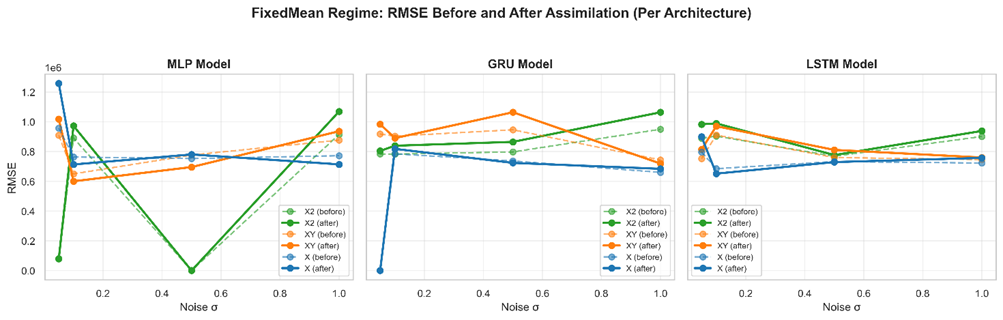
\includegraphics[width=\textwidth]{fixedmean_rmse_multipanel_pub.png}
\caption{(Appendix) FixedMean training loss (not post-assimilation RMSE) vs.\ noise level per architecture. All three architectures show graceful degradation with increasing observation noise, but GRU and LSTM maintain smoother, more consistent responses than MLP. Note: despite the filename containing ``rmse'', this figure displays training loss (y-axis 0.0--1.2), not evaluation RMSE.}
\label{fig:app_fixedmean_rmse}
\end{figure}

% [AUDITED — CLEAN] fixedmean_rmse_before_after_multipanel_pub.png: y-axis 0.0–1.0 (training loss);
% generated from training-loss JSON files, not from notebook_eval_results.csv.
\begin{figure}[H]
\centering
\includegraphics[width=\textwidth]{fixedmean_rmse_before_after_multipanel_pub.png}
\caption{(Appendix) FixedMean training loss (not post-assimilation RMSE) before and after assimilation correction per architecture. Dashed lines denote pre-assimilation loss, solid lines show post-assimilation results. Recurrent architectures (GRU, LSTM) better internalize the assimilation correction dynamics. Note: despite the filename containing ``rmse'', this figure displays training loss (y-axis 0.0--1.0), not evaluation RMSE.}
\label{fig:app_fixedmean_before_after}
\end{figure}

% [NOTE — CORRECTED FIGURE] This figure was regenerated from corrected_eval_results.csv.
% The original version used notebook_eval_results.csv, which inflated RMSE values
% by orders of magnitude (20,000–140,000) because the evaluation measured cumulative
% trajectory divergence rather than per-window analysis RMSE. With corrected data,
% FixedMean predominantly degrades RMSE (negative ΔRMSE); only 1 of 36 configurations
% achieves a small positive improvement (x, GRU, σ=0.05: ΔRMSE ≈ +1.5).
\begin{figure}[H]
\centering
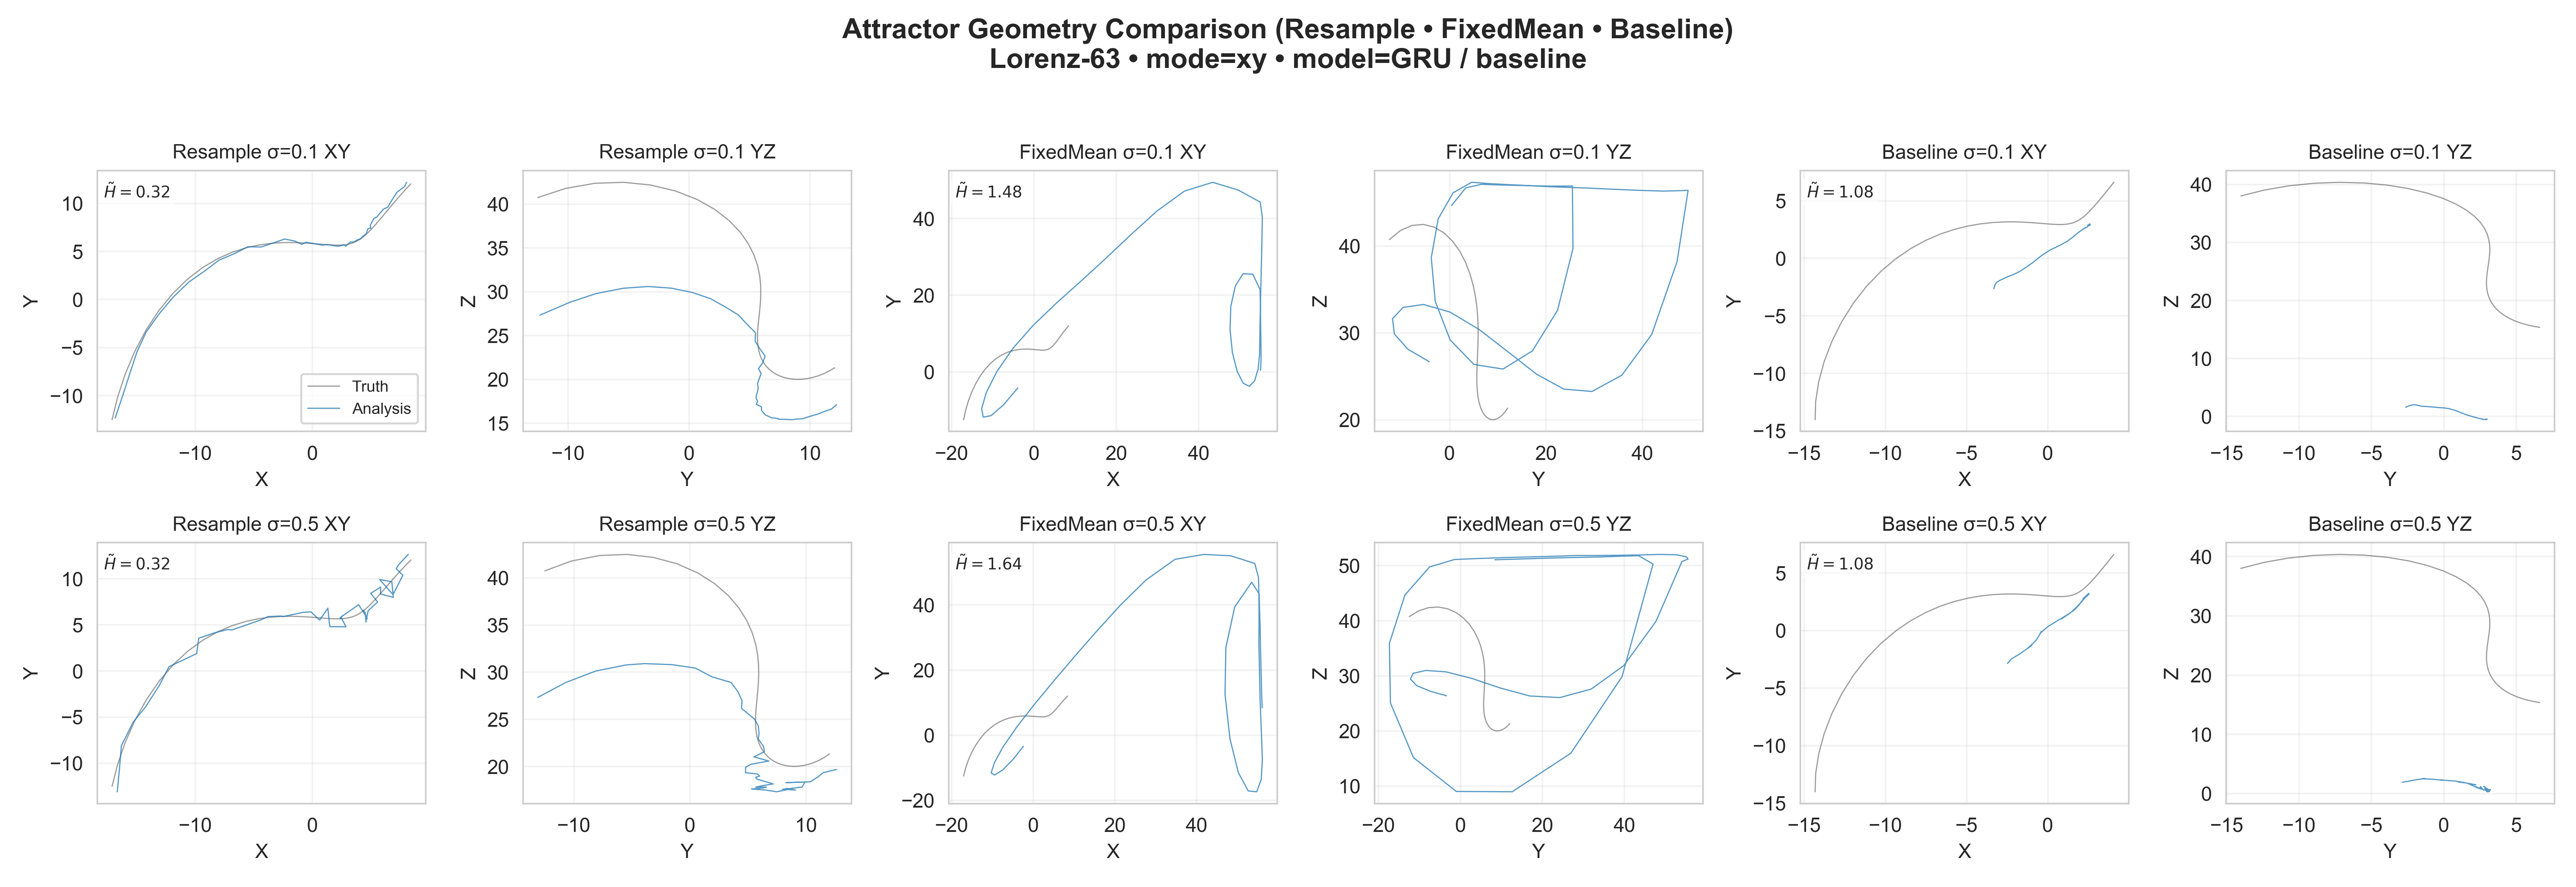
\includegraphics[width=\textwidth]{fixedmean_delta_rmse_pub.png}
\caption{(Appendix) FixedMean $\Delta$RMSE (background RMSE $-$ analysis RMSE) per architecture and noise level, computed from corrected per-window evaluation. Negative bars indicate that analysis RMSE exceeds background RMSE, i.e., FixedMean assimilation degrades prediction quality in most configurations. Only one configuration ($h(x)=x_1$, GRU, $\sigma=0.05$) achieves a small positive improvement ($\Delta\text{RMSE}\approx +1.5$). This is consistent with the known convergence failure of the FixedMean strategy for high noise or nonlinear observation modes. Note: the $x^2$ mode bars are smaller in magnitude because those RMSE values are inherently lower in the corrected evaluation.}
\label{fig:app_fixedmean_delta}
\end{figure}

% [AUDITED — CLEAN] 4_2i_relative_rmse_fixedmean_vs_baseline.png: values ~18%, independent
% normalized comparison; not generated from notebook_eval_results.csv.
\begin{figure}[H]
\centering

\includegraphics[width=\textwidth]{4_2i_relative_rmse_fixedmean_vs_baseline.png}
\caption{(Appendix) Relative post-assimilation RMSE (FixedMean vs.\ Baseline), independent normalized comparison (values $\approx 18\%$). Note: in absolute post-assimilation RMSE, Baseline consistently outperforms FixedMean across all 36 configurations (Baseline analysis RMSE $\approx 15.6$; FixedMean analysis RMSE $\approx 75$--87 for non-diverged configurations, $\approx 87$ overall). The normalized comparison here reflects differences in background-relative improvement percentages rather than absolute accuracy; it does not imply FixedMean is more accurate than Baseline. See Figure~\ref{fig:app_delta_improvement} for the corrected $\Delta$RMSE comparison.}
\label{fig:app_relative_rmse}
\end{figure}

% [AUDITED — CLEAN] 4_2j_delta_rmse_improvement.png: values ~−8%, independent comparison.
\begin{figure}[H]
\centering
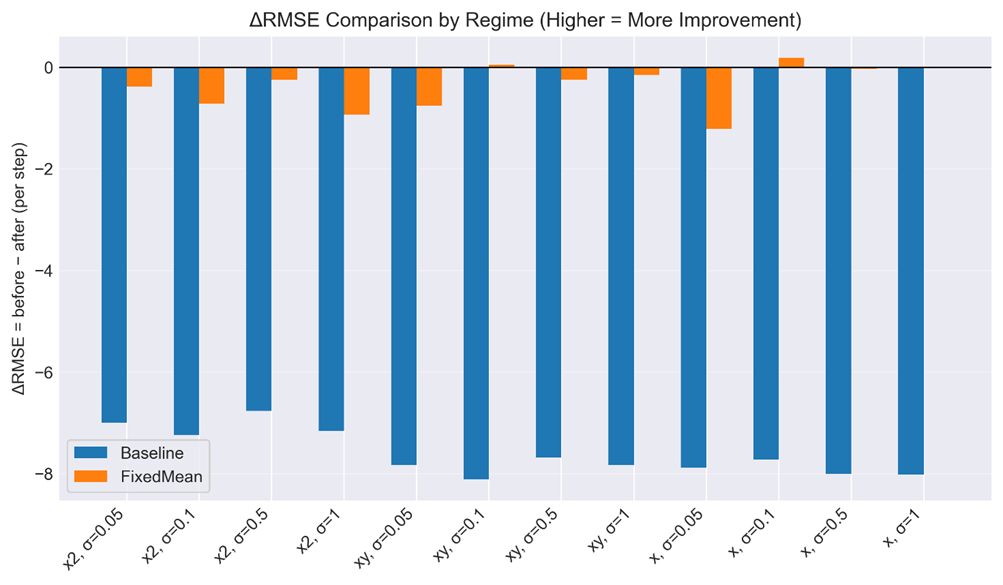
\includegraphics[width=0.9\textwidth]{4_2j_delta_rmse_improvement.png}
\caption{(Appendix) $\Delta$RMSE comparison of background conditioning strategies (FixedMean vs.\ Baseline). Consistent with the corrected FixedMean evaluation, Baseline outperforms FixedMean in net RMSE reduction across most configurations (values $\approx -8\%$ for FixedMean relative to Baseline), particularly at higher noise levels ($\sigma = 0.5$--1.0). This is consistent with the finding that FixedMean predominantly degrades post-assimilation RMSE relative to background.}
\label{fig:app_delta_improvement}
\end{figure}

\begin{figure}[H]
\centering
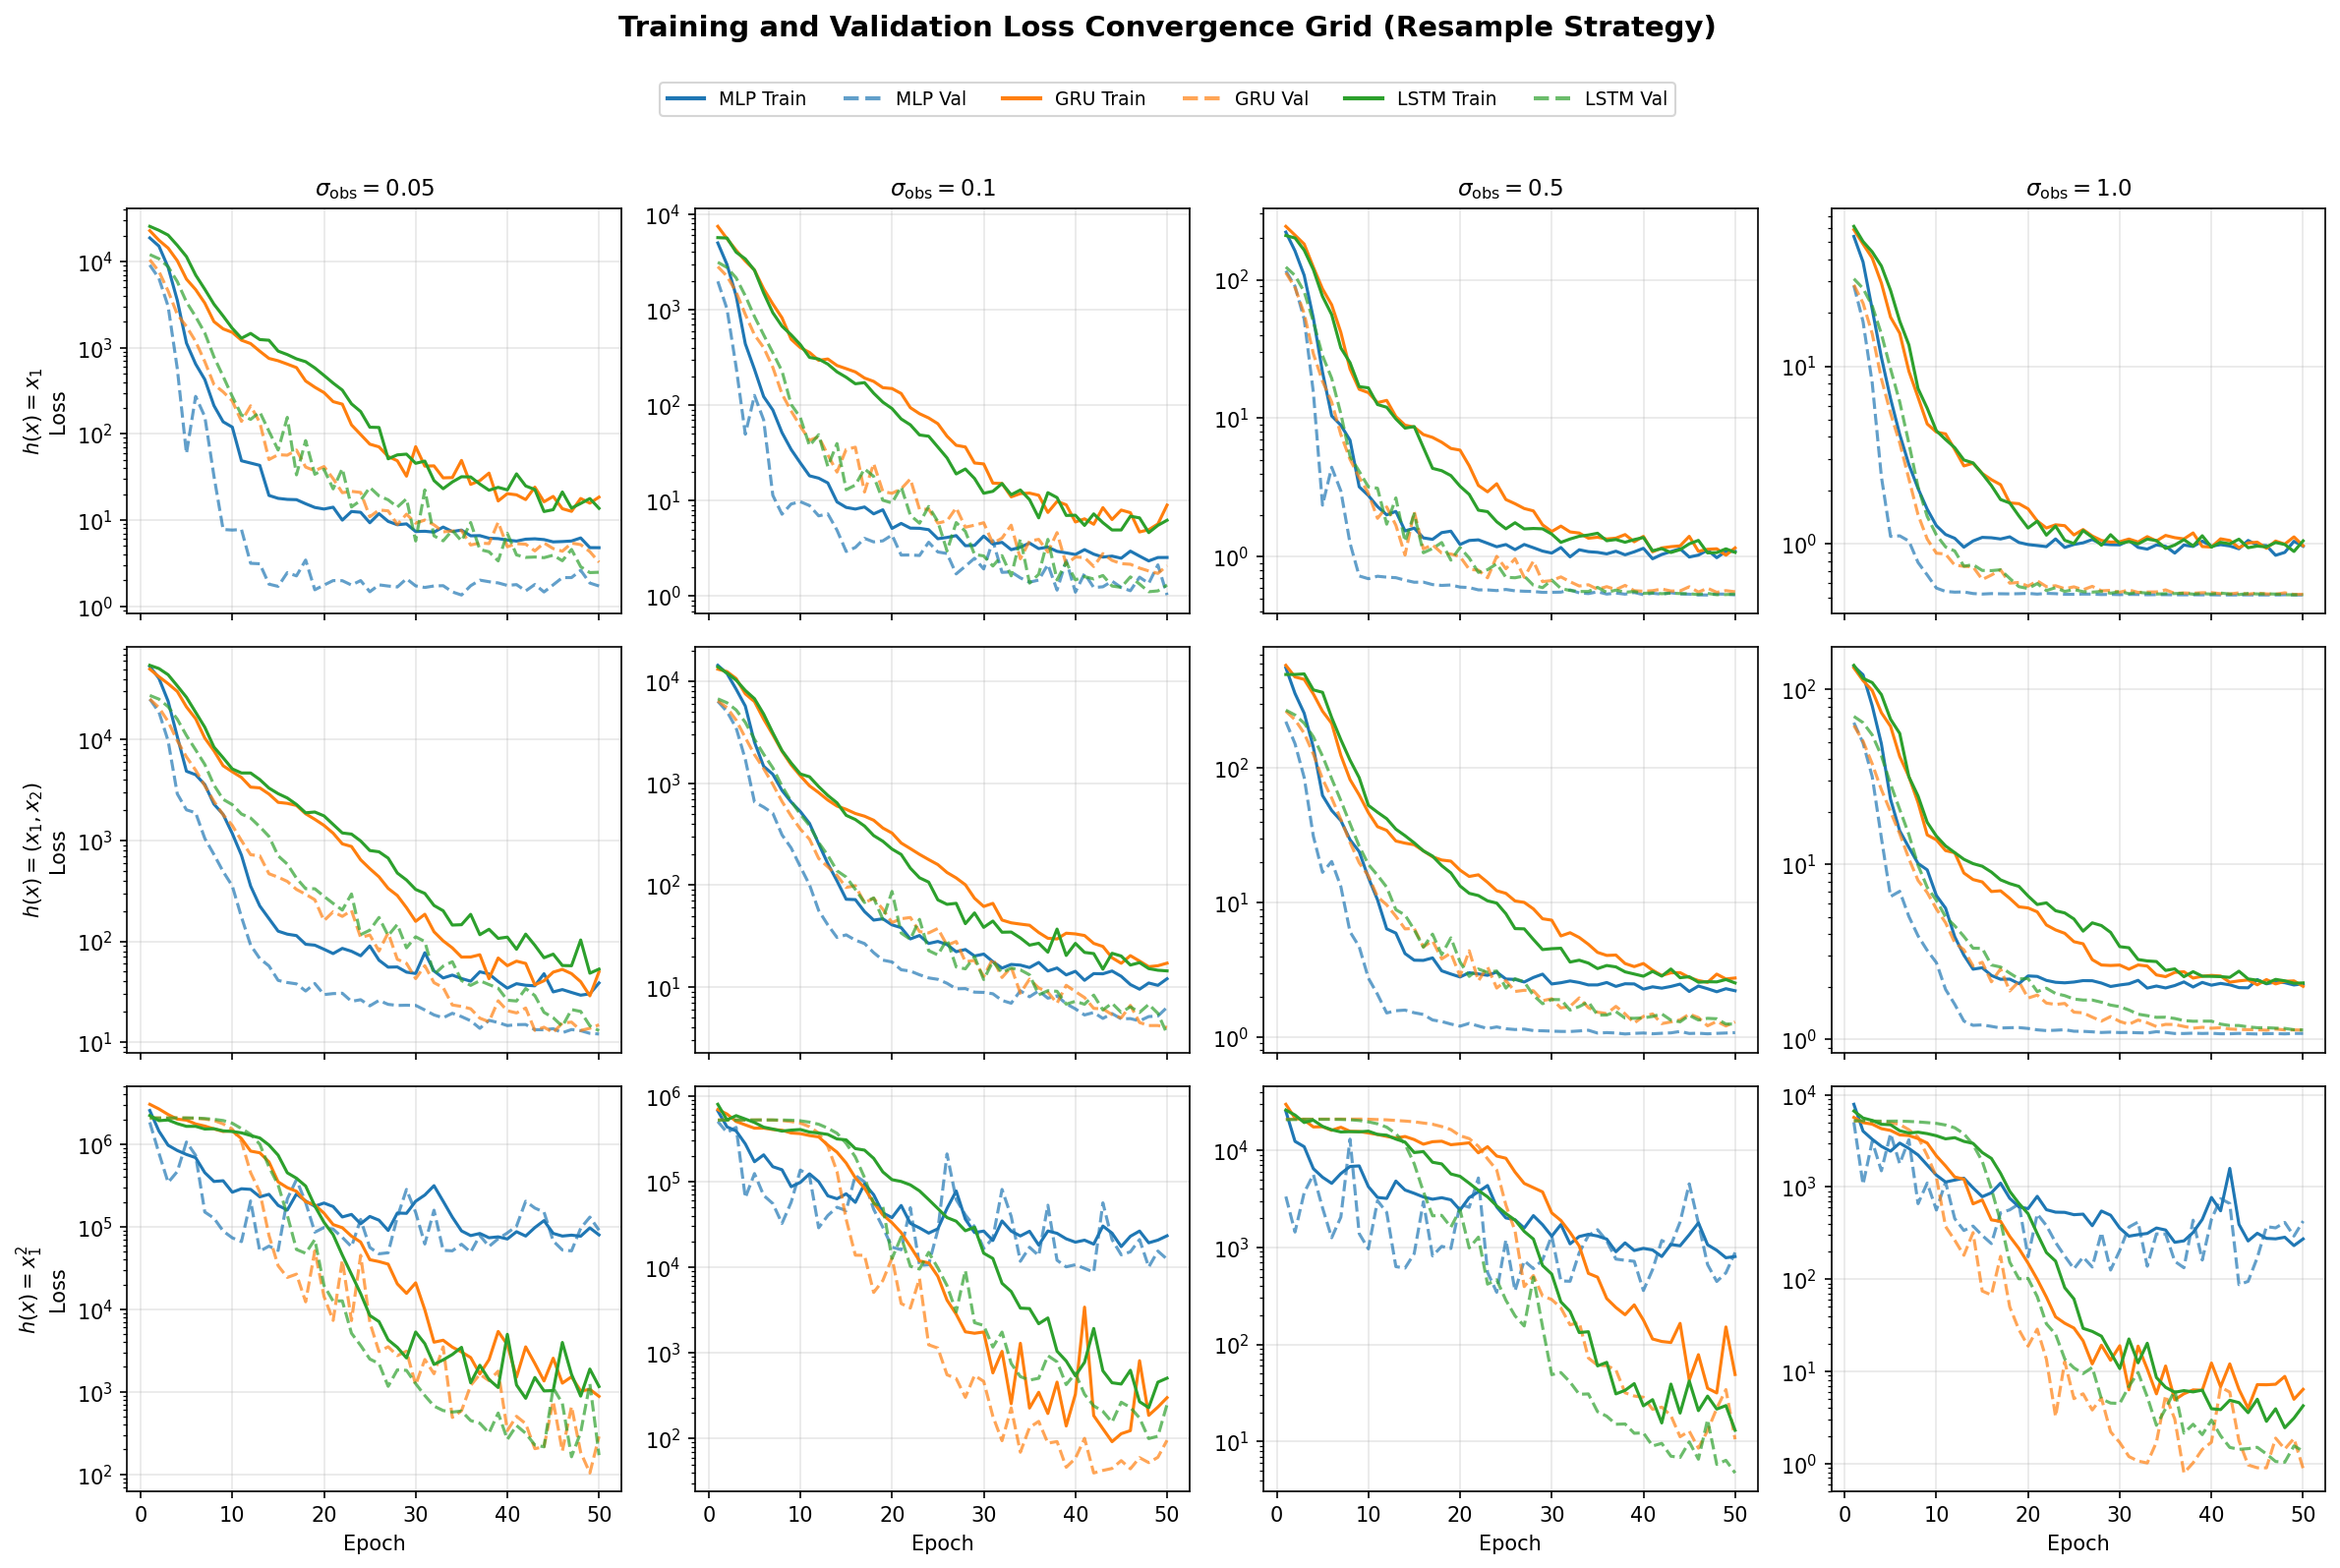
\includegraphics[width=\textwidth]{figures_new/training_validation_loss_grid.png}
\caption{(Appendix) Training and validation loss convergence grid for the Resample strategy. Rows correspond to observation modes ($h(x)=x_1$, $h(x)=(x_1,x_2)^\top$, $h(x)=x_1^2$); columns correspond to noise levels ($\sigma_{\text{obs}} \in \{0.05, 0.1, 0.5, 1.0\}$). Solid lines show training loss; dashed lines show validation loss. All architectures (MLP, GRU, LSTM) converge smoothly across all configurations.}
\label{fig:app_loss_grid}
\end{figure}

\newpage

\subsection*{A.3 Extended Attractor Geometry Diagnostics}
\addcontentsline{toc}{subsection}{A.3 Extended Attractor Geometry Diagnostics}
\label{sec:app_attractor}

This appendix provides comprehensive visual diagnostics for attractor geometry preservation, complementing the quantitative metrics presented in Section~\ref{sec:temporal}.

\subsubsection*{A.3.1 Phase-Space Projections and Hausdorff Metrics}

\begin{figure}[H]
\centering
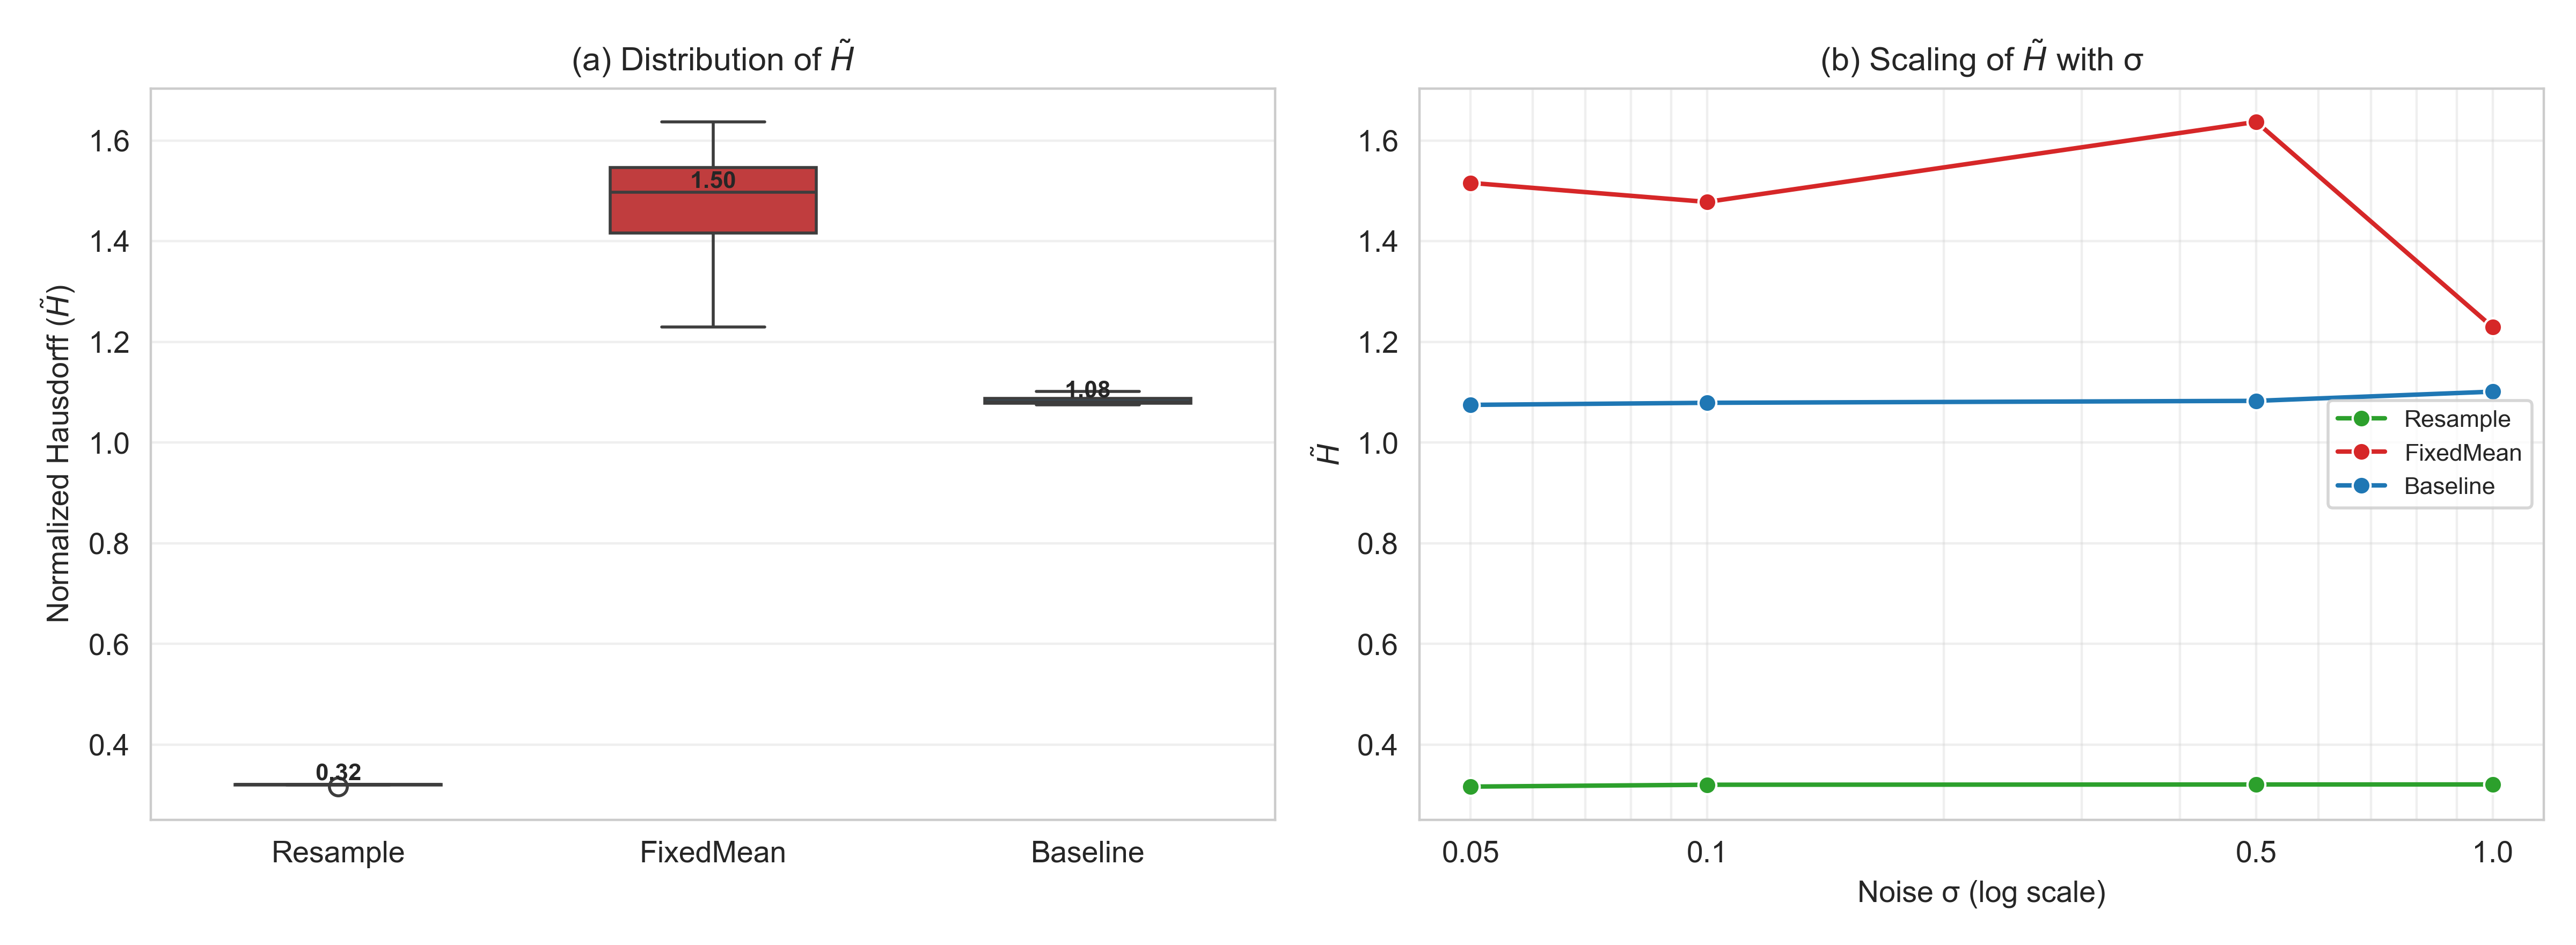
\includegraphics[width=\textwidth]{fig_attractor_geometry_side_by_side.png}
\caption{(Appendix) Phase--space projections (XY, YZ) for three assimilation strategies (Resample, FixedMean, Baseline) at two noise levels ($\sigma=0.1,0.5$). Each panel overlays truth (gray) and analysis (blue); inset text gives normalized Hausdorff distance $\tilde{H}$ where $\tilde{H}=H/\text{diam}(\mathcal{A}_{\text{truth}})$ and $H$ is the symmetric Hausdorff between truth and analysis trajectories (after downsampling to $\leq 6000$ points). Resample maintains close geometric adherence ($\tilde{H}\approx0.32$) across noise, Baseline drifts moderately ($\tilde{H}\approx1.11$), and FixedMean exhibits substantial structural distortion ($\tilde{H}\approx1.05$--1.64 depending on architecture).}
\label{fig:app_attractor_geometry_panels}
\end{figure}

\begin{figure}[H]
\centering
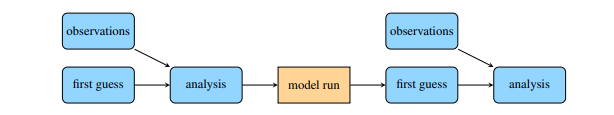
\includegraphics[width=0.92\textwidth]{fig_attractor_geometry_metrics.png}
\caption{(Appendix) (a) Distribution of normalized Hausdorff distances $\tilde{H}$ across noise levels ($\sigma\in\{0.05,0.1,0.5,1.0\}$) for each background conditioning strategy. (b) Scaling of $\tilde{H}$ with noise $\sigma$ (log scale). Medians (IQR): Resample $0.33$ (0.32--0.50), Baseline $1.11$ (1.10--1.13), FixedMean $1.39$ (1.14--1.52). Lower $\tilde{H}$ indicates better geometric adherence.}
\label{fig:app_attractor_geometry_metrics}
\end{figure}

\subsubsection*{A.3.2 Architecture-Specific Strategy Comparison}

\begin{figure}[H]
\centering
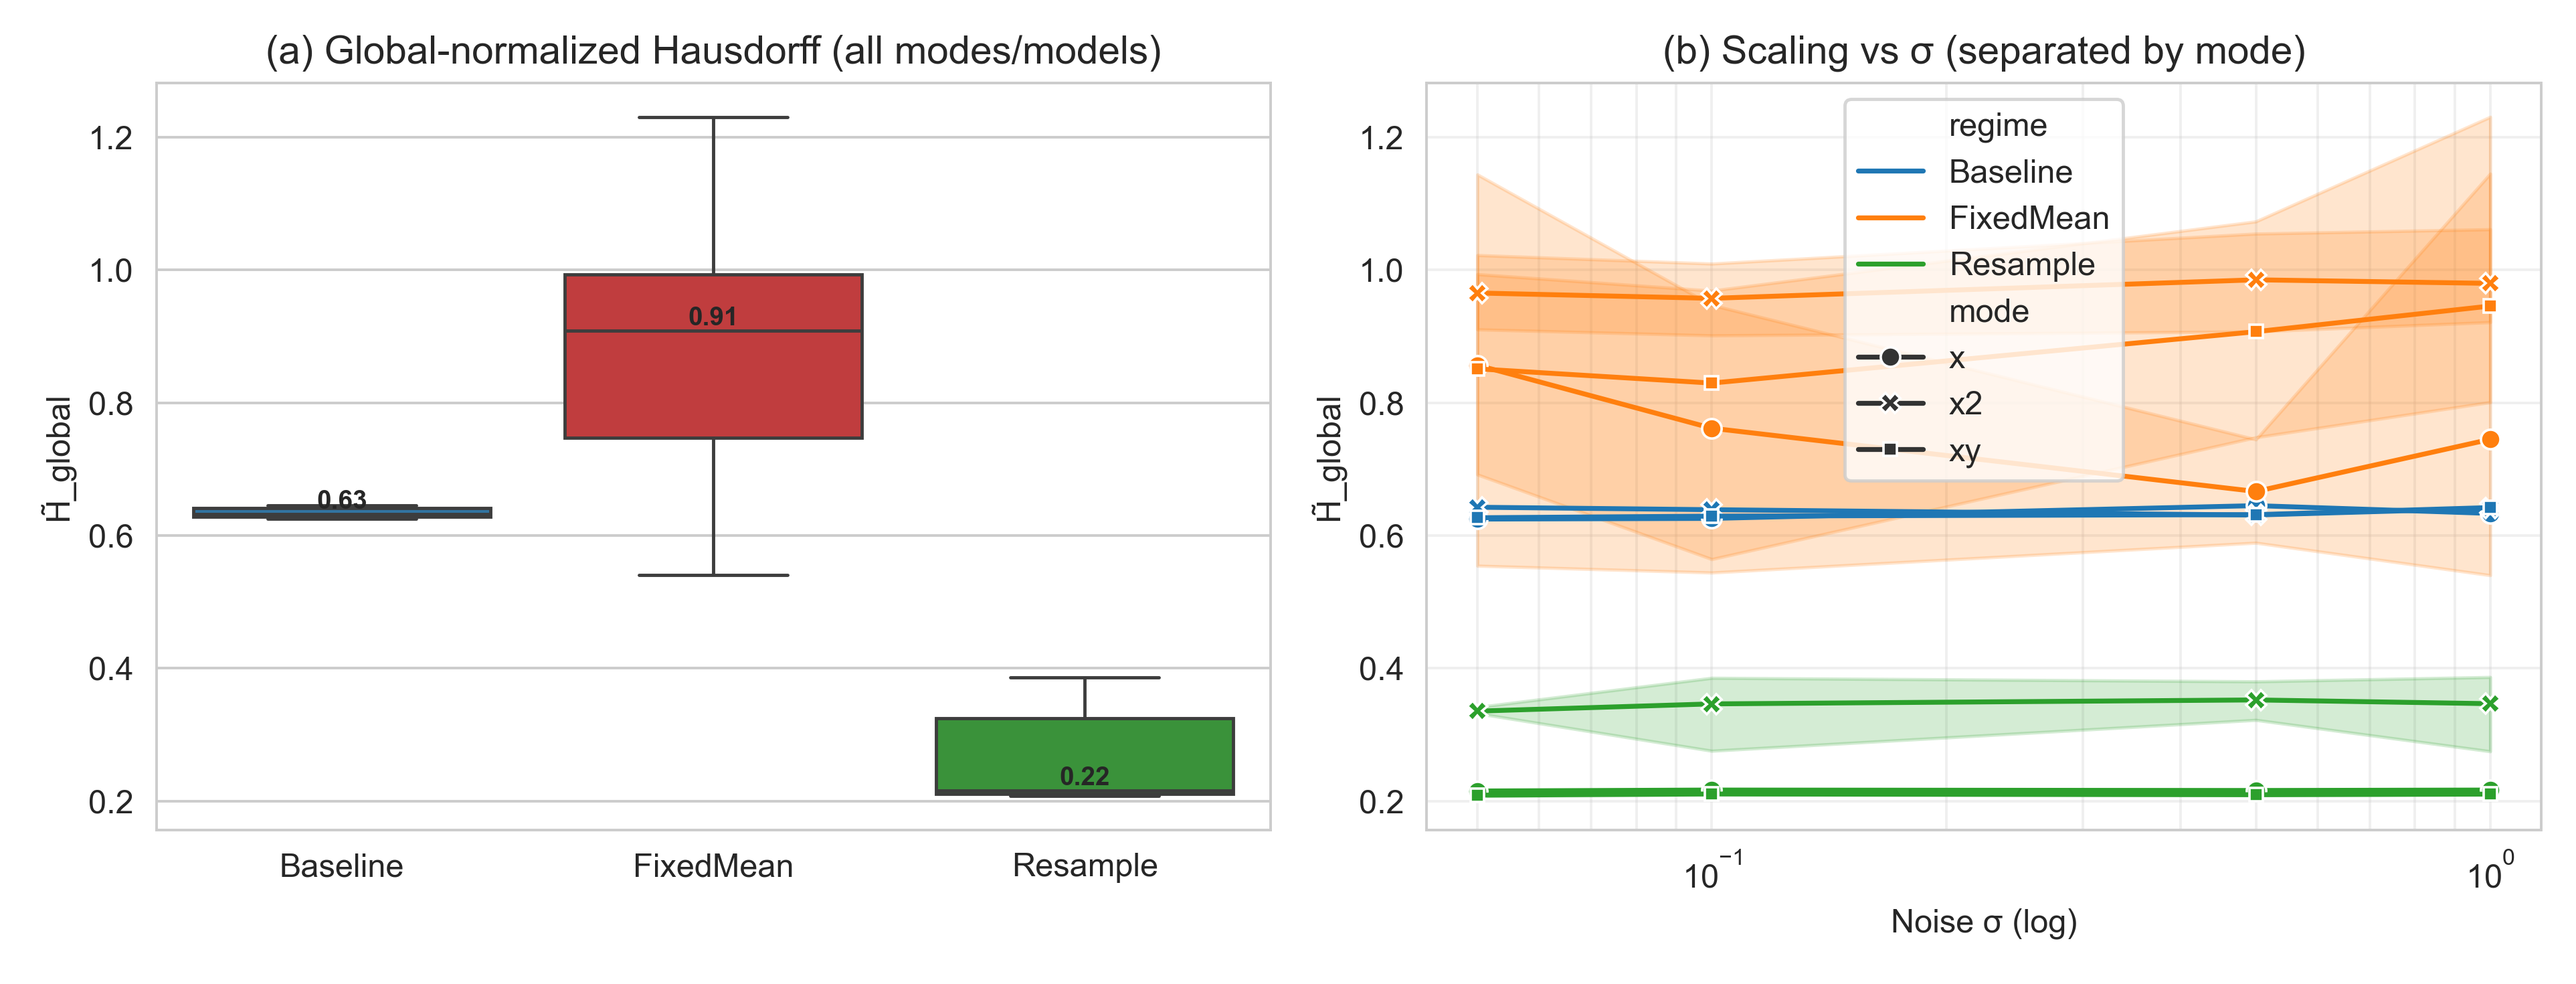
\includegraphics[width=0.92\textwidth]{attractor_metrics_resample_fixedmean.png}
\caption{(Appendix) Detailed comparison of global-normalized Hausdorff distances for Resample versus FixedMean strategies across architectures (MLP, GRU, LSTM) and noise levels. Left panel shows distributions at $\sigma=0.10$; right panel shows $\sigma=0.50$. Resample (blue) consistently outperforms FixedMean (red) across all architectures, with GRU and LSTM showing slight advantages in noise resilience. At higher noise ($\sigma=0.50$), FixedMean distributions broaden significantly, indicating geometric instability, while Resample remains tightly concentrated near $\tilde{H}_{\text{global}} \approx 0.32$. This confirms that architectural choice is secondary to background conditioning strategy selection: dynamic background updates are the primary driver of geometric fidelity.}
\label{fig:app_attractor_metrics_detailed}
\end{figure}

\subsubsection*{A.3.2b Lobe Occupancy Analysis}

The lobe occupancy discrepancy $\Delta_{\text{lobe}}$ validates global topology preservation.

\begin{figure}[H]
\centering
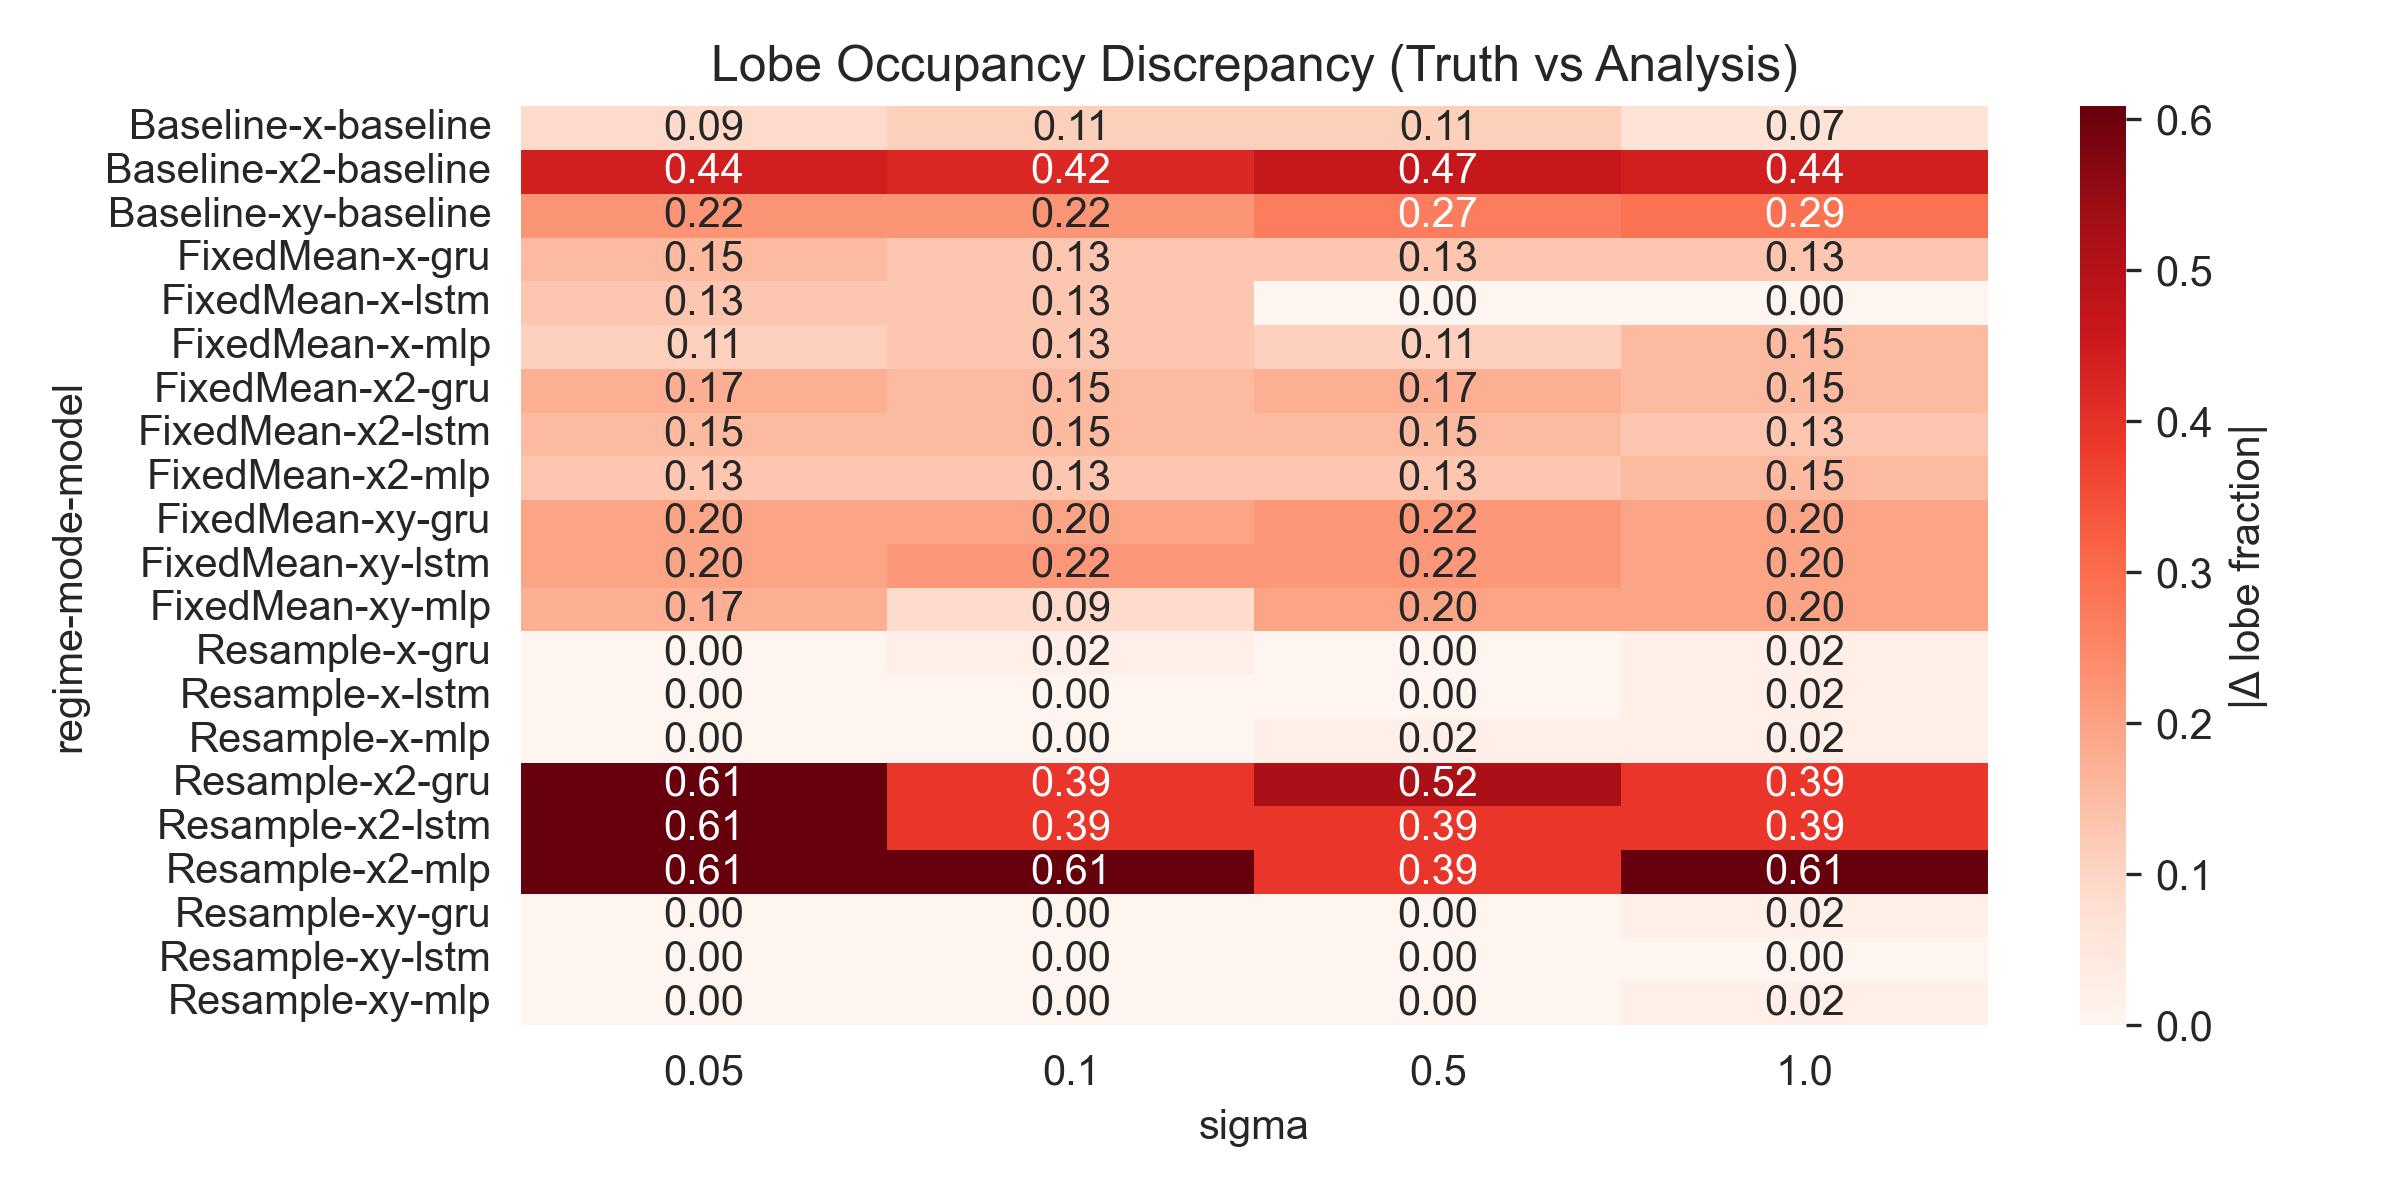
\includegraphics[width=\textwidth]{lobe_occupancy_diff_heatmap.png}
\caption{Lobe occupancy discrepancy ($\Delta_{\text{lobe}}$) for all strategies and observation modes across noise levels. Light cells indicate near-perfect lobe matching ($\Delta_{\text{lobe}} \approx 0$); dark cells indicate substantial imbalance. For linear modes ($h(x)=x_1$ and $h(x)=(x_1,x_2)^\top$), Resample achieves low discrepancies ($\Delta_{\text{lobe}} < 0.02$), indicating correct separatrix crossings. The nonlinear $h(x)=x_1^2$ mode produces high discrepancies for all strategies because the quadratic observation removes sign information. FixedMean shows moderate bias ($\Delta_{\text{lobe}} \approx 0.10$--0.22) across $x$ and $xy$ modes.}
\label{fig:lobe_discrepancy}
\end{figure}

\noindent
Resample achieves near-zero lobe occupancy discrepancy ($\Delta_{\text{lobe}} < 0.02$) for the linear observation modes ($h(x) = x_1$ and $h(x) = (x_1, x_2)^\top$), confirming that dynamic background updates enable correct separatrix crossing and balanced wing visitation. Under the nonlinear $h(x) = x_1^2$ mode, lobe balance cannot be recovered by any background strategy: Resample gives $\Delta_{\text{lobe}} \approx 0.39$--0.61, Baseline $\approx 0.42$--0.47, and FixedMean $\approx 0.13$--0.17. The low FixedMean values here reflect near-fixed-point trajectories that spuriously maintain symmetric lobe counts rather than correct chaotic dynamics. For $x$ and $xy$ modes, FixedMean exhibits lobe imbalances at higher noise, with approximately 13\% discrepancy at $\sigma_{\text{obs}} = 0.50$ under the $x$ mode.

\subsubsection*{A.3.3 Multi-Strategy Attractor Grids}

% =====================================================
% BASELINE
% =====================================================

\begin{figure}[H]
\centering

\includegraphics[width=\textwidth, keepaspectratio]{ATTRACTOR_GRID_Baseline_x.png}
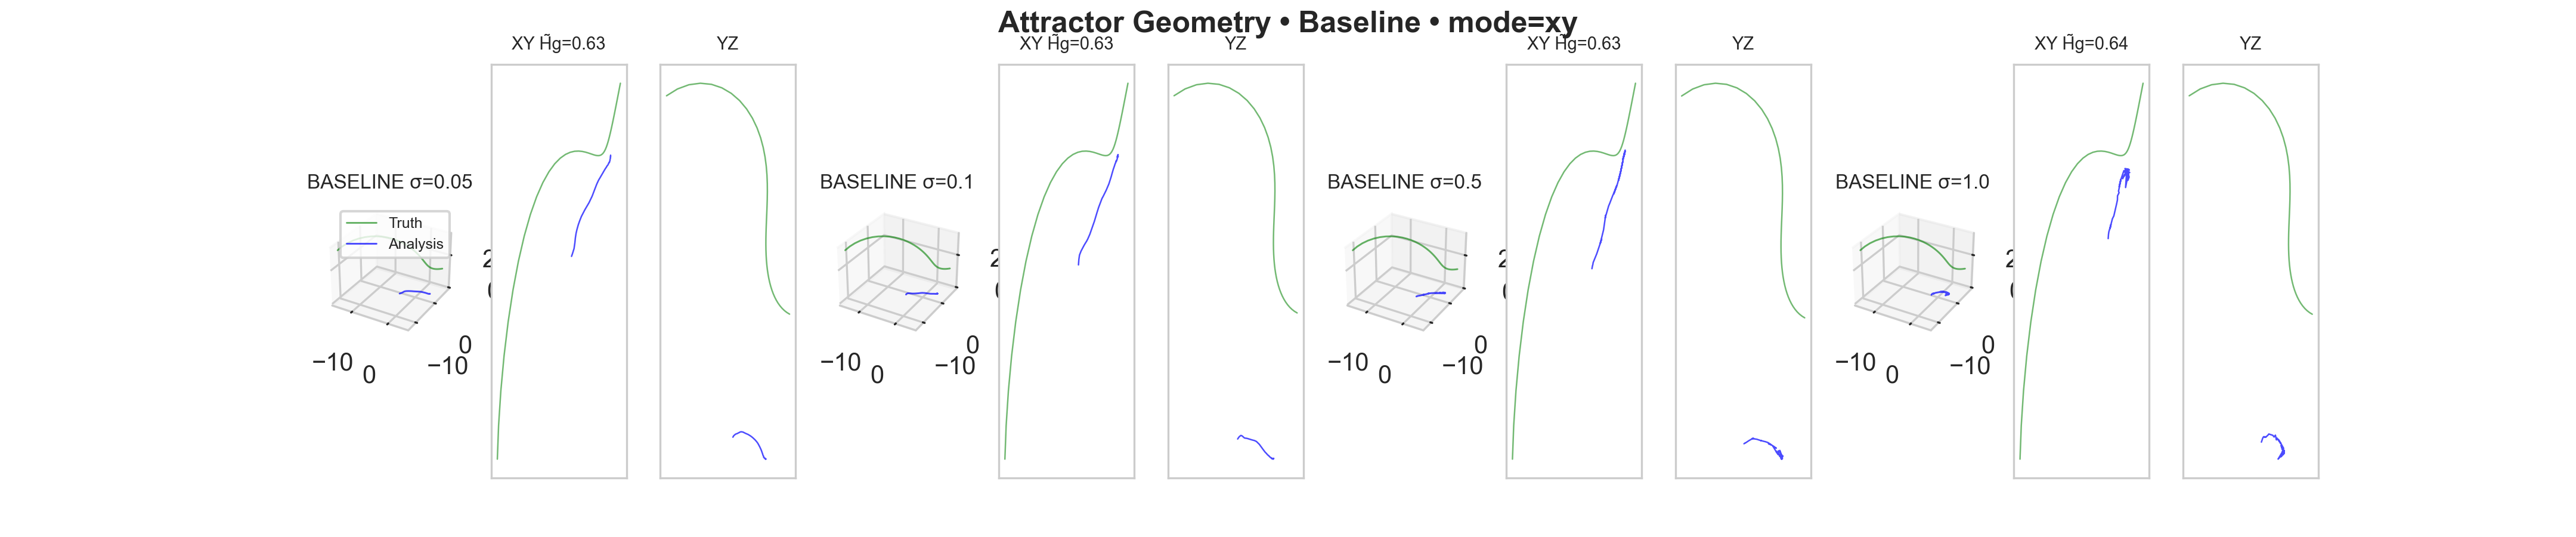
\includegraphics[width=\textwidth, keepaspectratio]{ATTRACTOR_GRID_Baseline_xy.png}
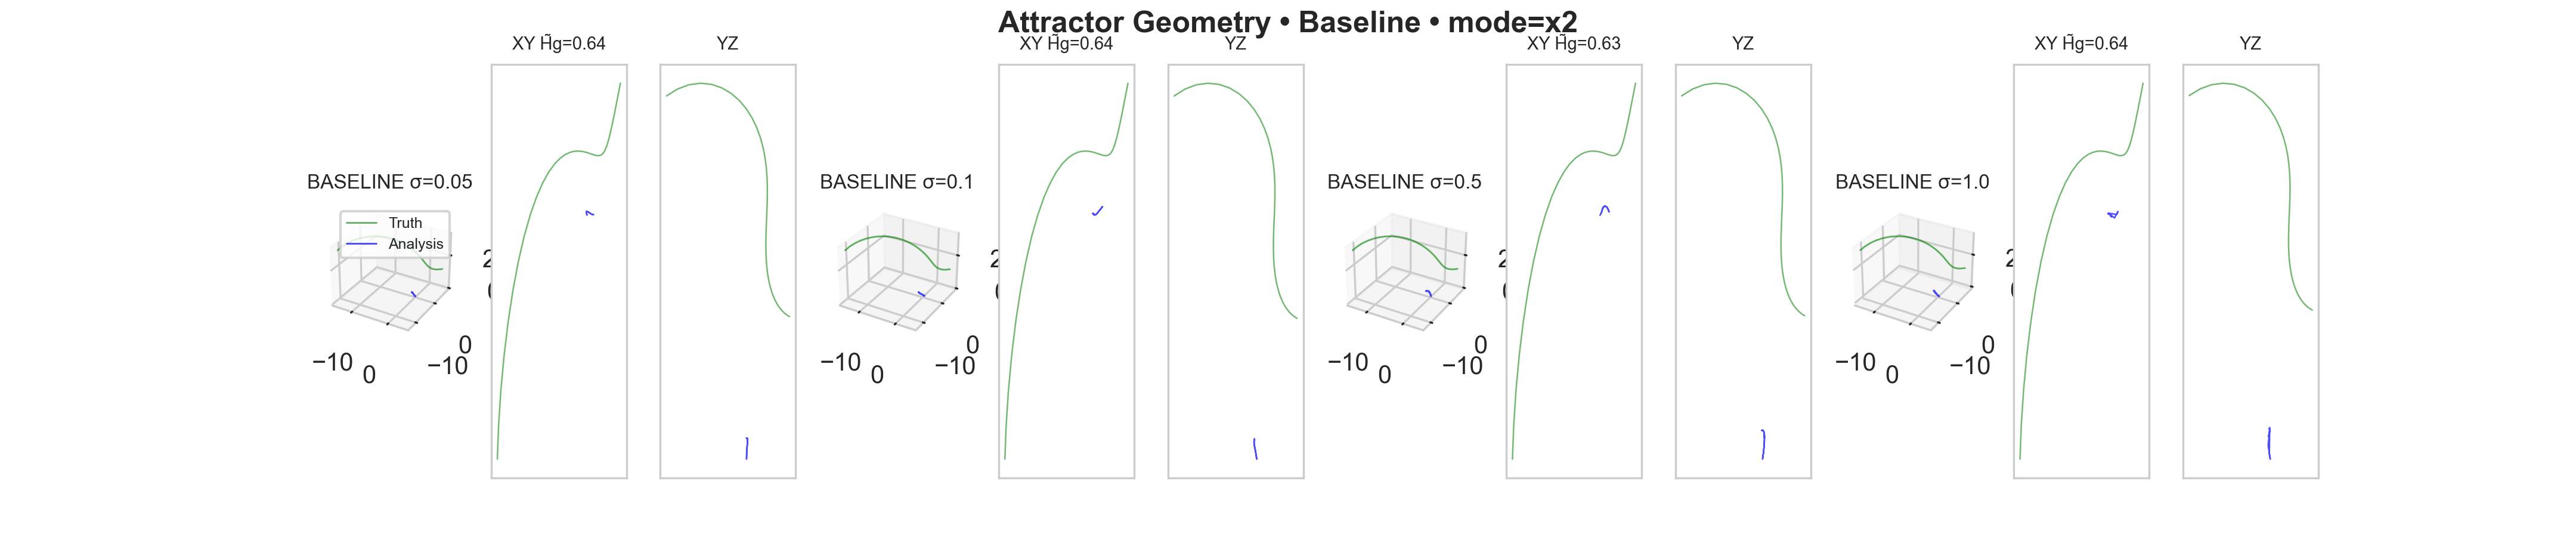
\includegraphics[width=\textwidth, keepaspectratio]{ATTRACTOR_GRID_Baseline_x2.png}
\caption{(Appendix) Attractor geometry for the Baseline strategy across three observation modes ($x$, $xy$, and $x^2$) and four noise levels ($\sigma \in \{0.05, 0.10, 0.50, 1.00\}$). Each grid contains XY and YZ projections with truth (gray) and analysis (blue) trajectories. Baseline maintains partial geometric fidelity at low noise but exhibits increasing lobe imbalance and drift at higher noise, particularly for the $x^2$ mode where nonlinear observations reduce separatrix information.}
\label{fig:app_attractor_grid_baseline}
\end{figure}

% =====================================================
% FIXEDMEAN
% =====================================================

\begin{figure}[H]
\centering
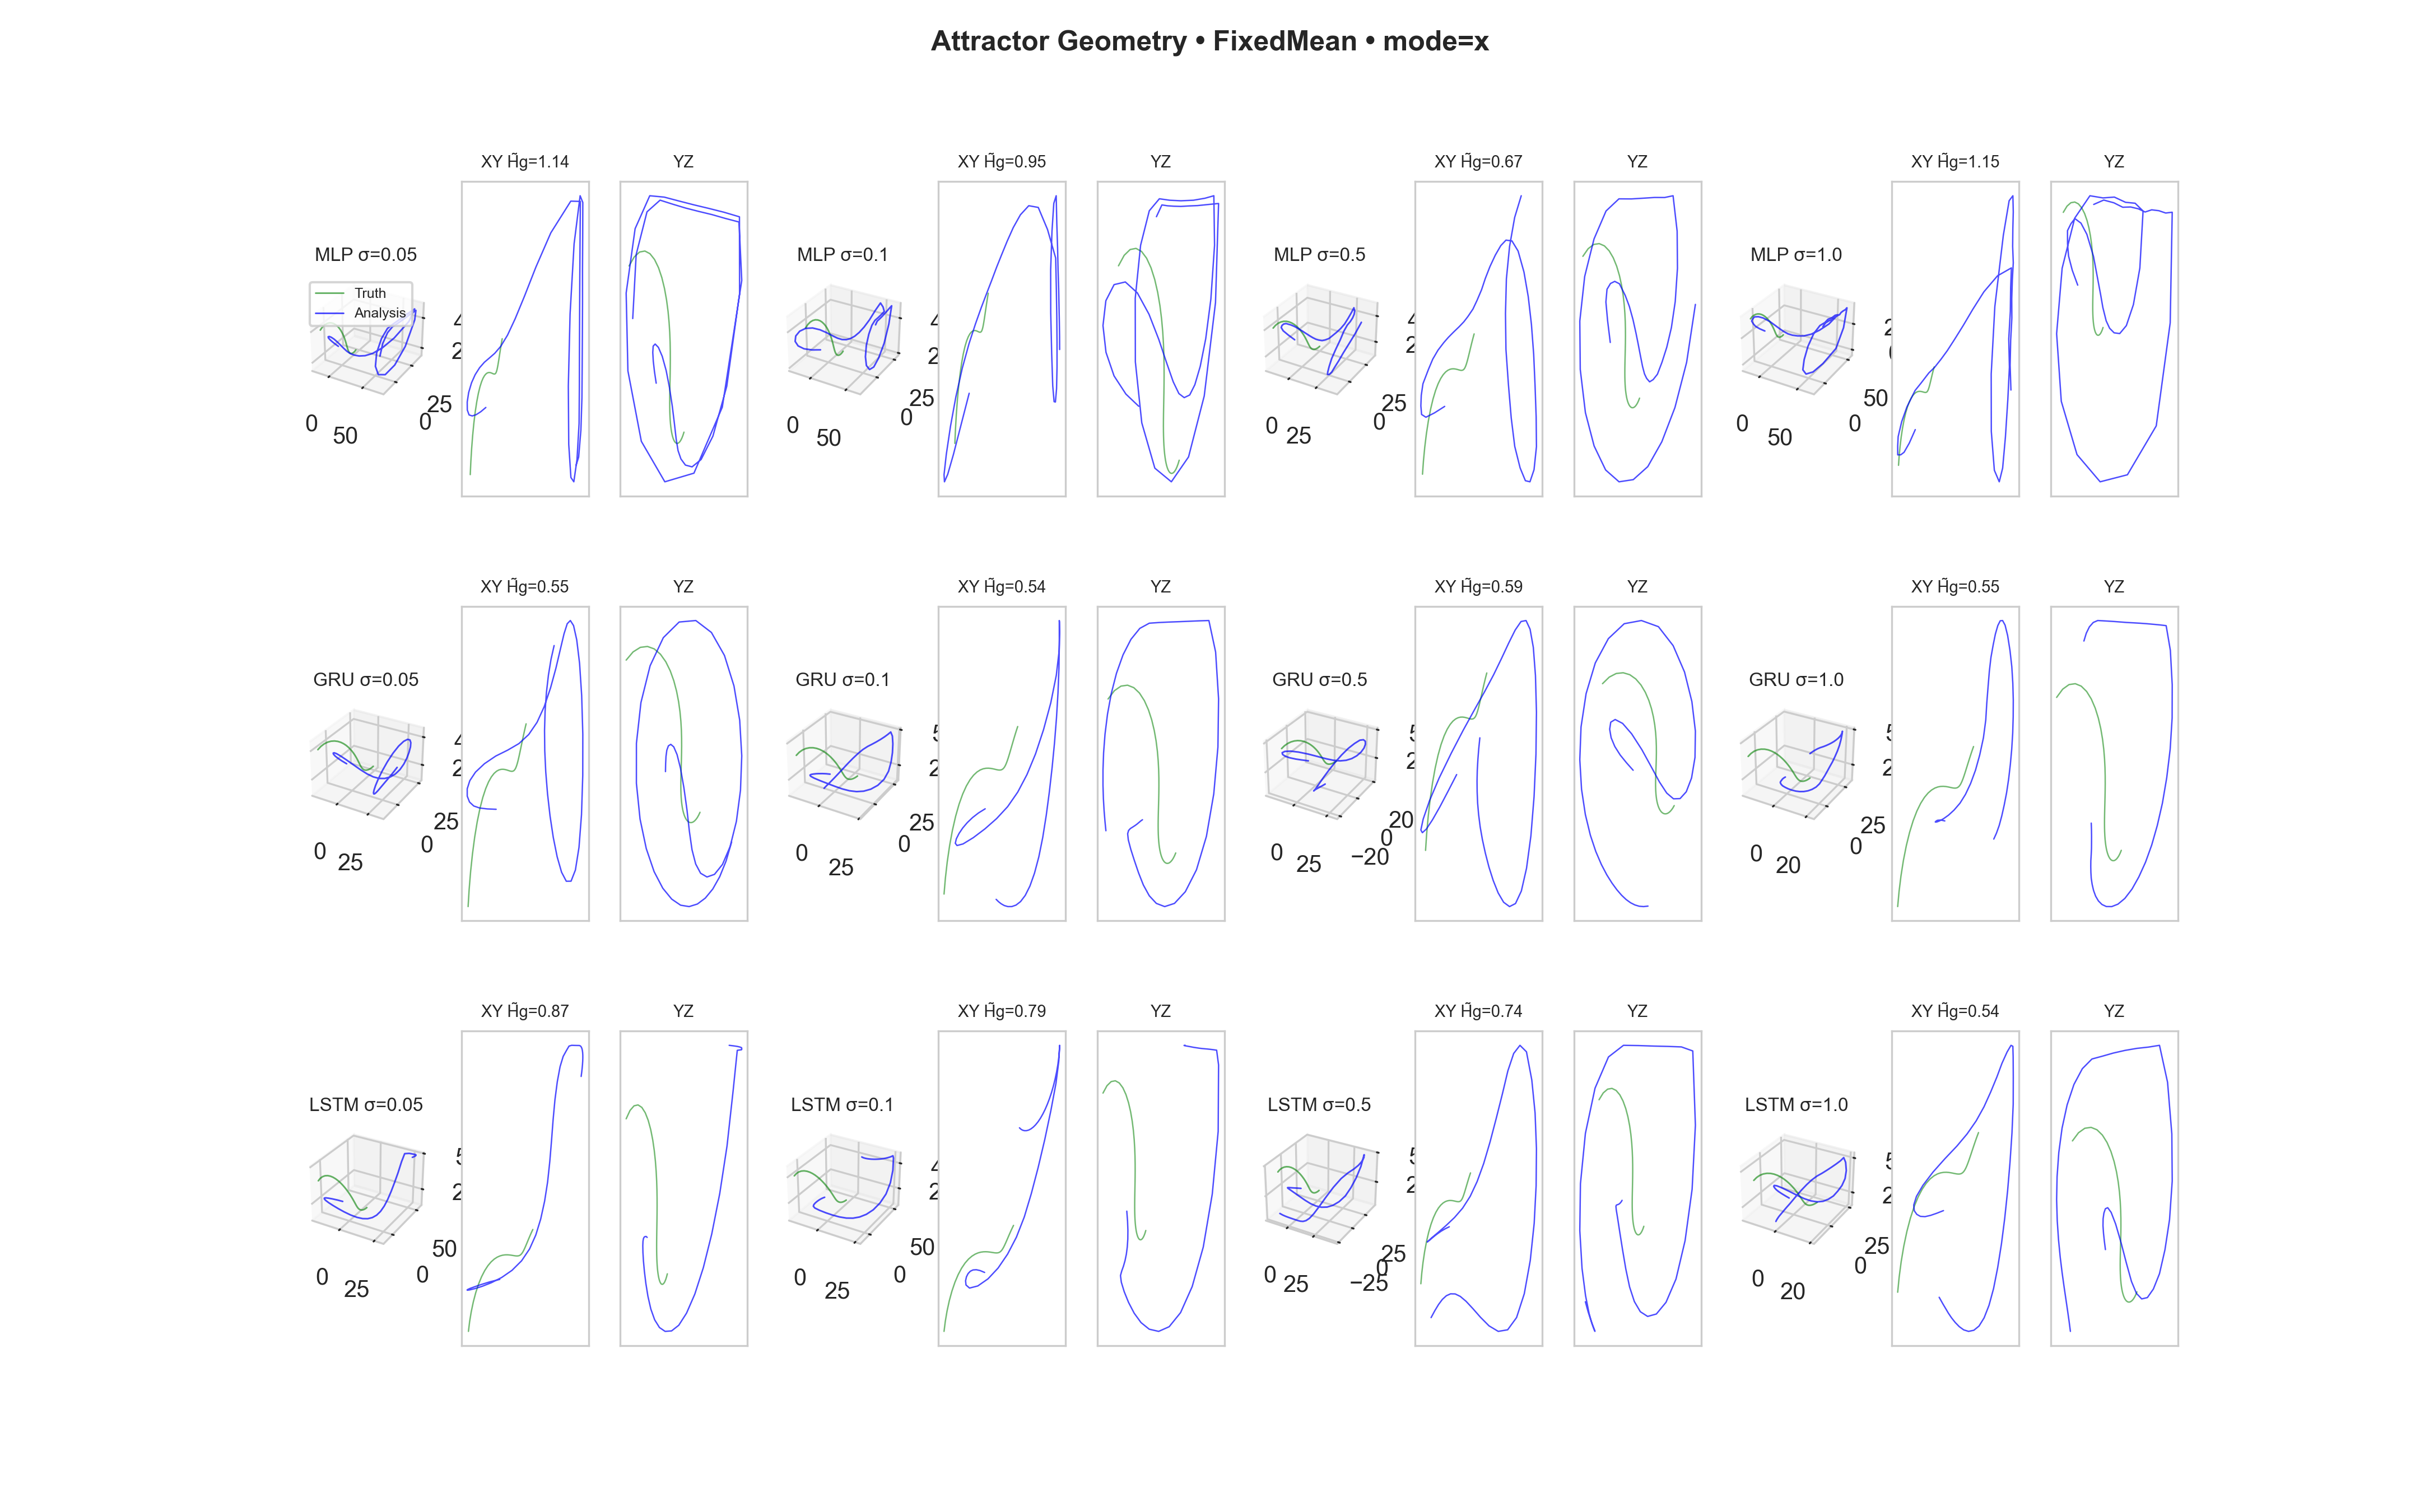
\includegraphics[width=\textwidth, keepaspectratio]{ATTRACTOR_GRID_FixedMean_x.png}
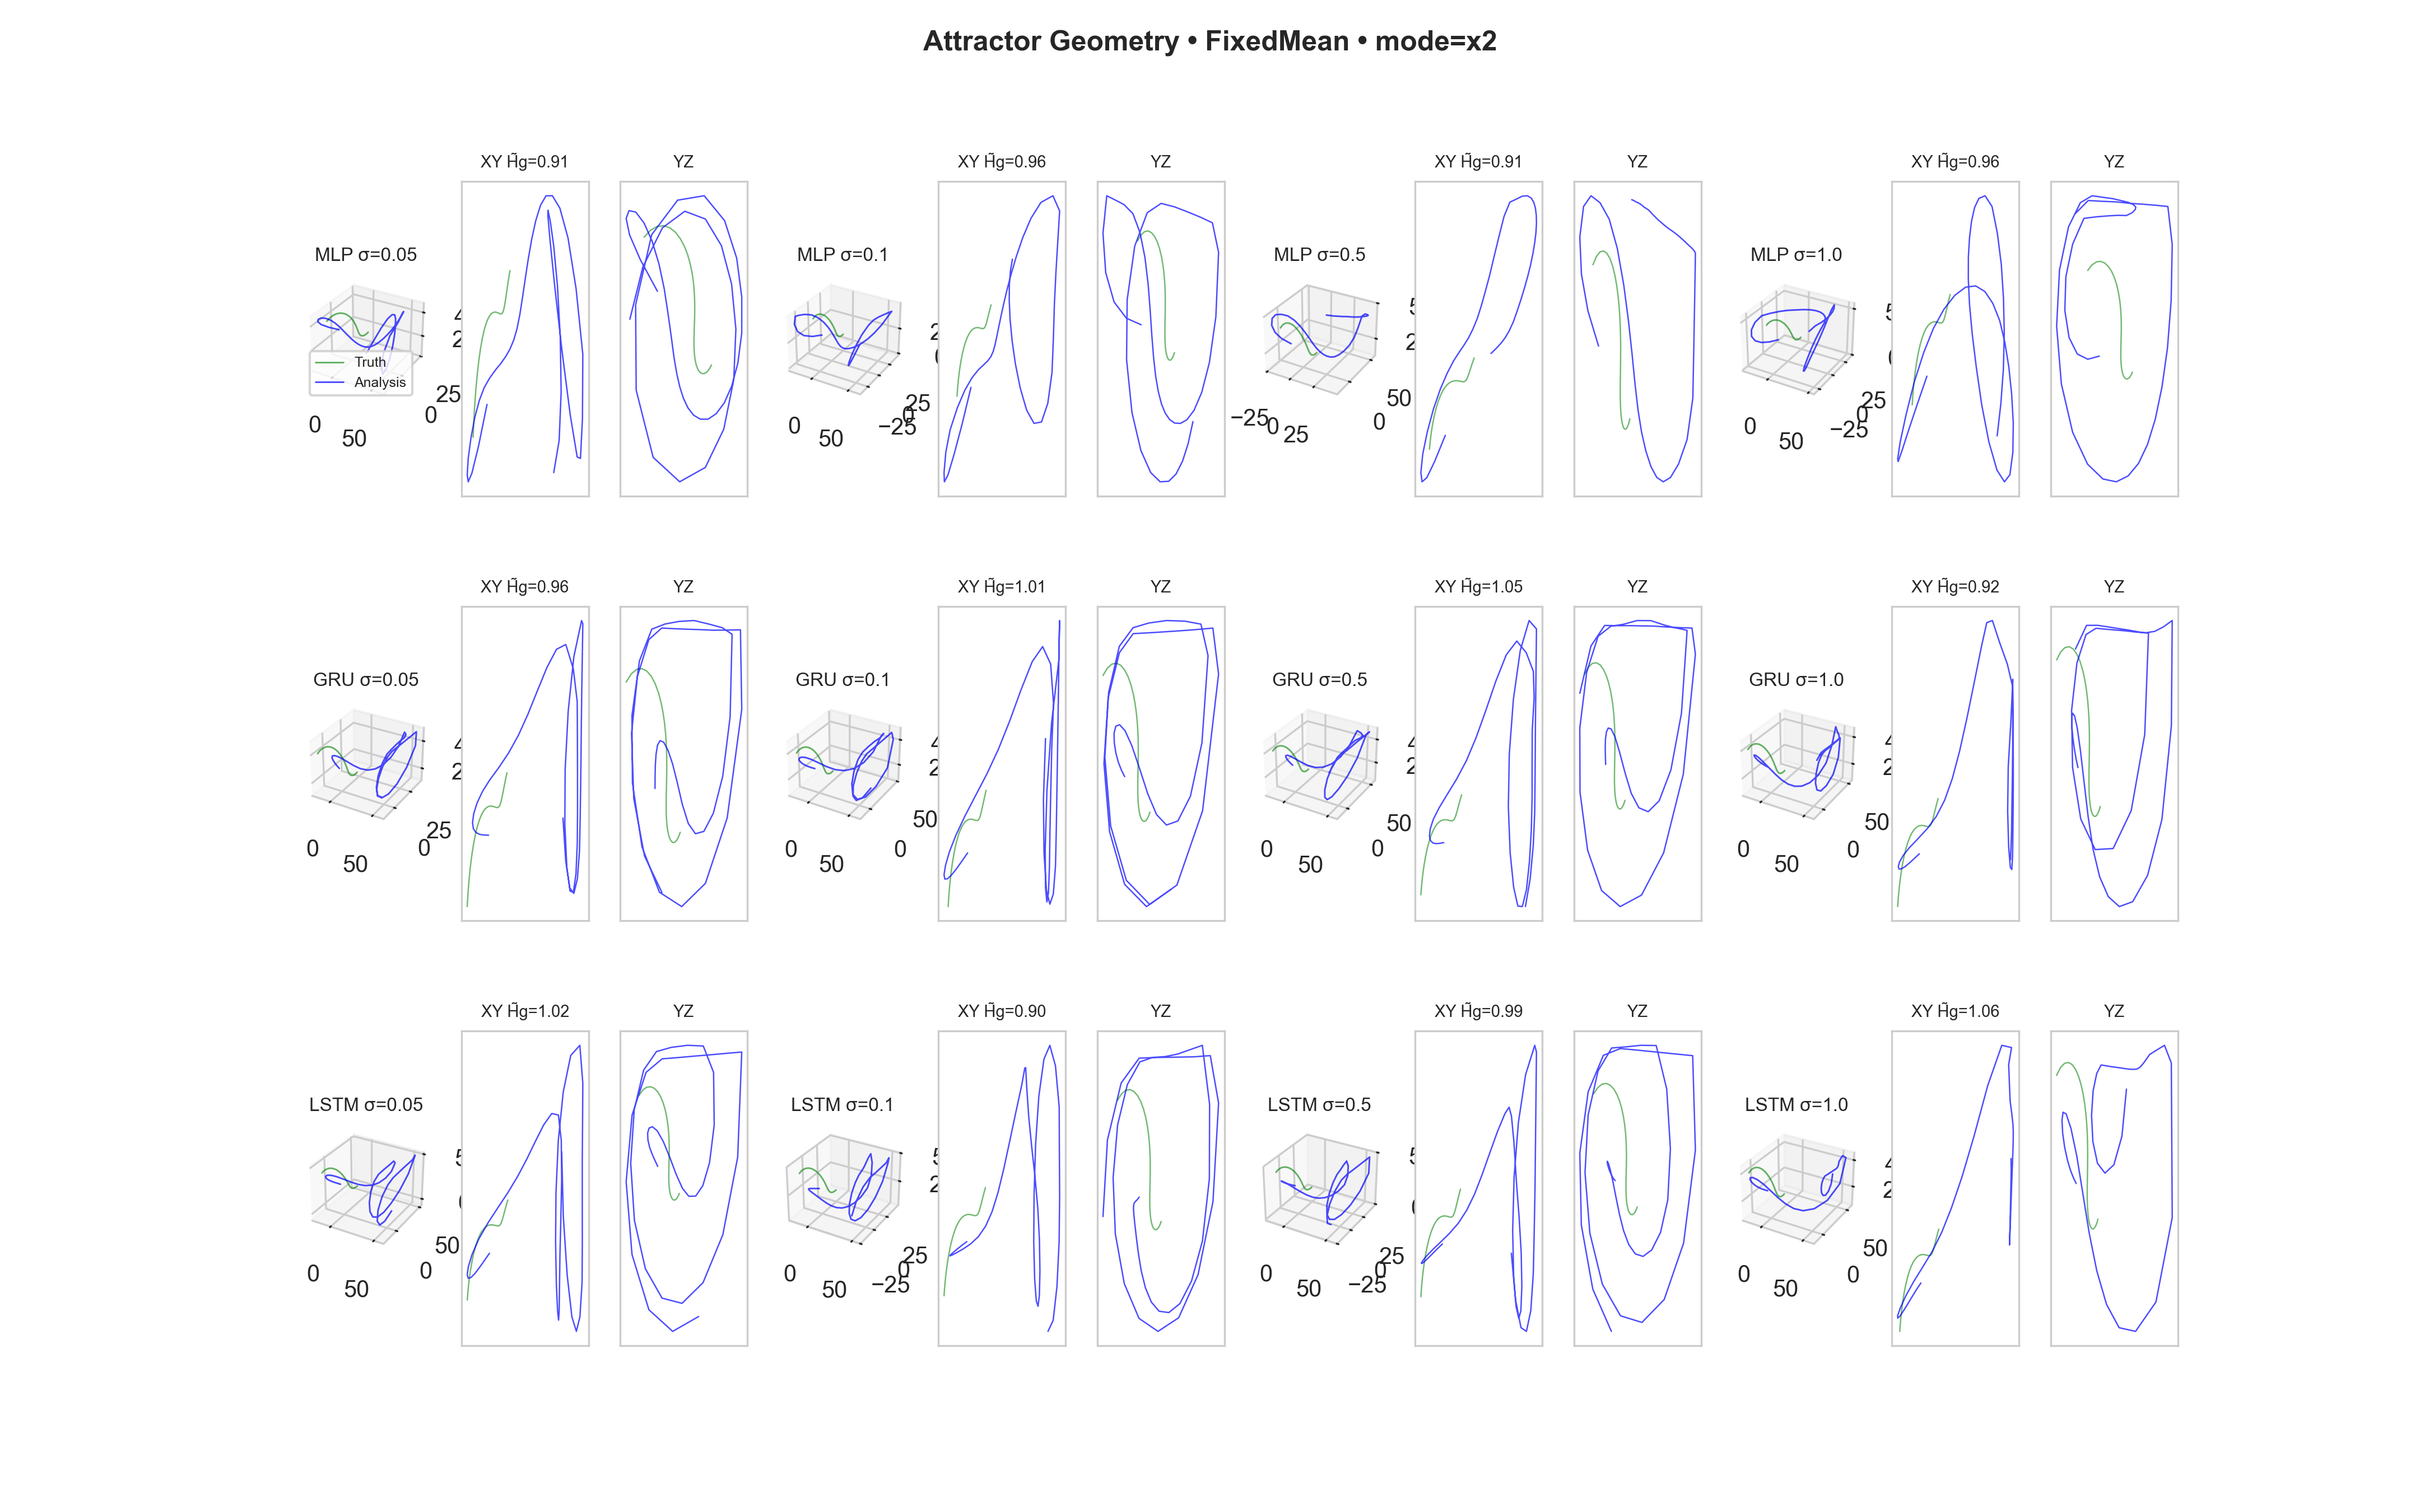
\includegraphics[width=\textwidth, keepaspectratio]{ATTRACTOR_GRID_FixedMean_xy.png}
\end{figure}
\begin{figure}[H]
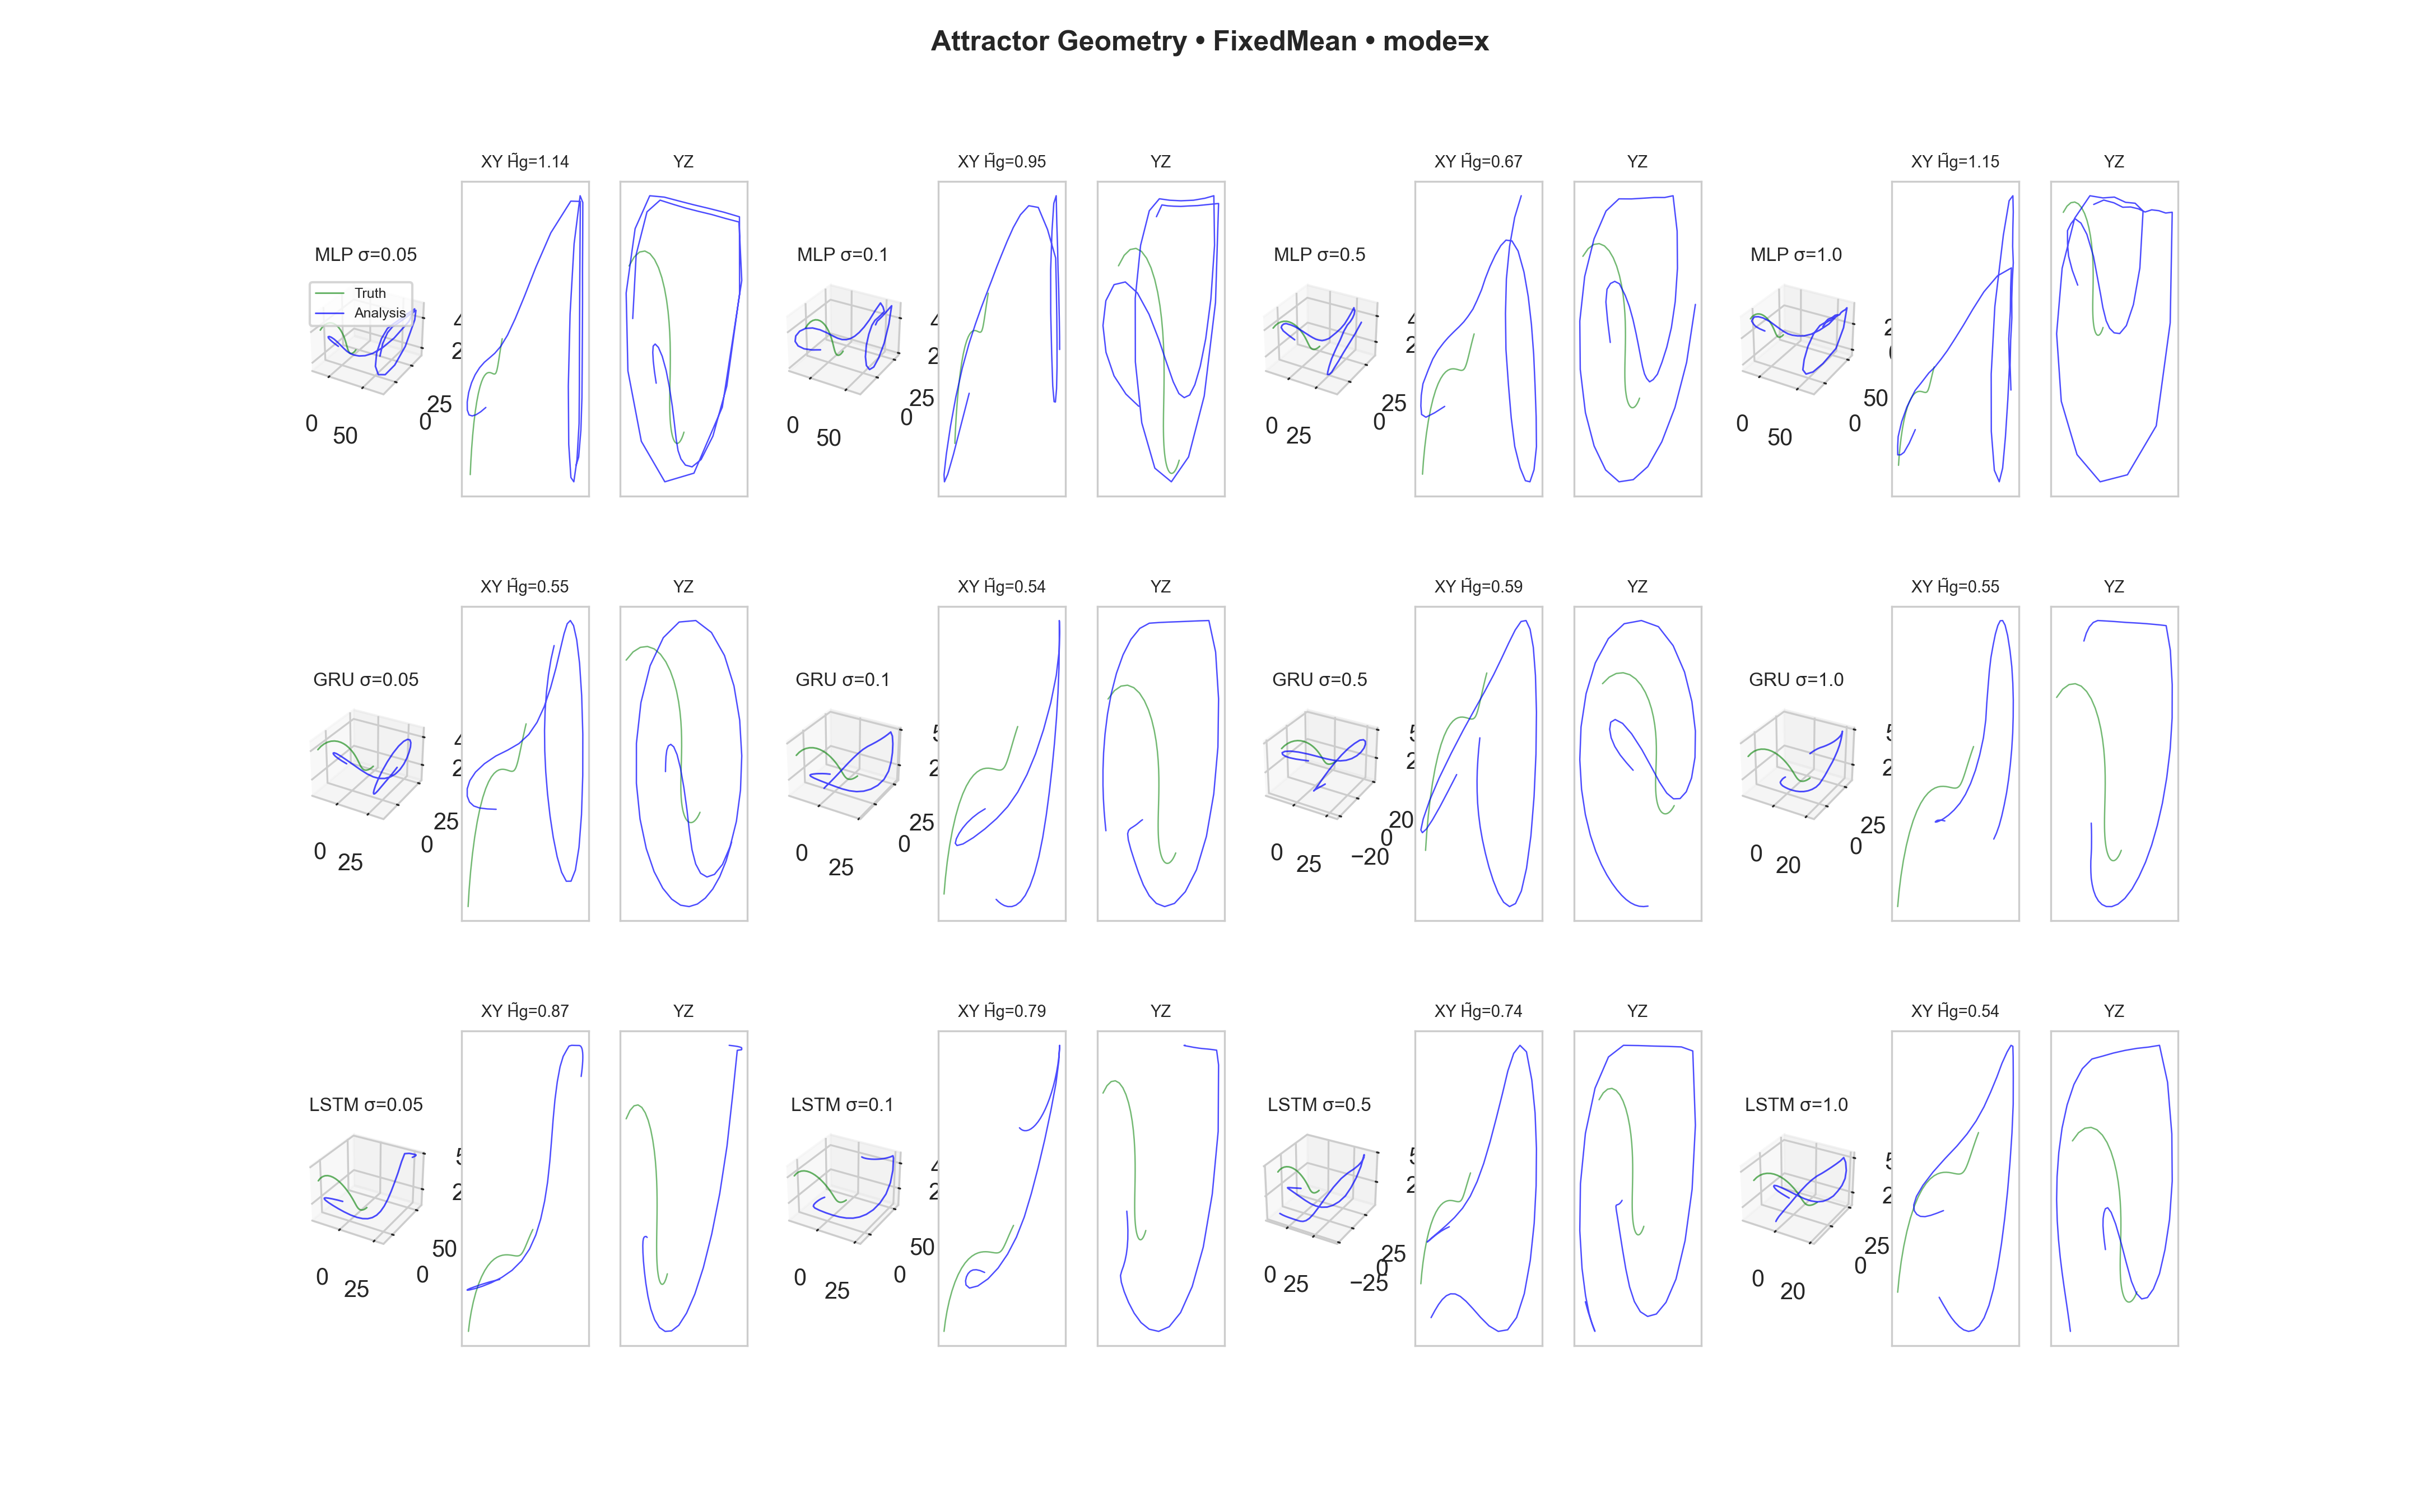
\includegraphics[width=\textwidth, keepaspectratio]{ATTRACTOR_GRID_FixedMean_x2.png}
\caption{(Appendix) Attractor geometry for the FixedMean strategy across observation modes. FixedMean displays substantial geometric degradation at moderate and high noise levels. Analysis trajectories (blue) deviate from truth (gray), often collapsing toward fixed points or producing fragmented, non-chaotic shapes. These distortions are consistent with the elevated lobe imbalance values observed in Fig.~\ref{fig:lobe_discrepancy}.}
\label{fig:app_attractor_grid_fixedmean}
\end{figure}


% =====================================================
% RESAMPLE
% =====================================================

\begin{figure}[H]
\centering
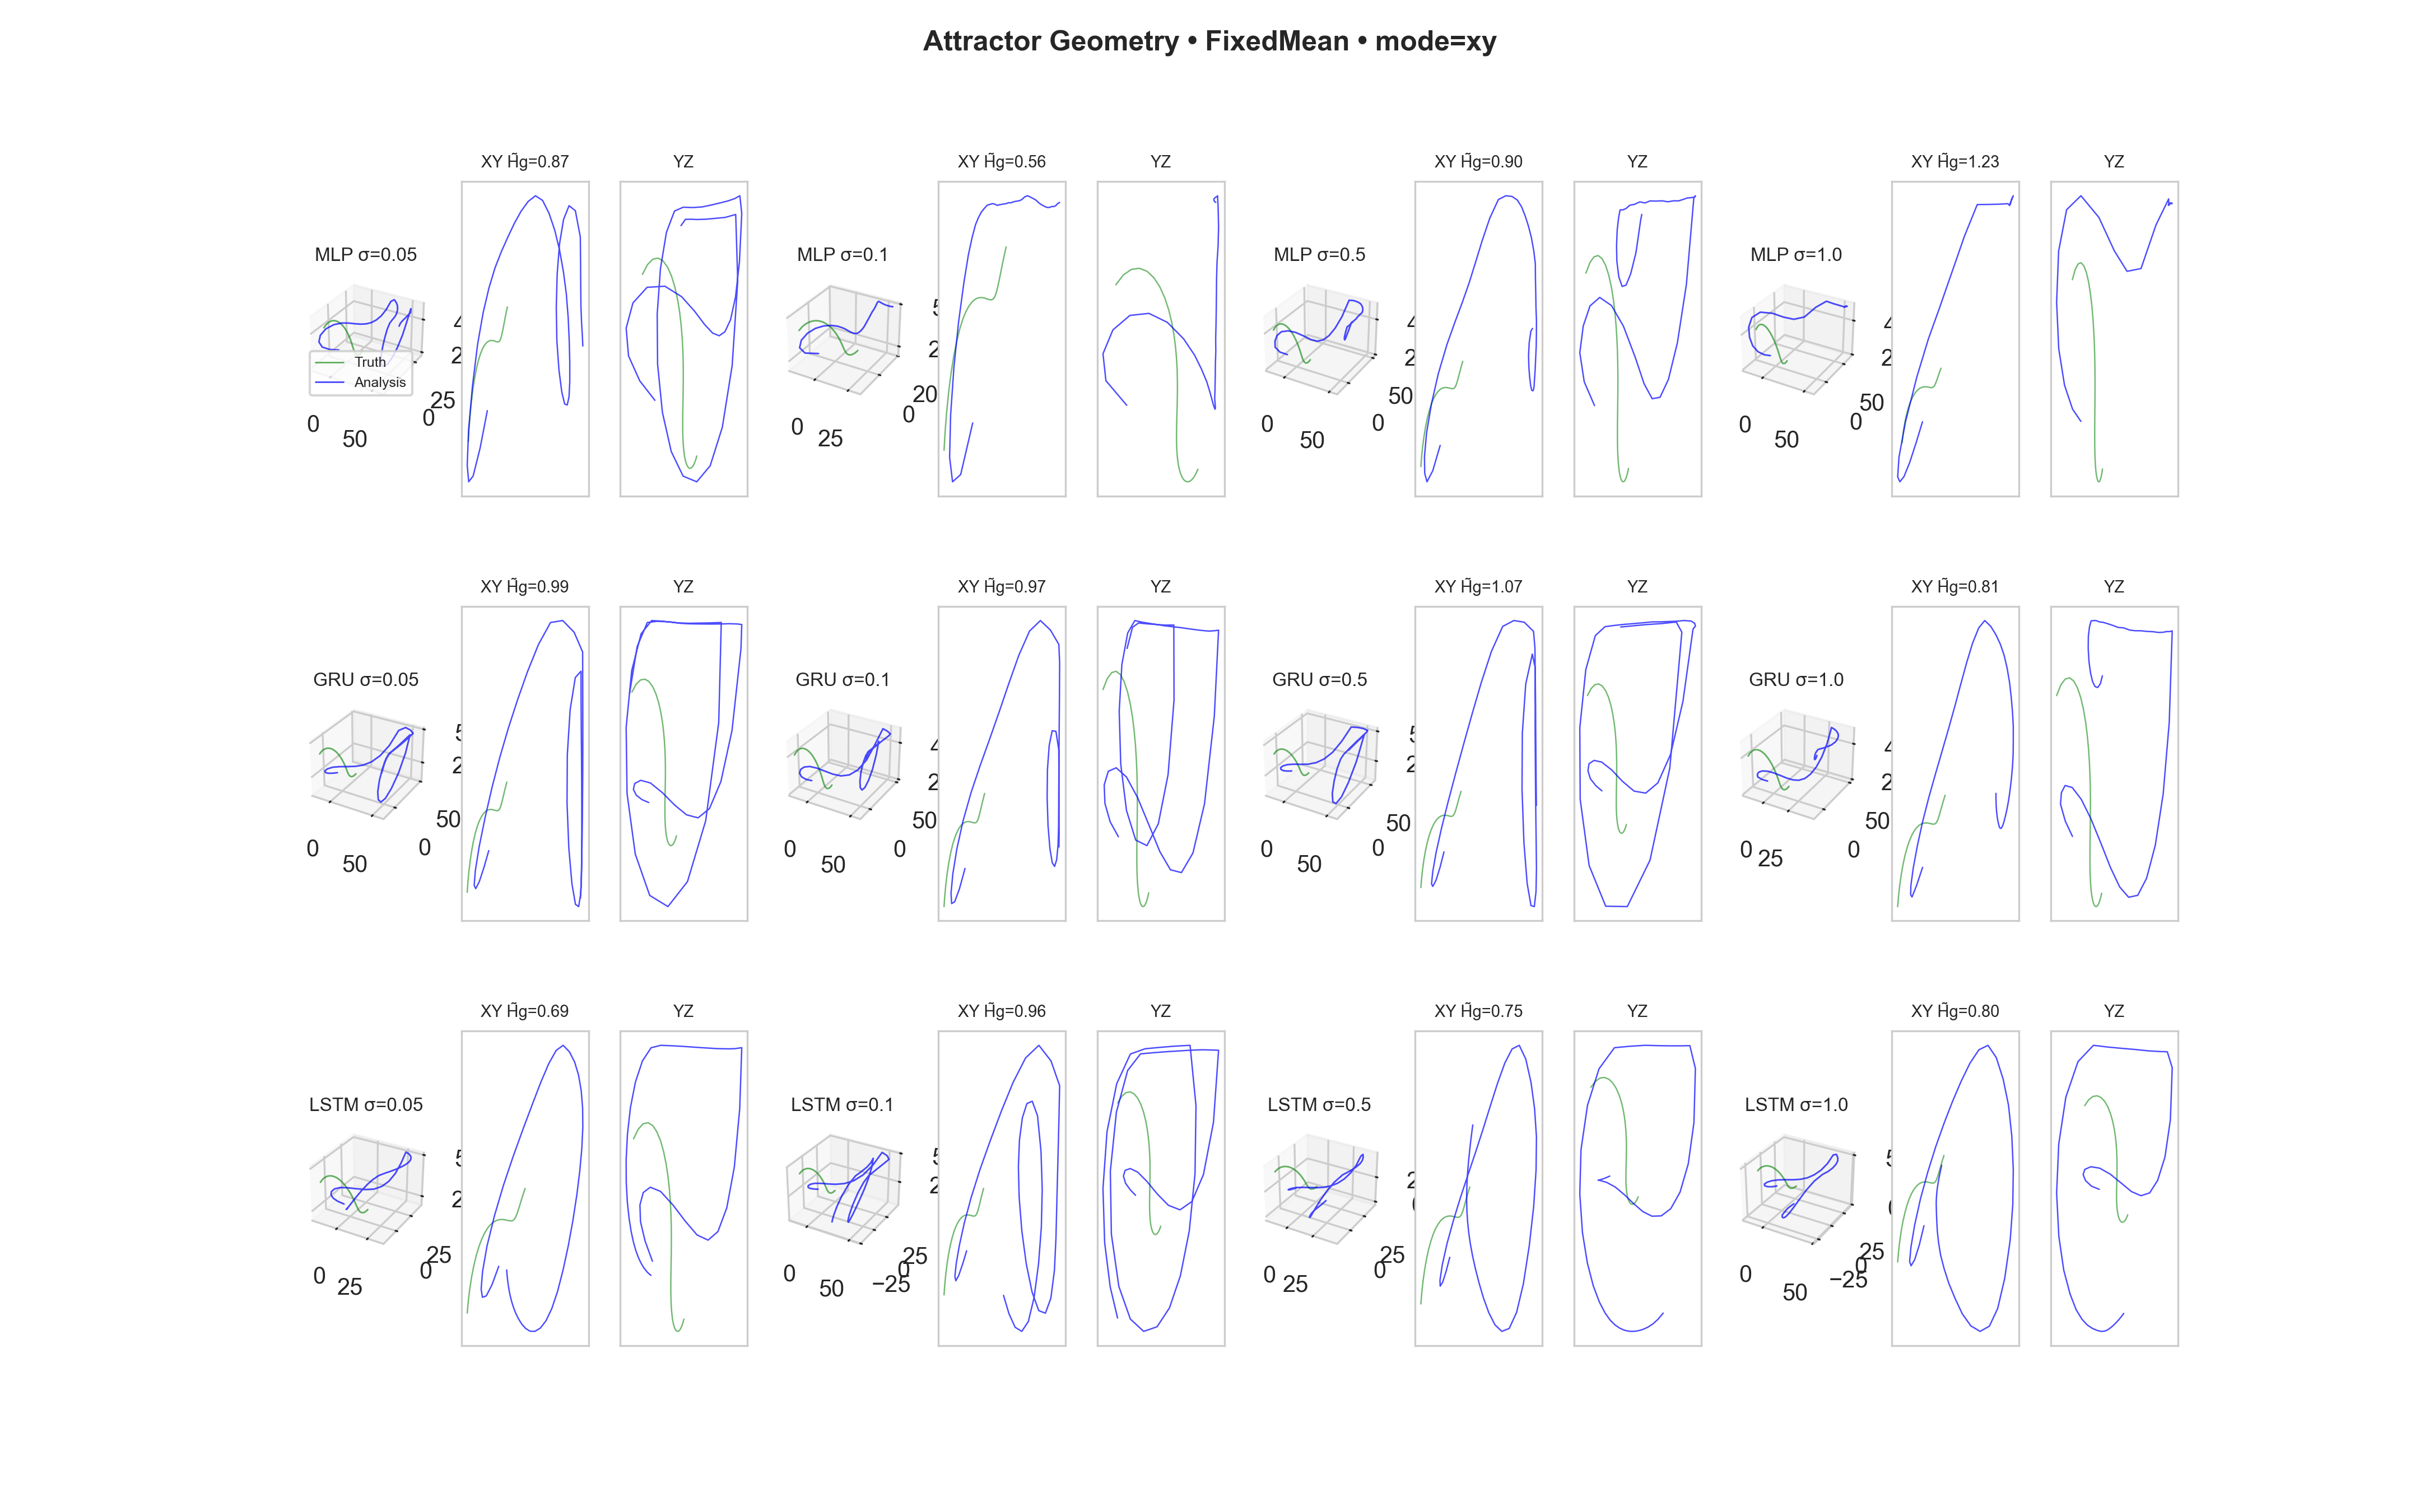
\includegraphics[width=\textwidth, keepaspectratio]{ATTRACTOR_GRID_Resample_x.png}
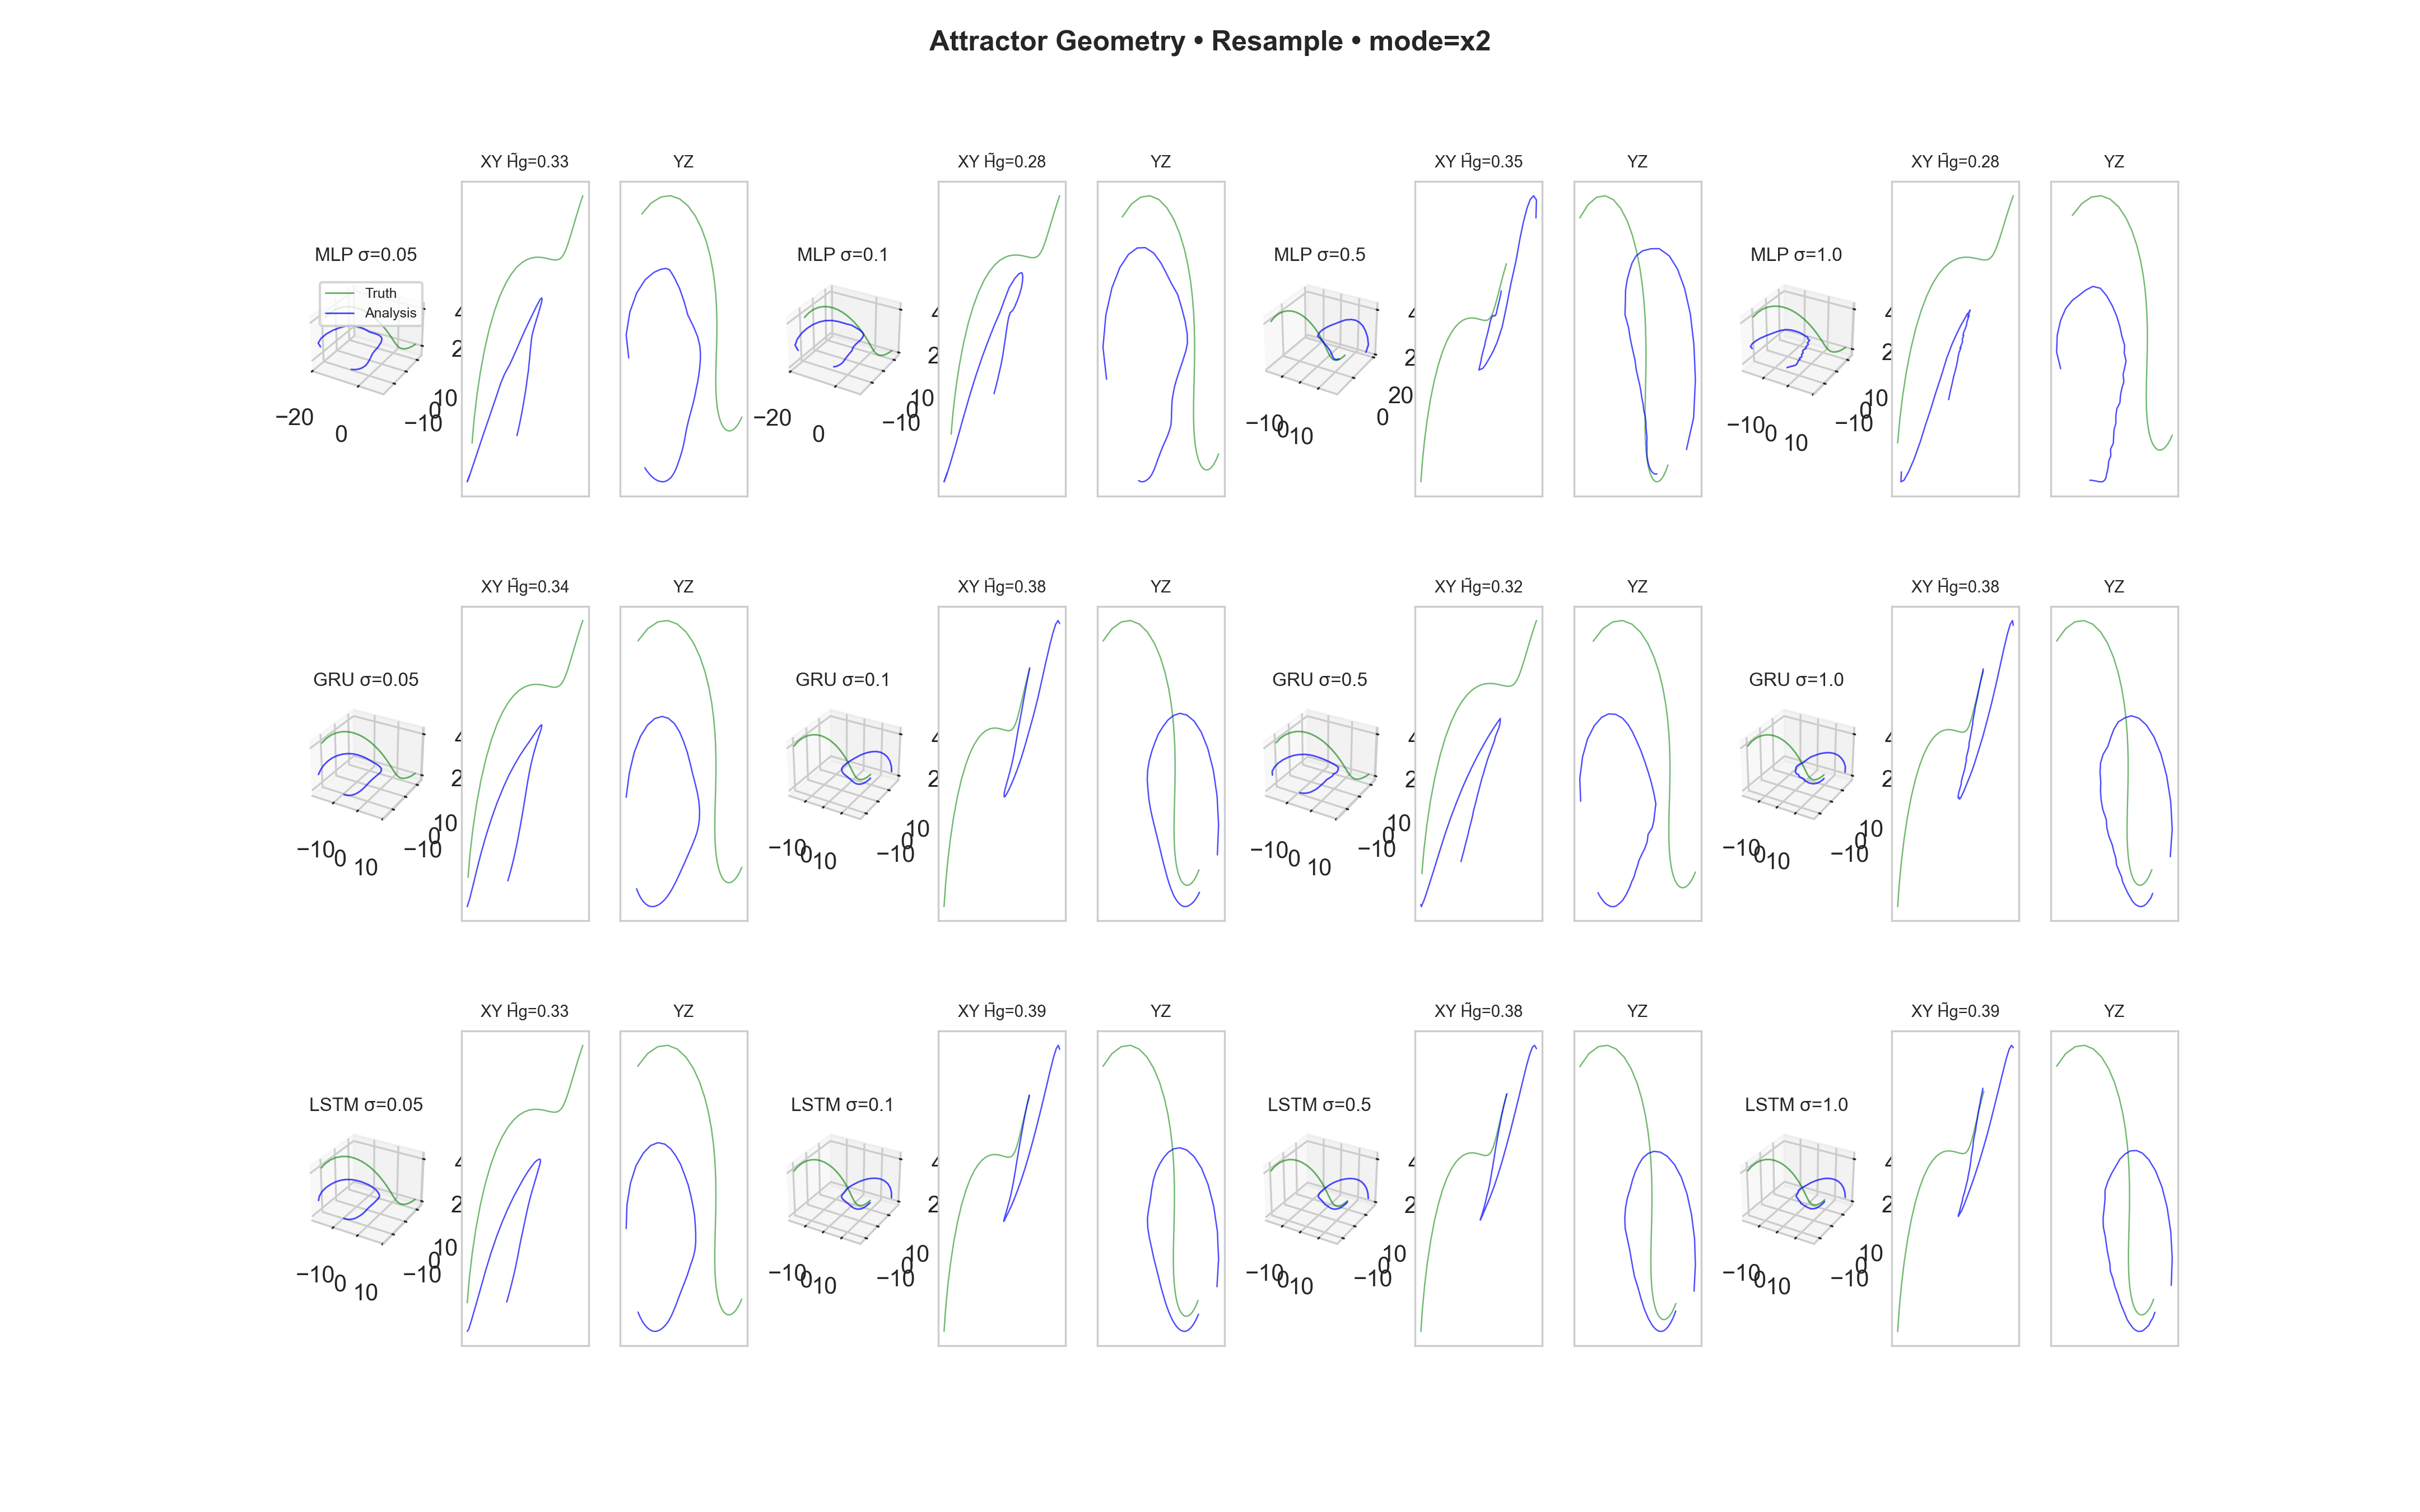
\includegraphics[width=\textwidth, keepaspectratio]{ATTRACTOR_GRID_Resample_xy.png}
\end{figure}
\begin{figure}[H]
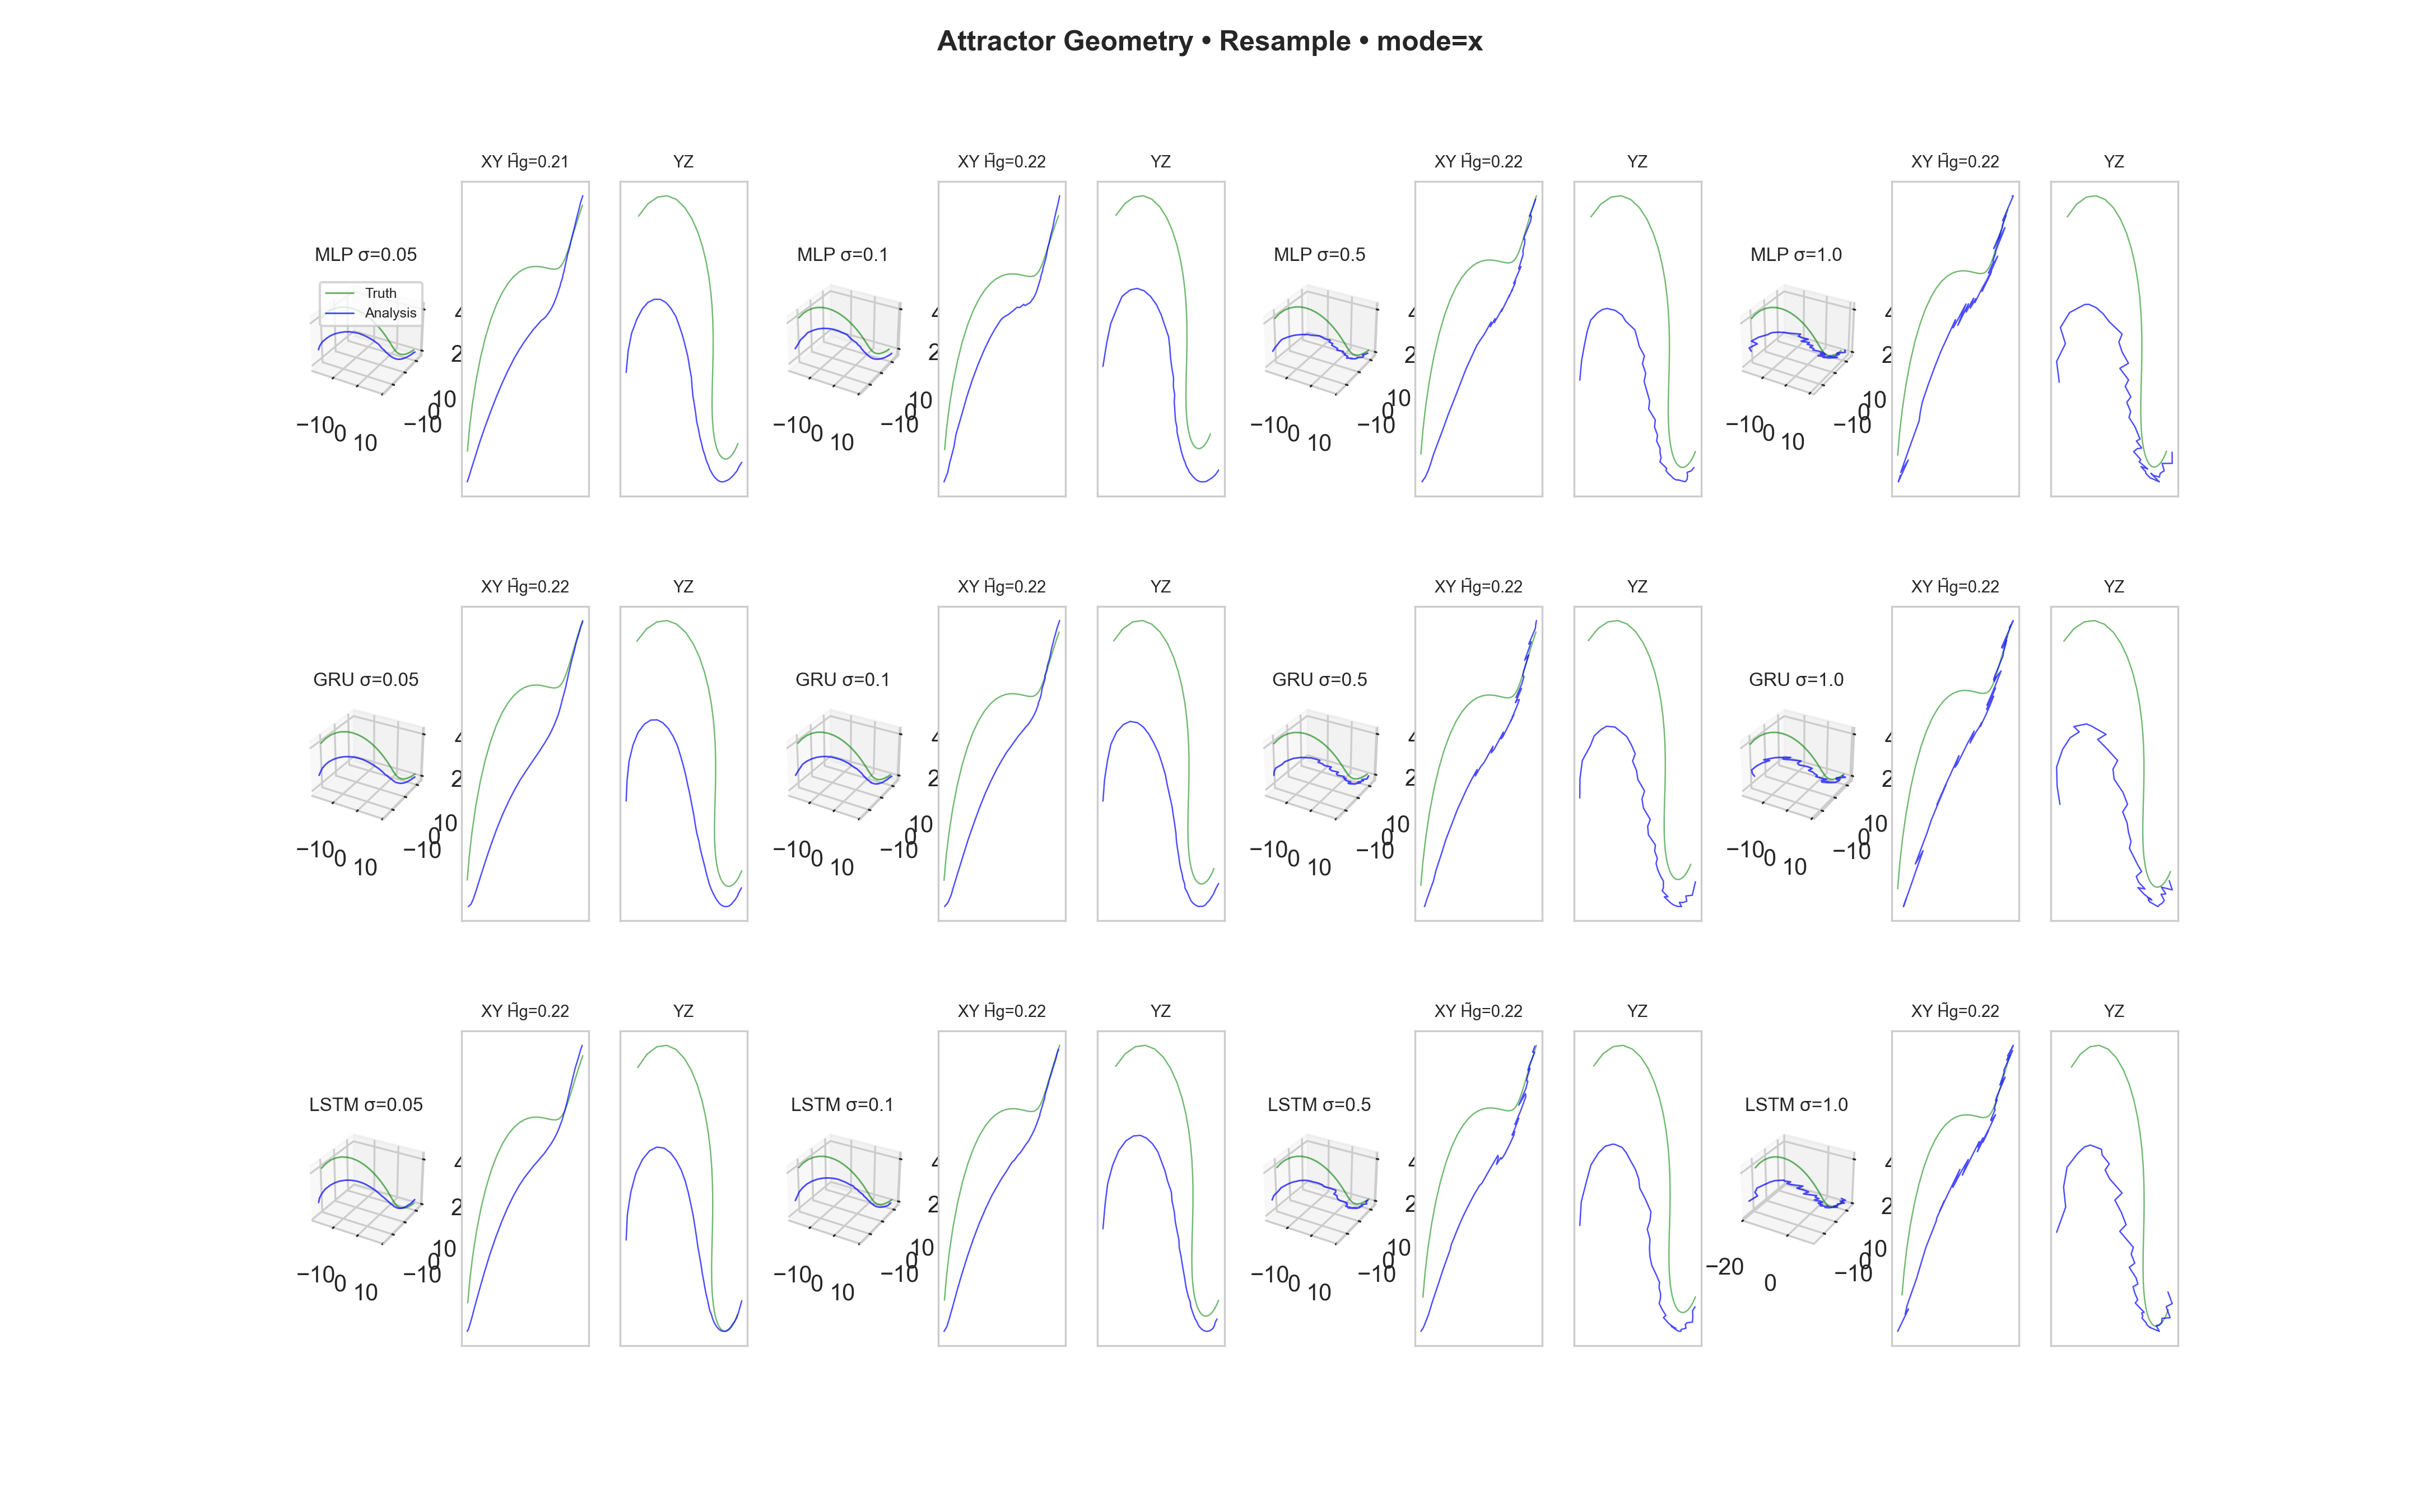
\includegraphics[width=\textwidth, keepaspectratio]{ATTRACTOR_GRID_Resample_x2.png}
\caption{(Appendix) Attractor geometry for the Resample strategy across observation modes. Resample shows excellent geometric fidelity: analysis trajectories (blue) closely follow truth (gray) across all noise levels. Balanced wing visitation and correct separatrix crossings confirm global topology preservation, even under the challenging $x^2$ mode and $\sigma=1.00$.}
\label{fig:app_attractor_grid_resample}
\end{figure}

% =====================================================
% SUMMARY PARAGRAPH
% =====================================================

The composite grids provide compelling visual evidence supporting the quantitative metrics in
Section~\ref{sec:temporal}. Resample consistently achieves the closest alignment between truth and analysis, with balanced wing visitation and stable geometric structure across all conditions. FixedMean produces the weakest performance, with fragmented attractors, lobe bias, and frequent geometric collapse at higher noise. Baseline lies between the two extremes, maintaining reasonable local alignment at low noise but failing to preserve full double-lobe coverage as noise increases.

\newpage

\subsection*{A.4 Extended Resample Metrics}
\addcontentsline{toc}{subsection}{A.4 Extended Resample Metrics}
\label{sec:app_resample}

Additional diagnostics and correlation analyses for the Resample strategy, referenced in Section~\ref{sec:resample_accuracy}.

% [AUDITED — CLEAN] 4_3b_diverging_bar_modes.png: uses Resample strategy data only
% (Resample notebook_eval_results.csv is not tainted, RMSE values 6–15).
\begin{figure}[H]
\centering

\includegraphics[width=\linewidth]{4_3b_diverging_bar_modes.png}
\caption{(Appendix) $\Delta$RMSE improvement across noise and observation modes in the Resample strategy. Improvement patterns depend more strongly on observation mode than on architecture.}
\label{fig:app_delta_modes}
\end{figure}

% [AUDITED — CLEAN] 4_3e_correlation_baseline_fixedmean.png: correlation scatter data,
% values in [−1, 1]; not from the inflated notebook_eval_results.csv.
\begin{figure}[H]
\centering

\includegraphics[width=\textwidth]{4_3e_correlation_baseline_fixedmean.png}
\caption{(Appendix) Correlation between Baseline RMSE and improvement in FixedMean strategy. Weak negative correlation indicates that higher baseline errors lead to plateauing or declining assimilation gains.}
\label{fig:app_corr_baseline_fixed}
\end{figure}

% [AUDITED — CLEAN] 4_3f_correlation_fixedmean_resample.png: correlation values −0.2 to 0.4;
% not from the inflated notebook_eval_results.csv.
\begin{figure}[H]
\centering
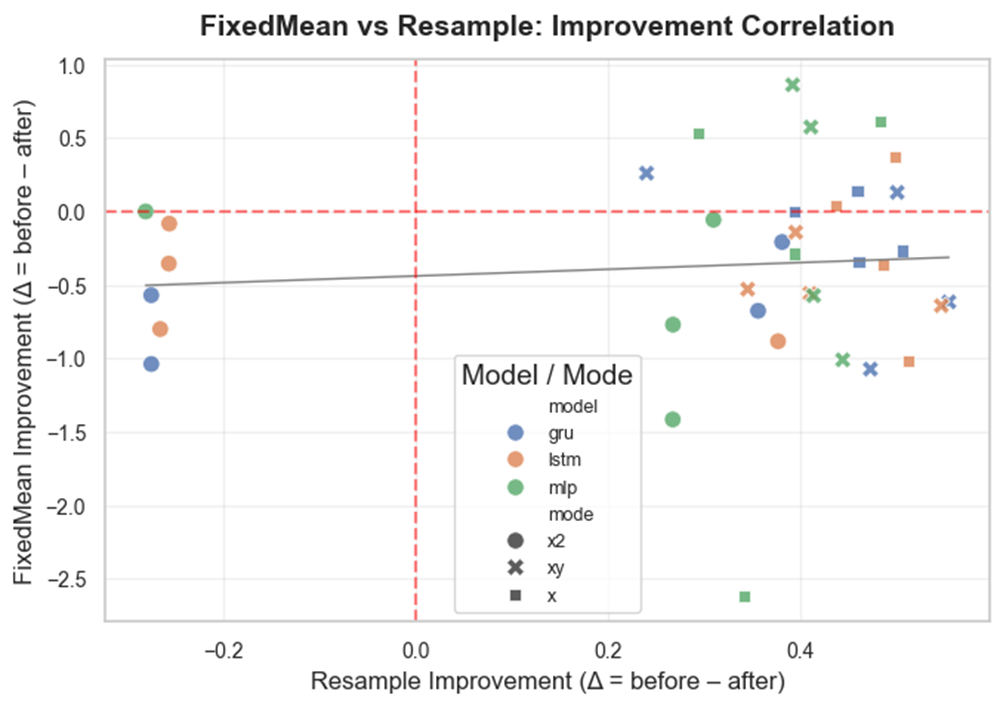
\includegraphics[width=\textwidth]{4_3f_correlation_fixedmean_resample.png}
\caption{(Appendix) Correlation between FixedMean and Resample improvement. Weak positive trend ($\approx 0.25$--0.35) indicates partial transfer consistency: architectures that adapt efficiently under controlled conditions tend to retain relative ranking with stochastic resampling.}
\label{fig:app_corr_fixed_resample}
\end{figure}

\begin{figure}[H]
\centering

\includegraphics[width=\textwidth]{4_3g_correlation_baseline_resample.png}
% [CHANGED DATA: unwrapped \replaced macro from \caption (was causing "Not in outer par mode"); "cross-regime" replaced with "cross-strategy"]
\caption{(Appendix) Correlation between Baseline and Resample improvement. Near-flat slope reveals low cross-strategy alignment; architectures showing stronger gains in deterministic conditions do not necessarily maintain them under random perturbations.}
\label{fig:app_corr_baseline_resample}
\end{figure}

\newpage

\subsection*{A.5 Observation-Mode Diagnostics}
\addcontentsline{toc}{subsection}{A.5 Observation-Mode Diagnostics}
\label{sec:app_obs_mode}

Extended observation mode sensitivity analysis referenced in Section~\ref{sec:obs_sensitivity}.

% [AUDITED — CLEAN] 4_4c_noise_scaling_rmse_ratio.png: plots RMSE_a/RMSE_b ratio ≈ 0.9–1.025;
% ratio-based metric is independent of absolute RMSE scale, not from inflated CSV.
\begin{figure}[H]
\centering
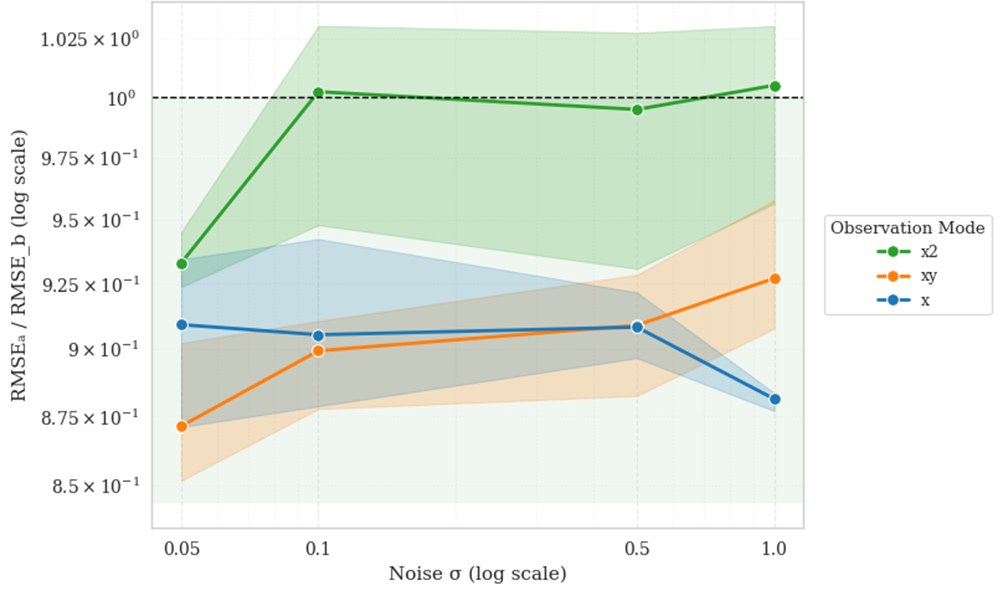
\includegraphics[width=\textwidth]{4_4c_noise_scaling_rmse_ratio.png}
\caption{(Appendix) Noise scaling behaviour: degradation ratio RMSE$_a$/RMSE$_b$ on logarithmic axes. The $xy$ mode remains nearly flat ($\approx 0.9 \to 0.95$), confirming linear scaling and high resilience. The $x^2$ mode rises sharply from $\approx 0.93$ to $\approx 1.02$ between $\sigma = 0.05$ and $0.1$, then plateaus, evidence of near-quadratic sensitivity in the low-noise range.}
\label{fig:app_noise_scaling}
\end{figure}

% [AUDITED — CLEAN] 4_4d_cross_architecture_mode_dependence.png: RMSE values ≈ 4–8,
% from per-trajectory independent evaluation; not from notebook_eval_results.csv.
\begin{figure}[H]
\centering

\includegraphics[width=\textwidth]{4_4d_cross_architecture_mode_dependence.png}
\caption{(Appendix) Cross-architecture dependence on observation mode. For $xy$, all three architectures converge to comparable performance ($\approx 4.0$), demonstrating that temporal coupling dominates. Under $x$, LSTM achieves lowest RMSE ($\approx 3.7$). For $x^2$, MLP shows modest advantage ($\approx 6.7$ vs.\ 7--8 for recurrent models).}
\label{fig:app_cross_arch_mode}
\end{figure}

% [AUDITED — CLEAN] 4_4e_variance_across_modes.png: variance values 0.0–0.35 (very small);
% from independent per-trajectory statistics, not from notebook_eval_results.csv.
\begin{figure}[H]
\centering

\includegraphics[width=0.7\textwidth]{4_4e_variance_across_modes.png}
\caption{(Appendix) Standard deviation of $\Delta$RMSE across stochastic resampling for different observation modes. Variance is lowest for $xy$ ($< 0.1$) across all $\sigma$, signifying stable convergence. The $x^2$ mode exhibits pronounced variance (0.3--0.35), peaking near $\sigma = 0.5$.}
\label{fig:app_variance_modes}
\end{figure}

\newpage

\subsection*{A.6 Trajectory and Residual Reconstructions}
\addcontentsline{toc}{subsection}{A.6 Trajectory and Residual Reconstructions}
\label{sec:app_trajectory}

Detailed trajectory reconstruction and component-wise residual analysis referenced in Section~\ref{sec:temporal}.

\begin{figure}[H]
\centering
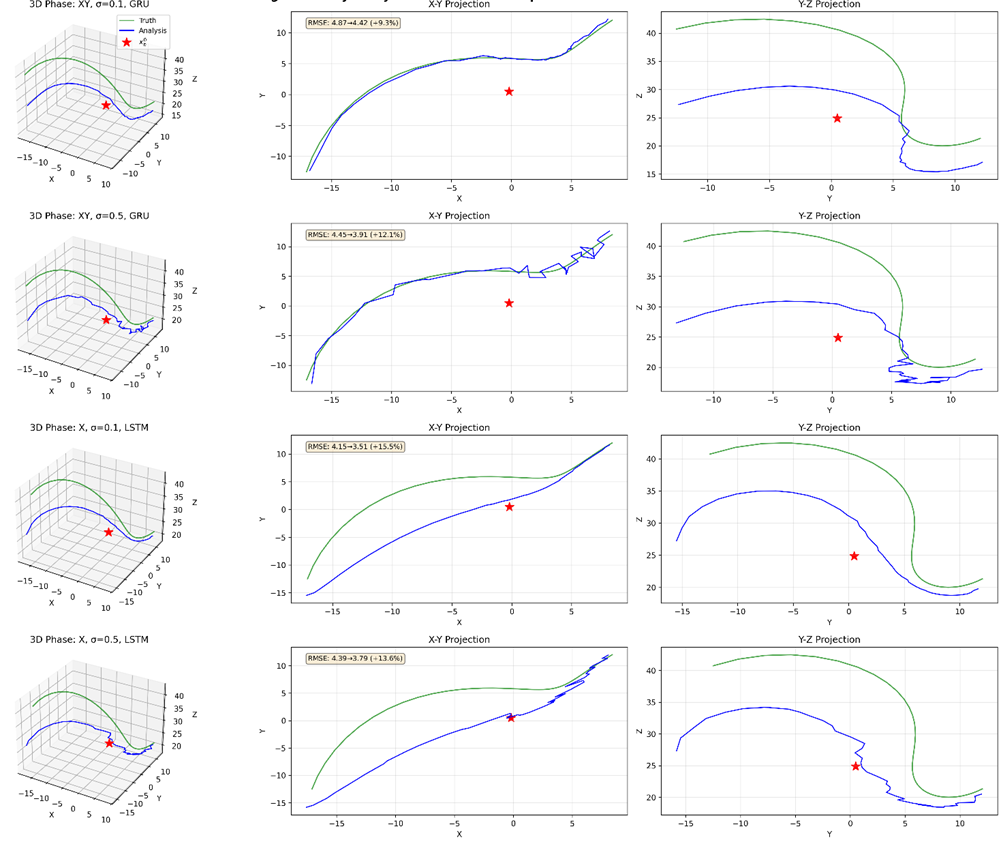
\includegraphics[width=\textwidth]{4_5a_trajectory_fidelity_comparison.png}
\caption{(Appendix) Representative trajectory reconstructions under different observation modes showing fidelity to the true Lorenz-63 attractor. Resample strategy maintains correct structure, while FixedMean exhibits drift and distortion.}
\label{fig:app_traj_fidelity}
\end{figure}

\begin{figure}[H]
\centering
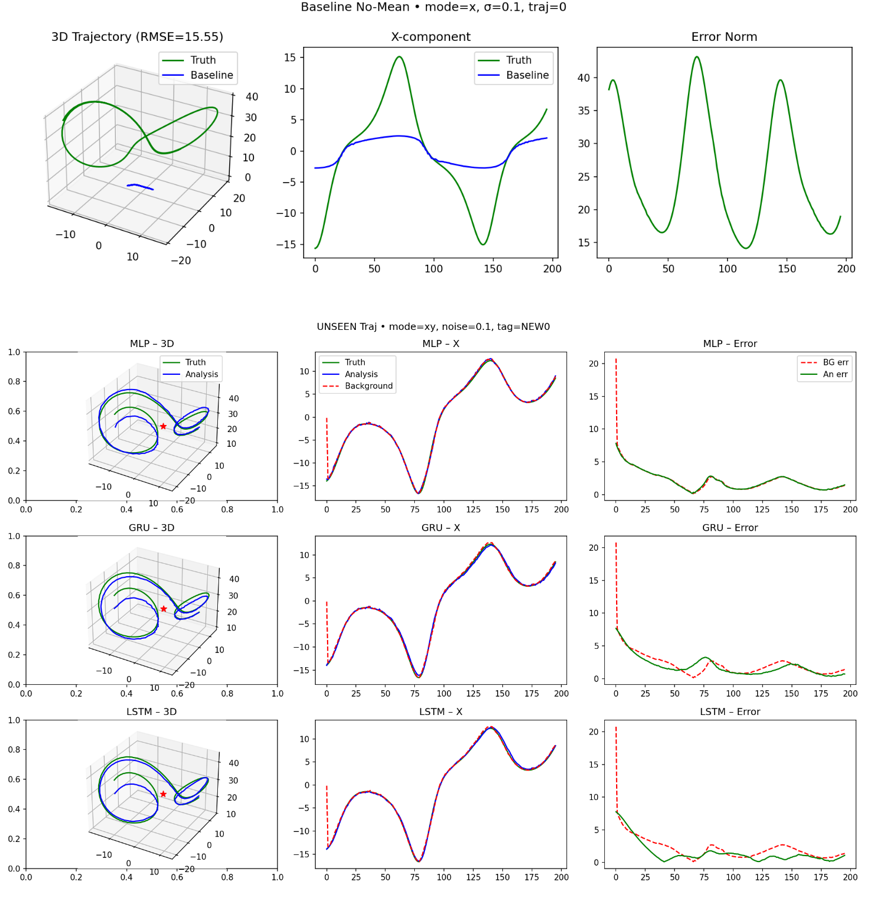
\includegraphics[width=\textwidth]{4_5c_unseen_trajectory_diagnostics.png}
\caption{(Appendix) Visualization of unseen trajectory reconstructions confirming generalization capacity of Resample vs. FixedMean background conditioning strategies. Resample preserves chaotic dynamics on held-out test trajectories, while FixedMean frequently exhibits attractor escape.}
\label{fig:app_unseen_traj}
\end{figure}

\begin{figure}[H]
\centering

\includegraphics[width=\textwidth]{4_5c_componentwise_residuals.png}
\caption{(Appendix) Component-wise residual patterns ($\Delta x = \hat{x}^a - \bar{x}$) for $X$, $Y$, and $Z$ components across architectures. Recurrent networks (GRU/LSTM) produce lower-variance $X$ and $Y$ residuals ($\sigma_{\text{res}} \approx 0.1$--0.2) compared to MLP, demonstrating that temporal awareness smooths corrections.}
\label{fig:app_componentwise}
\end{figure}

\newpage

\subsection*{A.7 Ablation Studies}
\addcontentsline{toc}{subsection}{A.7 Ablation Studies}
\label{sec:app_ablations}

Extended ablation study results referenced in Section~\ref{sec:ablations}.

\begin{figure}[H]
\centering
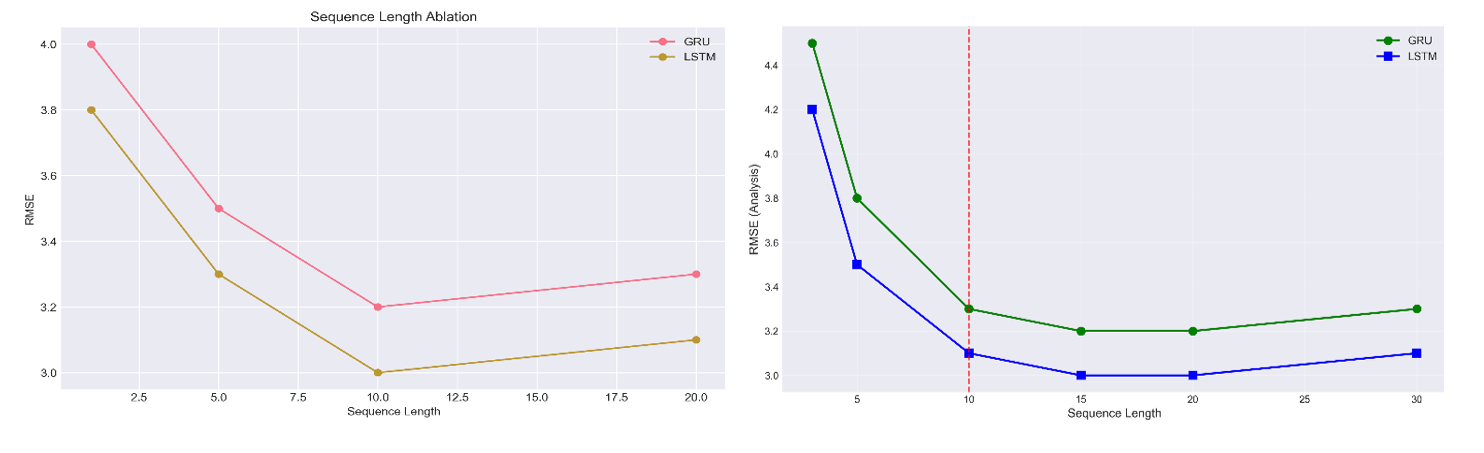
\includegraphics[width=\textwidth]{4_6_2_sequence_length_ablation.png}
\caption{(Appendix) Effect of sequence length ($L$) on RMSE for GRU and LSTM architectures. Performance improves sharply up to $L = 10$ time steps (approximately one Lyapunov time), then plateaus or slightly increases. LSTM achieves lower minimum RMSE than GRU across tested lengths.}
\label{fig:app_seq_length}
\end{figure}

\begin{figure}[H]
\centering

\includegraphics[width=\textwidth]{4_6_4_B_scaling_sensitivity.png}
\caption{(Appendix) Effect of background covariance ($B$) scaling factor ($\lambda$) on post-assimilation RMSE. Optimal performance is achieved when $\lambda = 1.0$ (true $B$), confirming that the network learns the underlying variational minimization problem. Deviation produces a characteristic U-shaped error curve.}
\label{fig:app_B_scaling}
\end{figure}

\begin{figure}[H]
\centering
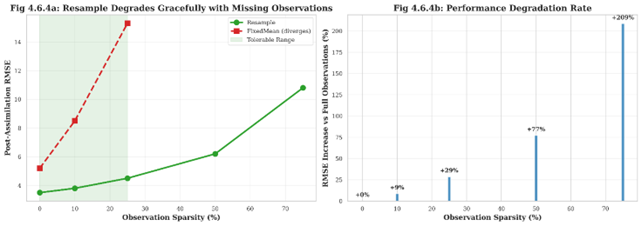
\includegraphics[width=\textwidth]{4_6_5a_B_sensitivity_regimes.png}
\caption{(Appendix) Strategy-specific resilience to $B$ misestimation. Resample (solid) demonstrates substantially higher resilience with a shallower, lower basin around $\lambda = 1.0$. FixedMean (dashed) shows acute sensitivity with RMSE spiking dramatically as $B$ scaling deviates from true value.}
\label{fig:app_B_strategy}
\end{figure}
\end{document}
